% Options for packages loaded elsewhere
% Options for packages loaded elsewhere
\PassOptionsToPackage{unicode}{hyperref}
\PassOptionsToPackage{hyphens}{url}
\PassOptionsToPackage{dvipsnames,svgnames,x11names}{xcolor}
%
\documentclass[
  letterpaper,
  DIV=11,
  numbers=noendperiod]{scrreprt}
\usepackage{xcolor}
\usepackage{amsmath,amssymb}
\setcounter{secnumdepth}{2}
\usepackage{iftex}
\ifPDFTeX
  \usepackage[T1]{fontenc}
  \usepackage[utf8]{inputenc}
  \usepackage{textcomp} % provide euro and other symbols
\else % if luatex or xetex
  \usepackage{unicode-math} % this also loads fontspec
  \defaultfontfeatures{Scale=MatchLowercase}
  \defaultfontfeatures[\rmfamily]{Ligatures=TeX,Scale=1}
\fi
\usepackage{lmodern}
\ifPDFTeX\else
  % xetex/luatex font selection
\fi
% Use upquote if available, for straight quotes in verbatim environments
\IfFileExists{upquote.sty}{\usepackage{upquote}}{}
\IfFileExists{microtype.sty}{% use microtype if available
  \usepackage[]{microtype}
  \UseMicrotypeSet[protrusion]{basicmath} % disable protrusion for tt fonts
}{}
\makeatletter
\@ifundefined{KOMAClassName}{% if non-KOMA class
  \IfFileExists{parskip.sty}{%
    \usepackage{parskip}
  }{% else
    \setlength{\parindent}{0pt}
    \setlength{\parskip}{6pt plus 2pt minus 1pt}}
}{% if KOMA class
  \KOMAoptions{parskip=half}}
\makeatother
% Make \paragraph and \subparagraph free-standing
\makeatletter
\ifx\paragraph\undefined\else
  \let\oldparagraph\paragraph
  \renewcommand{\paragraph}{
    \@ifstar
      \xxxParagraphStar
      \xxxParagraphNoStar
  }
  \newcommand{\xxxParagraphStar}[1]{\oldparagraph*{#1}\mbox{}}
  \newcommand{\xxxParagraphNoStar}[1]{\oldparagraph{#1}\mbox{}}
\fi
\ifx\subparagraph\undefined\else
  \let\oldsubparagraph\subparagraph
  \renewcommand{\subparagraph}{
    \@ifstar
      \xxxSubParagraphStar
      \xxxSubParagraphNoStar
  }
  \newcommand{\xxxSubParagraphStar}[1]{\oldsubparagraph*{#1}\mbox{}}
  \newcommand{\xxxSubParagraphNoStar}[1]{\oldsubparagraph{#1}\mbox{}}
\fi
\makeatother


\usepackage{longtable,booktabs,array}
\usepackage{calc} % for calculating minipage widths
% Correct order of tables after \paragraph or \subparagraph
\usepackage{etoolbox}
\makeatletter
\patchcmd\longtable{\par}{\if@noskipsec\mbox{}\fi\par}{}{}
\makeatother
% Allow footnotes in longtable head/foot
\IfFileExists{footnotehyper.sty}{\usepackage{footnotehyper}}{\usepackage{footnote}}
\makesavenoteenv{longtable}
\usepackage{graphicx}
\makeatletter
\newsavebox\pandoc@box
\newcommand*\pandocbounded[1]{% scales image to fit in text height/width
  \sbox\pandoc@box{#1}%
  \Gscale@div\@tempa{\textheight}{\dimexpr\ht\pandoc@box+\dp\pandoc@box\relax}%
  \Gscale@div\@tempb{\linewidth}{\wd\pandoc@box}%
  \ifdim\@tempb\p@<\@tempa\p@\let\@tempa\@tempb\fi% select the smaller of both
  \ifdim\@tempa\p@<\p@\scalebox{\@tempa}{\usebox\pandoc@box}%
  \else\usebox{\pandoc@box}%
  \fi%
}
% Set default figure placement to htbp
\def\fps@figure{htbp}
\makeatother


% definitions for citeproc citations
\NewDocumentCommand\citeproctext{}{}
\NewDocumentCommand\citeproc{mm}{%
  \begingroup\def\citeproctext{#2}\cite{#1}\endgroup}
\makeatletter
 % allow citations to break across lines
 \let\@cite@ofmt\@firstofone
 % avoid brackets around text for \cite:
 \def\@biblabel#1{}
 \def\@cite#1#2{{#1\if@tempswa , #2\fi}}
\makeatother
\newlength{\cslhangindent}
\setlength{\cslhangindent}{1.5em}
\newlength{\csllabelwidth}
\setlength{\csllabelwidth}{3em}
\newenvironment{CSLReferences}[2] % #1 hanging-indent, #2 entry-spacing
 {\begin{list}{}{%
  \setlength{\itemindent}{0pt}
  \setlength{\leftmargin}{0pt}
  \setlength{\parsep}{0pt}
  % turn on hanging indent if param 1 is 1
  \ifodd #1
   \setlength{\leftmargin}{\cslhangindent}
   \setlength{\itemindent}{-1\cslhangindent}
  \fi
  % set entry spacing
  \setlength{\itemsep}{#2\baselineskip}}}
 {\end{list}}
\usepackage{calc}
\newcommand{\CSLBlock}[1]{\hfill\break\parbox[t]{\linewidth}{\strut\ignorespaces#1\strut}}
\newcommand{\CSLLeftMargin}[1]{\parbox[t]{\csllabelwidth}{\strut#1\strut}}
\newcommand{\CSLRightInline}[1]{\parbox[t]{\linewidth - \csllabelwidth}{\strut#1\strut}}
\newcommand{\CSLIndent}[1]{\hspace{\cslhangindent}#1}



\setlength{\emergencystretch}{3em} % prevent overfull lines

\providecommand{\tightlist}{%
  \setlength{\itemsep}{0pt}\setlength{\parskip}{0pt}}



 


\usepackage{fvextra}
\DefineVerbatimEnvironment{Highlighting}{Verbatim}{
  breaklines,
  breakanywhere=true,
  breakautoindent=true,
  breaksymbol=\textcolor{gray}{\tiny\ensuremath{\hookrightarrow}},
  commandchars=\\\{\}
}


\usepackage{float}
\floatplacement{fig}{!hp}
\floatplacement{table}{!hp}

\usepackage{caption}
\captionsetup{justification=raggedright, singlelinecheck=false}
\KOMAoption{captions}{tableheading,figureheading}
\makeatletter
\@ifpackageloaded{float}{}{\usepackage{float}}
\floatstyle{plain}
\@ifundefined{c@chapter}{\newfloat{suppfig}{h}{losuppfig}}{\newfloat{suppfig}{h}{losuppfig}[chapter]}
\floatname{suppfig}{Figure S}
\floatstyle{plaintop}
\restylefloat{suppfig}
\newcommand*\quartosuppfigref[1]{Figure \hyperref[#1]{S\ref{#1}}}
\@ifpackageloaded{caption}{}{\usepackage{caption}}
\DeclareCaptionLabelFormat{quartosuppfigreflabelformat}{#1#2}
\captionsetup[suppfig]{labelformat=quartosuppfigreflabelformat}
\newcommand*\listofsuppfigs{\listof{suppfig}{List of Supplementary Figures}}
\makeatother
\makeatletter
\@ifpackageloaded{float}{}{\usepackage{float}}
\floatstyle{plain}
\@ifundefined{c@chapter}{\newfloat{supptbl}{h}{losupptbl}}{\newfloat{supptbl}{h}{losupptbl}[chapter]}
\floatname{supptbl}{Table S}
\floatstyle{plaintop}
\restylefloat{supptbl}
\newcommand*\quartosupptblref[1]{Table \hyperref[#1]{S\ref{#1}}}
\@ifpackageloaded{caption}{}{\usepackage{caption}}
\DeclareCaptionLabelFormat{quartosupptblreflabelformat}{#1#2}
\captionsetup[supptbl]{labelformat=quartosupptblreflabelformat}
\newcommand*\listofsupptbls{\listof{supptbl}{List of Supplementary Tables}}
\makeatother
\makeatletter
\@ifpackageloaded{tcolorbox}{}{\usepackage[skins,breakable]{tcolorbox}}
\@ifpackageloaded{fontawesome5}{}{\usepackage{fontawesome5}}
\definecolor{quarto-callout-color}{HTML}{909090}
\definecolor{quarto-callout-note-color}{HTML}{0758E5}
\definecolor{quarto-callout-important-color}{HTML}{CC1914}
\definecolor{quarto-callout-warning-color}{HTML}{EB9113}
\definecolor{quarto-callout-tip-color}{HTML}{00A047}
\definecolor{quarto-callout-caution-color}{HTML}{FC5300}
\definecolor{quarto-callout-color-frame}{HTML}{acacac}
\definecolor{quarto-callout-note-color-frame}{HTML}{4582ec}
\definecolor{quarto-callout-important-color-frame}{HTML}{d9534f}
\definecolor{quarto-callout-warning-color-frame}{HTML}{f0ad4e}
\definecolor{quarto-callout-tip-color-frame}{HTML}{02b875}
\definecolor{quarto-callout-caution-color-frame}{HTML}{fd7e14}
\makeatother
\makeatletter
\@ifpackageloaded{bookmark}{}{\usepackage{bookmark}}
\makeatother
\makeatletter
\@ifpackageloaded{caption}{}{\usepackage{caption}}
\AtBeginDocument{%
\ifdefined\contentsname
  \renewcommand*\contentsname{Table of contents}
\else
  \newcommand\contentsname{Table of contents}
\fi
\ifdefined\listfigurename
  \renewcommand*\listfigurename{List of Figures}
\else
  \newcommand\listfigurename{List of Figures}
\fi
\ifdefined\listtablename
  \renewcommand*\listtablename{List of Tables}
\else
  \newcommand\listtablename{List of Tables}
\fi
\ifdefined\figurename
  \renewcommand*\figurename{Supplementary Figure}
\else
  \newcommand\figurename{Supplementary Figure}
\fi
\ifdefined\tablename
  \renewcommand*\tablename{Supplementary Table}
\else
  \newcommand\tablename{Supplementary Table}
\fi
}
\@ifpackageloaded{float}{}{\usepackage{float}}
\floatstyle{ruled}
\@ifundefined{c@chapter}{\newfloat{codelisting}{h}{lop}}{\newfloat{codelisting}{h}{lop}[chapter]}
\floatname{codelisting}{Listing}
\newcommand*\listoflistings{\listof{codelisting}{List of Listings}}
\makeatother
\makeatletter
\makeatother
\makeatletter
\@ifpackageloaded{caption}{}{\usepackage{caption}}
\@ifpackageloaded{subcaption}{}{\usepackage{subcaption}}
\makeatother
\usepackage{bookmark}
\IfFileExists{xurl.sty}{\usepackage{xurl}}{} % add URL line breaks if available
\urlstyle{same}
\hypersetup{
  pdftitle={The Impact of Brief Mindfulness Training on Judgments of Confidence, Anxiety, and Difficulty While Answering Physics Questions},
  pdfauthor={Avital Pelakh; Eric Kuo; Melanie Good; Michael Tumminia; Sara Jahanian; Brian Galla; Timothy Nokes-Malach},
  colorlinks=true,
  linkcolor={blue},
  filecolor={Maroon},
  citecolor={Blue},
  urlcolor={Blue},
  pdfcreator={LaTeX via pandoc}}


\title{The Impact of Brief Mindfulness Training on Judgments of
Confidence, Anxiety, and Difficulty While Answering Physics Questions}
\usepackage{etoolbox}
\makeatletter
\providecommand{\subtitle}[1]{% add subtitle to \maketitle
  \apptocmd{\@title}{\par {\large #1 \par}}{}{}
}
\makeatother
\subtitle{Supplementary Materials}
\author{Avital Pelakh \and Eric Kuo \and Melanie Good \and Michael
Tumminia \and Sara Jahanian \and Brian Galla \and Timothy Nokes-Malach}
\date{2025-10-20}
\begin{document}
\maketitle
\begin{abstract}
We tested the impact of a mindfulness training intervention to improve
introductory physics students' experiences while answering physics
questions. We expected the intervention to reduce physics threat and to
increase students' confidence while reducing anxiety and judgments of
difficulty. We also tested whether domain-level physics threat mediated
the effects of the intervention on task judgments and whether the
effects differed by gender. To test these hypotheses one hundred and
forty-nine undergraduates were randomly assigned to receive either a
5-day mindfulness training intervention or no training (control). Both
groups answered physics questions before and directly after the
intervention and rated their confidence, anxiety, and difficulty for
each question. Mindfulness training led a greater increase in confidence
and a reduction in anxiety among women and non-binary students, but not
for men. The intervention also led to a reduction in judgments of
difficulty for all students. The association between mindfulness
training and self-reported anxiety among women and non-binary students
was mediated by reductions in physics threat (measured mid-week using
experience sampling). However, physics threat did not mediate any of the
other mindfulness training outcomes for confidence or difficulty. The
results are discussed in relation to a model of challenge and threat and
mindfulness applications.
\end{abstract}

\renewcommand*\contentsname{Table of contents}
{
\hypersetup{linkcolor=}
\setcounter{tocdepth}{2}
\tableofcontents
}

\bookmarksetup{startatroot}

\chapter*{Preface}\label{preface}
\addcontentsline{toc}{chapter}{Preface}

\markboth{Preface}{Preface}

\section*{Format Notes}\label{format-notes}
\addcontentsline{toc}{section}{Format Notes}

\markright{Format Notes}

Due to formatting constraints, some portions of the web-based materials
are not available in the PDF version (i.e., R code). Additionally,
tables and images may appear out of order. We've done our best to
provide reference links and documentation when this occurs. However, for
the best experience, please refer to the
\href{https://apelakh.github.io/pelakh-et-al-2025-supplement/}{web-based
version} of this Quarto book.

\section*{OSF Links}\label{osf-links}
\addcontentsline{toc}{section}{OSF Links}

\markright{OSF Links}

\begin{itemize}
\tightlist
\item
  \href{https://doi.org/10.17605/OSF.IO/WV6XT}{Project Home}
\item
  \href{https://doi.org/10.17605/OSF.IO/7RXVC}{Project Overview}
\item
  \href{https://doi.org/10.17605/OSF.IO/SA9W2}{Preregistration Plan}
\item
  \href{https://osf.io/fm8qx/}{Physics Task Materials}
\item
  \href{https://doi.org/10.31234/osf.io/sqpd5_v1}{Manuscript Preprint
  (PsyArXiv)}
\end{itemize}

\part{Supplementary Descriptive Text}

\chapter{Changes From the
Preregistration}\label{changes-from-the-preregistration}

All changes below are in reference to \textbf{Preregistration 3 --
Physics Task Outcomes} (\url{https://doi.org/10.17605/OSF.IO/SA9W2}).

\section{Wording Adjustments}\label{wording-adjustments}

The preregistration refers to the physics tasks as ``problem solving.''
We replaced this term with the phrase, ``answering physics questions.''
While all of our tasks assessed processes involved in problem solving
(i.e., problem categorization and conceptual understanding), the term
``problem solving'' is more commonly used among physics teachers in
reference to straightforward quantitative problems. Therefore, we
decided that ``answering physics questions'' was a more accurate
description of our tasks.

\section{Model Specifications}\label{model-specifications}

For RQ1, Hypotheses 1-3 in the main text: Instead of predicting outcomes
at posttest while controlling for baseline (Hypotheses 4-6 in the
preregistration), we used mixed-effects models that included
\emph{Timepoint} as a fixed effect, with baseline coded as 0 and
posttest coded as 1. This allowed us to effectively test multiple
hypotheses with fewer statistical models: baseline differences outlined
in Preregistration, Aim 1, and effects of mindfulness training outlined
in Preregistration, Aim 2. The advantage of this is that we were able to
simultaneously reduce the likelihood of committing type 1 error (by
running fewer individual tests) and lessen the burden on the reader.
Both methods produced the same pattern of results (see Model 1 for each
judgment type in Section~\ref{sec-preregistered} for results using
linear models as described in the preregistration).

\section{Gender Moderation}\label{gender-moderation}

While we expected gender to be an important covariate, we did not
preregister it as a moderator. Therefore, it is explicitly presented as
exploratory in the main text. Results of the mixed-effects models
without gender included as a moderator can be found here in
Supplementary Table~\ref{tbl-confidence-models}, Supplementary
Table~\ref{tbl-anxiety-models}, and Supplementary
Table~\ref{tbl-difficulty-models}. Results of the mediation analyses
without gender moderation can be found in
Section~\ref{sec-preregistered}. In both cases, the general pattern of
results is the same. Including gender as a moderator helped bring our
results into greater focus. For example, it revealed that overall
effects of the intervention on judgments of confidence and anxiety were
driven by women and non-binary students, while effects for judgements of
difficulty were stable across genders.

\section{Additional Control
Variables}\label{additional-control-variables}

We added several additional control variables to the models that were
not included in the preregistration. First, unlike what is specified in
the preregistration, we included baseline psychological threat as a
predictor in all the models, whereas it is only included in Aim 1: H1-H2
in the preregistration (testing baseline associations). Because our
final models simultaneously tested the hypotheses in Aim 1 (baseline
associations) and Aim 2 (effects of mindfulness on outcomes at
posttest), we included it to control for overall effects of
pre-intervention levels of psychological threat. We also included
item-level accuracy as a covariate in the models to rule out potential
confounding effects on perceptions. Including these variables had no
meaningful impact on the results, as shown in Supplementary
Table~\ref{tbl-confidence-models}, Supplementary
Table~\ref{tbl-anxiety-models}, and Supplementary
Table~\ref{tbl-difficulty-models}.

\section{Accuracy and Learning
Outcomes}\label{accuracy-and-learning-outcomes}

Finally, the analyses of accuracy performance and preparation for future
learning outcomes described in the preregistration are not included in
the main text. We did not find any effects of mindfulness training on
these outcomes (preregistered hypotheses 1, 4, and 5) or any mediation
effects (preregistered hypotheses 7 and 8). Therefore, we chose to
remove the details of these analyses from the main text to narrow the
scope of the paper. Those results are reported in these materials in
Supplementary Table~\ref{tbl-accuracy-results} and Supplementary
Table~\ref{tbl-pfl-results}.

\chapter{Examples of Physics Task
Items}\label{examples-of-physics-task-items}

\section{Physics Tasks, Part 1: Quantitative Problem
Solving}\label{physics-tasks-part-1-quantitative-problem-solving}

Students were provided with a general equation sheet for reference and
asked to solve a single quantitative problem. They were instructed to
use a blank sheet of paper to write out their work and final answer. The
quantitative problems were developed for this study by Drs. Melanie Good
and Eric Kuo (See Supplementary Figure~\ref{fig-quant}).

\begin{figure}[!hp]

\caption{\label{fig-quant}Sample Quantitative Physics Task Item}

\centering{

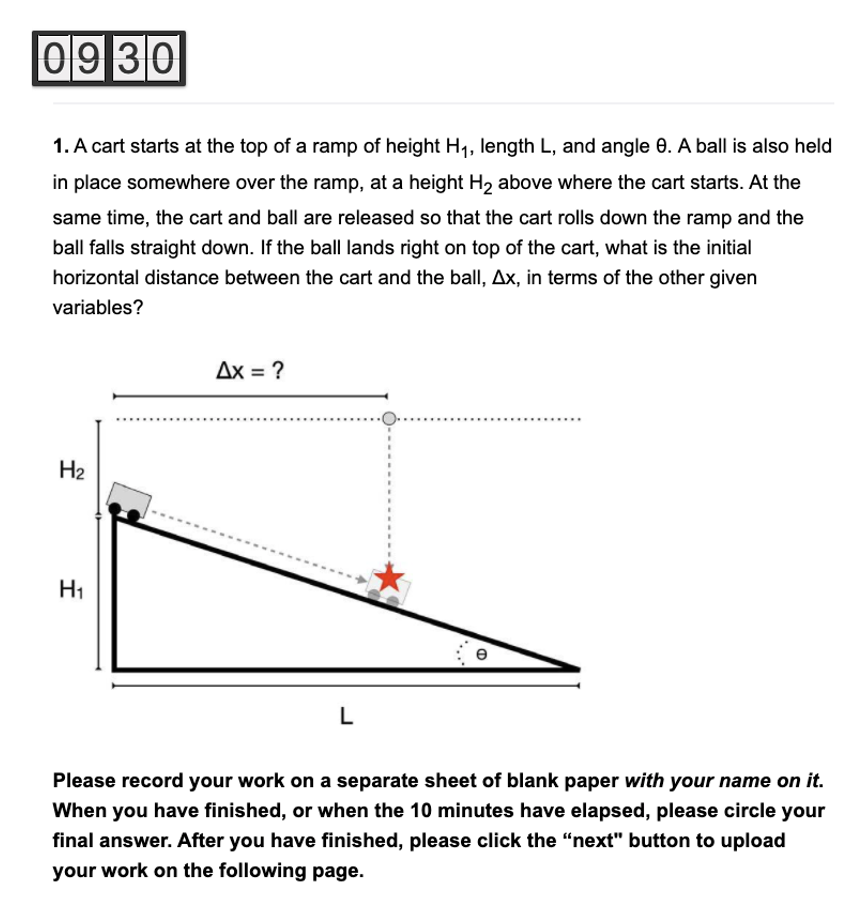
\includegraphics[width=0.75\linewidth,height=\textheight,keepaspectratio]{chapters/../img/sample-item-1.png}

}

\end{figure}%

\section{Physics Tasks, Part 2: Problem
Categorization}\label{physics-tasks-part-2-problem-categorization}

This part consisted of five items adapted from, and similar to, those
used in Hardiman, Dufresne, and Mestre (1989). For each item, a model
problem was presented along with two alternative problems. Students were
instructed to select the alternative which is solved most like the model
problem (deep structure match). Four out of five items contained surface
feature distractors, meaning that there were surface features in the
incorrect alternative which resembled the model problem (See
Supplementary Figure~\ref{fig-cat}).

\begin{figure}[!hp]

\caption{\label{fig-cat}Sample Categorization Physics Task Item}

\centering{

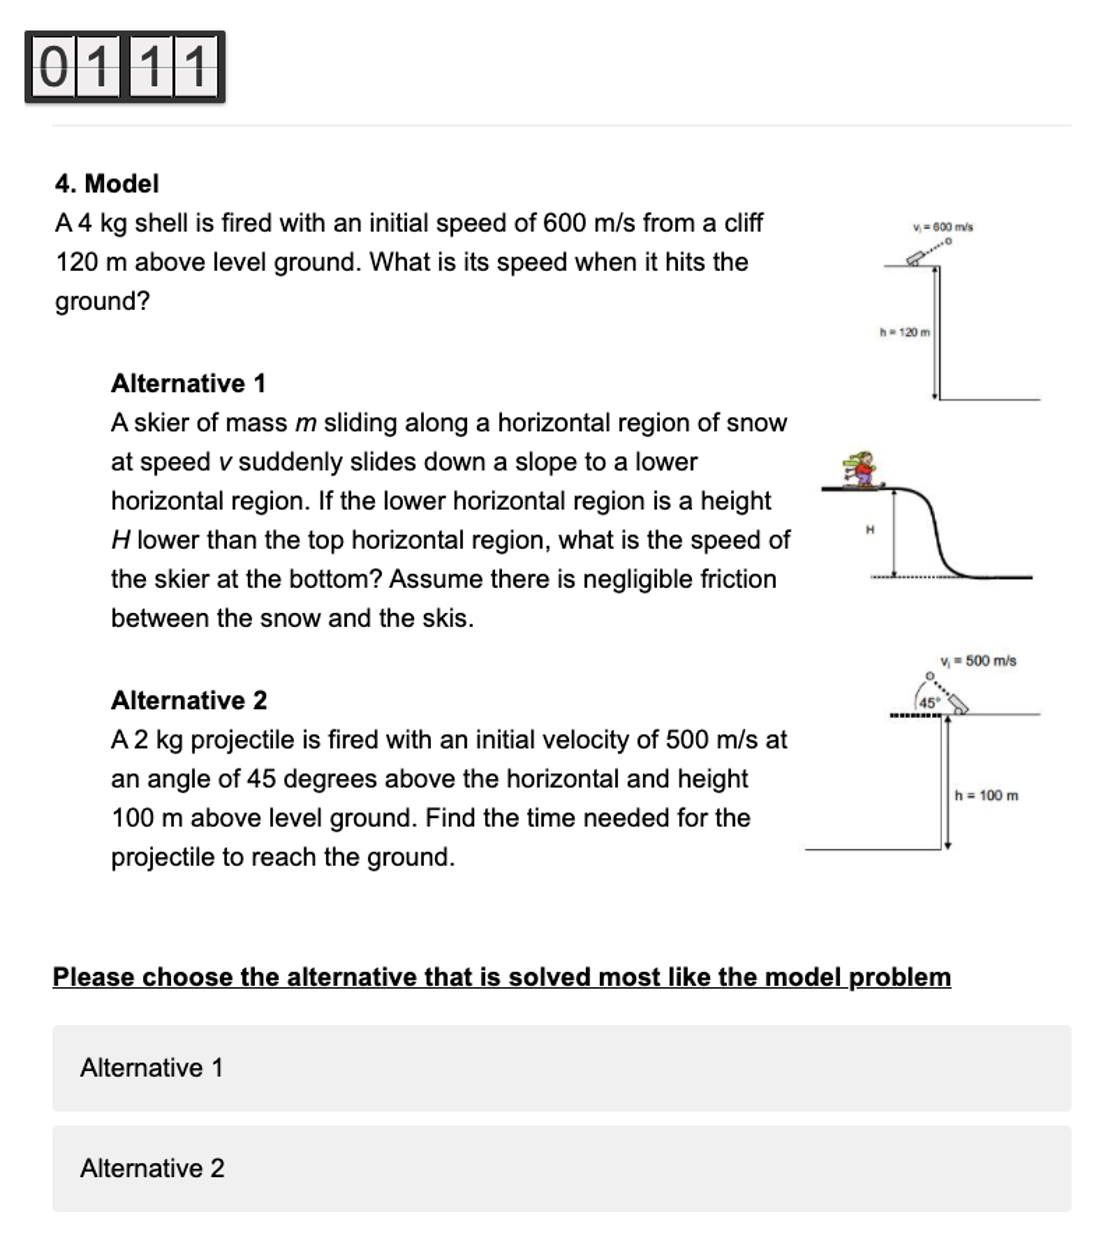
\includegraphics[width=0.75\linewidth,height=\textheight,keepaspectratio]{chapters/../img/sample-item-2.png}

}

\end{figure}%

\begin{tcolorbox}[enhanced jigsaw, bottomrule=.15mm, breakable, coltitle=black, rightrule=.15mm, colbacktitle=quarto-callout-note-color!10!white, leftrule=.75mm, titlerule=0mm, colframe=quarto-callout-note-color-frame, toprule=.15mm, colback=white, left=2mm, bottomtitle=1mm, opacitybacktitle=0.6, opacityback=0, toptitle=1mm, arc=.35mm, title=\textcolor{quarto-callout-note-color}{\faInfo}\hspace{0.5em}{Note}]

Supplementary Figure~\ref{fig-cat}: At first glance, the model problem
and alternative 2 appear similar because they both involve projectiles,
but this similarity is a surface-level distractor. The model problem and
alternative 1 are asking for final velocity and can be solved using
conservation of energy, while alternative 2 requires the use of
kinematics to solve for time. Therefore, the correct response is
alternative 1.

\end{tcolorbox}

\section{Physics Tasks, Part 3: Conceptual Questions (Qualitative
Problem
Solving)}\label{physics-tasks-part-3-conceptual-questions-qualitative-problem-solving}

This part consisted of three multiple-choice questions (See
Supplementary Figure~\ref{fig-qual-1}), followed by one open-ended
problem (See Supplementary Figure~\ref{fig-qual-2}). For each
multiple-choice question, participants were also asked to provide a
brief explanation for their choice. The open-ended problem was a word
problem in which participants were asked to explain a solution.

\begin{figure}

\begin{minipage}{0.50\linewidth}

\begin{figure}[H]

\caption{\label{fig-qual-1}Multiple-Choice Item}

\centering{

\pandocbounded{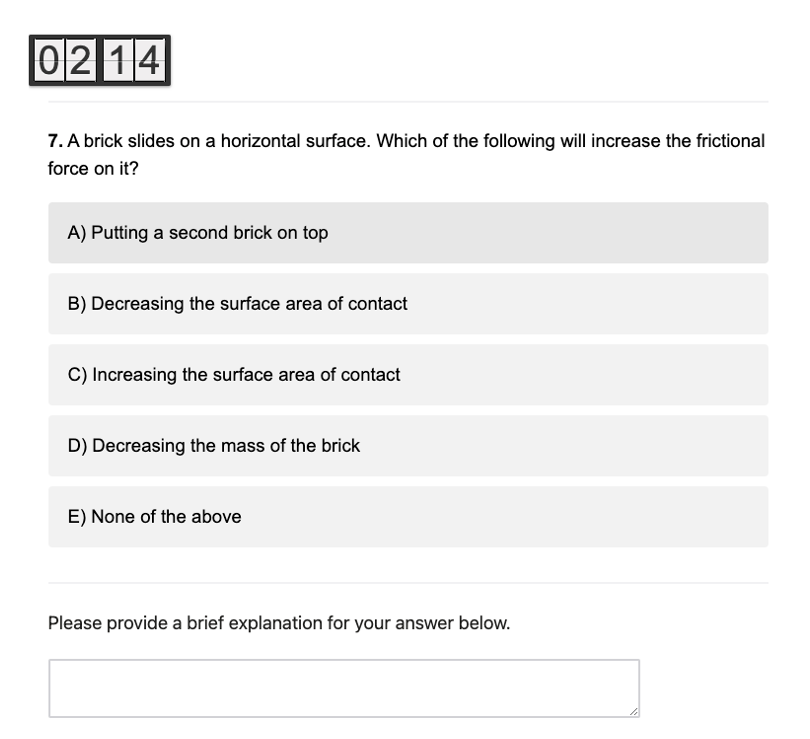
\includegraphics[keepaspectratio]{chapters/../img/sample-item-3.png}}

}

\end{figure}%

\end{minipage}%
%
\begin{minipage}{0.50\linewidth}

\begin{figure}[H]

\caption{\label{fig-qual-2}Open-Ended Item}

\centering{

\pandocbounded{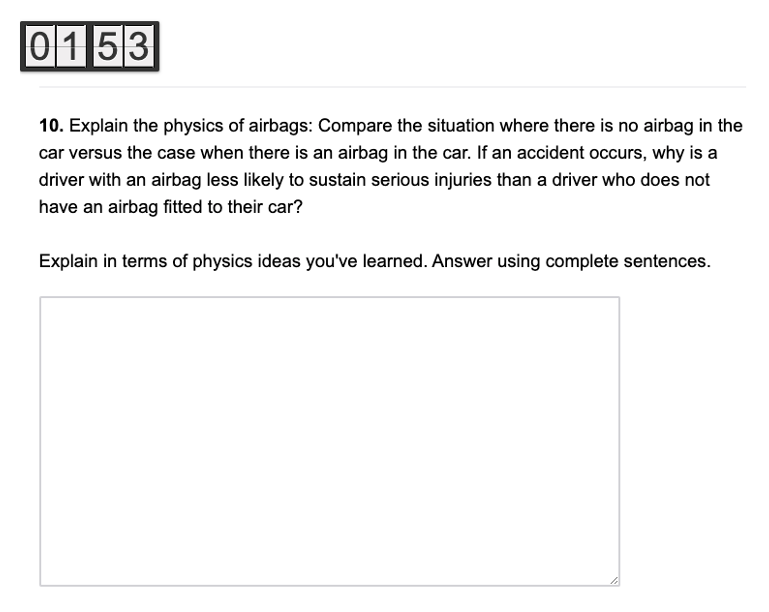
\includegraphics[keepaspectratio]{chapters/../img/sample-item-4.png}}

}

\end{figure}%

\end{minipage}%

\end{figure}%

\begin{tcolorbox}[enhanced jigsaw, bottomrule=.15mm, breakable, coltitle=black, rightrule=.15mm, colbacktitle=quarto-callout-note-color!10!white, leftrule=.75mm, titlerule=0mm, colframe=quarto-callout-note-color-frame, toprule=.15mm, colback=white, left=2mm, bottomtitle=1mm, opacitybacktitle=0.6, opacityback=0, toptitle=1mm, arc=.35mm, title=\textcolor{quarto-callout-note-color}{\faInfo}\hspace{0.5em}{Note}]

Supplementary Figure~\ref{fig-qual-1}: Qualitative multiple-choice item:
The correct answer is option A because the frictional force is
proportional to the normal force, which is equal to the weight force.
Therefore, the only way to increase the frictional force is to increase
the mass; Supplementary Figure~\ref{fig-qual-2}: Qualitative open
response item: Newton's second law states that
\(F_{net}=\frac{Δp}{Δt}\). Airbags reduce the force (outcome) of a
collision by increasing the time it takes for the collision to occur
(mechanism). Half credit was given to responses that mentioned either
force or time correctly, and full credit was given to responses that
mentioned both force and time.

\end{tcolorbox}

\section{Physics Tasks, Part 4: Preparation for Future
Learning}\label{physics-tasks-part-4-preparation-for-future-learning}

The Preparation for Future Learning (PFL) task (Belenky and Nokes-Malach
2012; Schwartz and Martin 2004) is a 3-part learning activity that
participants completed only at posttest. Physics problems used in the
learning activity were taken from Weinlader et al. (2019). The first
part consisted of solving a difficult multiple-choice problem which
required comparing the trajectories of two projectiles and predicting
which would hit their target first (see Supplementary
Figure~\ref{fig-pfl}). In the second part, a learning resource
explaining the first problem was provided. The resource contained an
explanation of why the correct answer choice was valid, and why each
incorrect answer was not. The third part consisted of a novel problem
with similar surface features to the first problem but had a different
correct response. Answering correctly required applying the underlying
principles of the first problem to a different set of conditions. Each
of the two problems required both a multiple-choice answer as well as a
short-answer explanation for the selected choice.

\begin{figure}[!hp]

\caption{\label{fig-pfl}Sample Preparation for Future Learning Task
Item}

\centering{

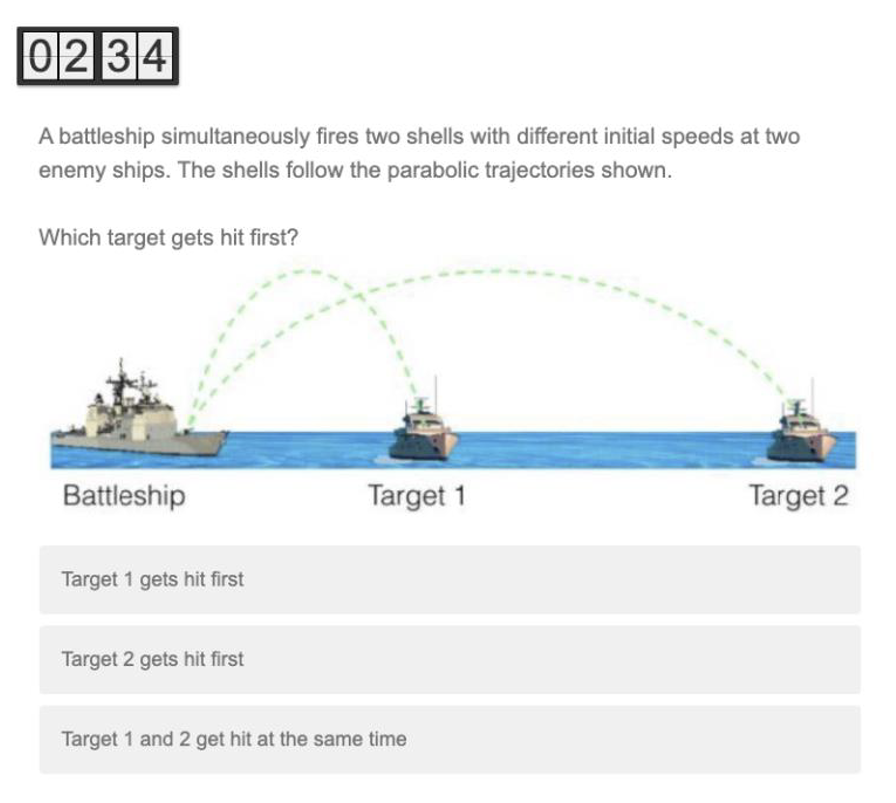
\includegraphics[width=0.75\linewidth,height=\textheight,keepaspectratio]{chapters/../img/sample-item-5.png}

}

\end{figure}%

\chapter{Scoring Procedure For Physics Learning and Performance
Outcomes}\label{scoring-procedure-for-physics-learning-and-performance-outcomes}

For all measures which required qualitative coding or scoring, the
following procedure was used: First, a rubric was developed through
group discussion with the research team. Then, a portion of the
responses were coded independently by a minimum of two coders.
Discrepancies from the first round of coding were reviewed by the team
and the rubric was revised as needed. The remaining responses were coded
again in full by two coders and all discrepancies were resolved in the
presence of a third coder. Any responses that could not be easily
resolved were brought to the research team for review. For each measure
that was coded or scored, we report two inter-rater reliability
statistics, one for each round of coding.

\section{Physics Assessment, Part 1: Quantitative Problem
Solving}\label{physics-assessment-part-1-quantitative-problem-solving}

The quantitative problems (one for each test version) were scored
according to a rubric developed by the research team. Partial credit was
given for incomplete or partially correct solutions. Responses from
baseline and posttest were combined and randomized within each test
version before scoring, and team members were blinded to condition. The
intraclass correlation for the first round of coding was .74 for version
A (20 responses) and .8 for version B (29 responses). The intraclass
correlation for the remaining solutions were .7 for version A (129
responses), and .94 for version B (117 responses). Final scores were
calculated by taking the proportion of points earned out of the total
possible points. Three responses on the posttest quantitative
problem-solving task were removed from analysis. In one case, it was
clear there was additional work cropped out of the uploaded image which
could not be scored; in another, the uploaded file was a duplicate of
their baseline file; and in the last case the handwriting was deemed
illegible by all of the raters.

\section{Physics Assessment, Part 2: Problem
Categorization}\label{physics-assessment-part-2-problem-categorization}

Individual items were scored dichotomously as 0 (incorrect) or 1
(correct). Final scores were calculated by taking the average accuracy
across the five categorization items.

\section{Physics Assessment, Part 3: Qualitative Problem
Solving}\label{physics-assessment-part-3-qualitative-problem-solving}

The three multiple-choice questions were scored dichotomously as 0
(incorrect) or 1 (correct). For the purposes of the current work and
questions we did not analyze the open-response explanations for the
multiple-choice questions. The open-ended word problem was coded and
scored by the research team. Responses were awarded a maximum of two
points: one point for each component of the correct explanation. For
example, the question in test version B described a scenario in which an
elevator cable snaps, and the emergency friction brakes are engaged. The
student was asked to describe the types of energy transfer which occur
in this scenario. One point was given for describing gravitational
potential energy being converted to kinetic energy, and another for
describing kinetic energy being converted to thermal and sound energy
due to work done by friction. Similar to the quantitative problem, all
responses were combined and randomized across timepoints, and
experimental condition was removed from the data before scoring. The
weighted Kappa for the first round of coding was .36 for version A (50
responses), and .58 for version B (53 responses). The weighted Kappas
for the second round of coding were .71 for version A (99 responses),
and .74 for version B (95 responses). When calculating the final score,
the open-ended word problem was weighted equal to the multiple-choice,
such that two-point responses were scored as a 1 and one-point responses
were scored as a .5. Final scores for qualitative problem solving were
calculated by taking the mean score of all the items.

\section{Physics Assessment, Part 4: Preparation for Future Learning
(PFL)}\label{physics-assessment-part-4-preparation-for-future-learning-pfl}

There were two components to the response for each of the two PFL
questions: multiple-choice selection and open-response explanation. We
defined correctness on the PFL as selecting the correct multiple choice
response option and reasoning correctly in the open-response
explanation. For both questions, student reasoning was considered
correct if they mentioned the relative maximum heights or initial
\emph{y} velocities of the two trajectories as a justification for their
answer, or if they mentioned that the \emph{y} component was most
important for determining time in the air. These questions were the only
ones for which we did not complete two separate rounds of coding because
we build directly on our past work with a similar population (Weinlader
et al. 2019). Otherwise, the coding procedure was identical to the
others. Responses were randomized and coders were blinded to condition.
Both PFL questions were coded in full by two coders as either correct or
incorrect. The unweighted Kappa for both of the PFL questions was .88.
All discrepancies were resolved through discussion in the presence of a
third coder.

\begin{table}

\caption{\label{tbl-scoring}Summary of Item Types and Scoring Scales by
Outcome}

\centering{

\centering\begingroup\fontsize{9}{11}\selectfont

\begin{tabular}[t]{>{\raggedright\arraybackslash}p{2.5in}>{\raggedright\arraybackslash}p{1.5in}>{\raggedright\arraybackslash}p{1.5in}}
\toprule
Outcome Measure & Items and Measurement & Scoring\\
\midrule
\addlinespace[0.3em]
\multicolumn{3}{l}{\textbf{Physics Problem Solving Performance}}\\
\hspace{1em}Part 1: Quantitative Problem Solving & 1 item, open response & Points earned/points possible, continuous from 0 to 1\\
\hspace{1em}Part 2: Problem Categorization & 5 items, forced-choice & Mean score, continuous from 0 to 1\\
\hspace{1em}Part 3: Qualitative Problem Solving & 3 multiple-choice, 1 open response & Mean score, continuous from 0 to 1\\
\addlinespace[0.3em]
\multicolumn{3}{l}{\textbf{Preparation for Future Learning}}\\
\hspace{1em}Part 4: Preparation for Future Learning & 2 items, multiple-choice with open response explanation & Dichotomous, 0 or 1: 1 = Correct multiple choice response \& attends to y component correctly in explanation\\
\addlinespace[0.3em]
\multicolumn{3}{l}{\textbf{Momentary Item-Level Perceptions}}\\
\hspace{1em}Confidence & 1 item, measured repeatedly & Continuous from 1 to 6\\
\hspace{1em}Anxiety & 1 item, measured repeatedly & Continuous from 1 to 6\\
\hspace{1em}Difficulty & 1 item, measured repeatedly & Continuous from 1 to 6\\
\bottomrule
\end{tabular}
\endgroup{}

}

\end{table}%

\chapter{Clustering Variables Examined but Not
Included}\label{clustering-variables-examined-but-not-included}

We explored the particular class section that the participants were
recruited from as a potential covariate. There were many aspects of the
classes that were homogeneous: all instructors were required to adhere
to the same set of pre-defined learning objectives, and beginning in
cohort 3's semester (during which over half our sample participated),
the department instituted measures which required classes to synchronize
exam schedules, recitation quizzes, homework systems, and textbooks.
Nevertheless, each class has its own variation in terms of the number of
students enrolled, days and times they meet, the amount of synchronous
vs.~asynchronous activities, and the students that select to be in those
classes. Furthermore, all instructors have idiosyncratic aspects to
their teaching methods and can have different demands and resources in
the class.~ The inclusion of class by instructor as a covariate was
explored, but ultimately not included. Seven instructors taught the
physics classes represented in our sample. Most instructors taught one
class except one instructor who taught two, and another who taught 4
(total of eleven classes).

The number of students associated with each class ranged from 5 to 21
(\emph{M} = 13.5, \emph{SD} = 5.01). Theoretically, it made sense to
include class and instructor as nested random intercept terms because we
wanted to account for clustering by class and instructor, but we did not
have any predictions about specific classes or professors. However, the
ICC for class and instructor was at or very close to zero in all the
models. This indicates that statistically, observations within classes
and instructors were no more similar to each other than to observations
from different classes and instructors. We also conducted a visual
inspection of the all the focal study variables by instructor and did
not detect any differences that appeared systematic. Based on these
analyses, we did not include class or instructor in the reported models.

\part{R Code and Analyses}

\chapter{Data and Environment Setup}\label{data-and-environment-setup}

\section{Source Setup Script}\label{source-setup-script}

In order to run the code included in this book, you first need to run
``/R/setup-script.R'' to install/load required packages and read the
data. The data are located in
``/data/preregistration\_3\_data\_public.csv''.

\section{Session Info}\label{session-info}

\begin{verbatim}
R version 4.5.0 (2025-04-11)
Platform: aarch64-apple-darwin20
Running under: macOS Sonoma 14.6.1

Matrix products: default
BLAS:   /Library/Frameworks/R.framework/Versions/4.5-arm64/Resources/lib/libRblas.0.dylib 
LAPACK: /Library/Frameworks/R.framework/Versions/4.5-arm64/Resources/lib/libRlapack.dylib;  LAPACK version 3.12.1

locale:
[1] en_US.UTF-8/en_US.UTF-8/en_US.UTF-8/C/en_US.UTF-8/en_US.UTF-8

time zone: America/New_York
tzcode source: internal

attached base packages:
[1] stats     graphics  grDevices utils     datasets  methods   base     

other attached packages:
 [1] lubridate_1.9.4    forcats_1.0.0      stringr_1.5.1      dplyr_1.1.4       
 [5] purrr_1.0.4        readr_2.1.5        tidyr_1.3.1        tibble_3.2.1      
 [9] tidyverse_2.0.0    ggpubr_0.6.0       rstatix_0.7.2      showtext_0.9-7    
[13] showtextdb_3.0     sysfonts_0.8.9     patchwork_1.3.0    GGally_2.2.1      
[17] ggplot2_3.5.2      sjtable2df_0.0.4   sjlabelled_1.2.0   sjmisc_2.8.10     
[21] sjPlot_2.8.17      lmerTest_3.1-3     lme4_1.1-37        mediation_4.5.0   
[25] sandwich_3.1-1     mvtnorm_1.3-3      Matrix_1.7-3       MASS_7.3-65       
[29] gvlma_1.0.0.3      performance_0.15.1 kableExtra_1.4.0   pacman_0.5.1      

loaded via a namespace (and not attached):
 [1] Rdpack_2.6.4        gridExtra_2.3       rlang_1.1.6        
 [4] magrittr_2.0.3      compiler_4.5.0      systemfonts_1.2.2  
 [7] vctrs_0.6.5         crayon_1.5.3        pkgconfig_2.0.3    
[10] fastmap_1.2.0       backports_1.5.0     rmarkdown_2.29     
[13] tzdb_0.5.0          nloptr_2.2.1        bit_4.6.0          
[16] xfun_0.52           jsonlite_2.0.0      ggeffects_2.2.1    
[19] parallel_4.5.0      broom_1.0.8         cluster_2.1.8.1    
[22] R6_2.6.1            stringi_1.8.7       RColorBrewer_1.1-3 
[25] car_3.1-3           boot_1.3-31         rpart_4.1.24       
[28] numDeriv_2016.8-1.1 Rcpp_1.0.14         knitr_1.50         
[31] zoo_1.8-14          base64enc_0.1-3     splines_4.5.0      
[34] nnet_7.3-20         timechange_0.3.0    tidyselect_1.2.1   
[37] rstudioapi_0.17.1   abind_1.4-8         yaml_2.3.10        
[40] codetools_0.2-20    curl_6.2.2          lattice_0.22-7     
[43] plyr_1.8.9          withr_3.0.2         evaluate_1.0.3     
[46] foreign_0.8-90      archive_1.1.12      ggstats_0.9.0      
[49] xml2_1.3.8          lpSolve_5.6.23      pillar_1.10.2      
[52] carData_3.0-5       checkmate_2.3.2     reformulas_0.4.0   
[55] insight_1.4.2       generics_0.1.3      vroom_1.6.5        
[58] hms_1.1.3           scales_1.4.0        minqa_1.2.8        
[61] glue_1.8.0          Hmisc_5.2-3         tools_4.5.0        
[64] data.table_1.17.8   ggsignif_0.6.4      grid_4.5.0         
[67] rbibutils_2.3       datawizard_1.2.0    colorspace_2.1-1   
[70] nlme_3.1-168        htmlTable_2.4.3     Formula_1.2-5      
[73] cli_3.6.5           viridisLite_0.4.2   svglite_2.1.3      
[76] sjstats_0.19.0      gtable_0.3.6        digest_0.6.37      
[79] htmlwidgets_1.6.4   farver_2.1.2        htmltools_0.5.8.1  
[82] lifecycle_1.0.4     bit64_4.6.0-1      
\end{verbatim}

\section{Datasets}\label{datasets}

The analyses in the main text are run using two forms of the data, one
for each research question / analysis type. Summaries of the data
charactaristics are described below.

\subsection{RQ1 Data}\label{rq1-data}

These data are in long format - (22 items x 149 participants - 3 NA
values) x 3 judgments per item = 9825 observations.

\begin{tcolorbox}[enhanced jigsaw, bottomrule=.15mm, breakable, coltitle=black, rightrule=.15mm, colbacktitle=quarto-callout-note-color!10!white, leftrule=.75mm, titlerule=0mm, colframe=quarto-callout-note-color-frame, toprule=.15mm, colback=white, left=2mm, bottomtitle=1mm, opacitybacktitle=0.6, opacityback=0, toptitle=1mm, arc=.35mm, title=\textcolor{quarto-callout-note-color}{\faInfo}\hspace{0.5em}{Note}]

the variable \texttt{perception} is equivalent to ``judgment'' in the
manuscript.

\end{tcolorbox}

\begin{verbatim}
Rows: 9,825
Columns: 17
$ Participant           <chr> "mvU3yT4uTFpW58Z0", "mvU3yT4uTFpW58Z0", "mvU3yT4~
$ Condition             <fct> Control, Control, Control, Control, Control, Con~
$ Gender                <fct> Men, Men, Men, Men, Men, Men, Men, Men, Men, Men~
$ Cohort                <fct> Cohort 1, Cohort 1, Cohort 1, Cohort 1, Cohort 1~
$ Timepoint             <fct> Baseline, Baseline, Baseline, Baseline, Baseline~
$ Semester_Week         <dbl> 1.912752, 1.912752, 1.912752, 1.912752, 1.912752~
$ Test_Version          <fct> B, B, B, B, B, B, B, B, B, B, B, B, B, B, B, B, ~
$ Part                  <chr> "Quantitative", "Quantitative", "Quantitative", ~
$ Question              <dbl> 1, 1, 1, 2, 2, 2, 3, 3, 3, 4, 4, 4, 5, 5, 5, 6, ~
$ Item                  <chr> "B01", "B01", "B01", "B02", "B02", "B02", "B03",~
$ Score                 <dbl> 0, 0, 0, 0, 0, 0, 1, 1, 1, 0, 0, 0, 0, 0, 0, 0, ~
$ `Item-Level Accuracy` <fct> Incorrect, Incorrect, Incorrect, Incorrect, Inco~
$ Accuracy_Raw          <dbl> 0, 0, 0, 0, 0, 0, 1, 1, 1, 0, 0, 0, 0, 0, 0, 0, ~
$ Baseline_Threat       <dbl> 1.63132, 1.63132, 1.63132, 1.63132, 1.63132, 1.6~
$ EMA_Threat            <dbl> 3.416667, 3.416667, 3.416667, 3.416667, 3.416667~
$ perception            <fct> Confidence, Anxiety, Difficulty, Confidence, Anx~
$ rating                <dbl> 1, 6, 6, 5, 6, 2, 4, 6, 3, 5, 6, 4, 5, 6, 4, 4, ~
\end{verbatim}

\subsubsection{Participant-Level
Variables}\label{participant-level-variables}

\begin{verbatim}
 Participant              Condition                  Gender        Cohort  
 Length:149         Control    :73   Men                :66   Cohort 1:61  
 Class :character   Mindfulness:76   Women or Non-binary:83   Cohort 2:16  
 Mode  :character                                             Cohort 3:72  
\end{verbatim}

\begin{longtable}[]{@{}lrrrrr@{}}
\toprule\noalign{}
variable & n & min & max & mean & sd \\
\midrule\noalign{}
\endhead
\bottomrule\noalign{}
\endlastfoot
Semester\_Week & 149 & -4.087 & 4.913 & 0 & 2.790 \\
Baseline\_Threat & 149 & -3.102 & 2.865 & 0 & 1.297 \\
\end{longtable}

\subsubsection{Item (Observation)-Level
Variables}\label{item-observation-level-variables}

\begin{tcolorbox}[enhanced jigsaw, bottomrule=.15mm, breakable, coltitle=black, rightrule=.15mm, colbacktitle=quarto-callout-note-color!10!white, leftrule=.75mm, titlerule=0mm, colframe=quarto-callout-note-color-frame, toprule=.15mm, colback=white, left=2mm, bottomtitle=1mm, opacitybacktitle=0.6, opacityback=0, toptitle=1mm, arc=.35mm, title=\textcolor{quarto-callout-note-color}{\faInfo}\hspace{0.5em}{Note}]

\texttt{Score} includes values between 0 and 1 since 4 of the items
(A01, B01, A10, and B10) were open-ended and could be awarded partial
credit. \texttt{Item-Level\ Accuracy} (factor version) and
\texttt{Accuracy\_Raw} (numeric version) were derived from
\texttt{Score} to compare incorrect responses to those that were at
least partially correct (\texttt{Score} \textgreater{} 0).

\end{tcolorbox}

\begin{verbatim}
     Item              Timepoint    Test_Version Item-Level Accuracy
 Length:9825        Baseline:4470   A:4908       Incorrect:5547     
 Class :character   Posttest:5355   B:4917       Correct  :4278     
 Mode  :character                                                   
      perception  
 Confidence:3275  
 Anxiety   :3275  
 Difficulty:3275  
\end{verbatim}

\begin{longtable}[]{@{}lrrrrr@{}}
\toprule\noalign{}
variable & n & min & max & mean & sd \\
\midrule\noalign{}
\endhead
\bottomrule\noalign{}
\endlastfoot
Score & 9825 & 0 & 1 & 0.404 & 0.478 \\
Accuracy\_Raw & 9825 & 0 & 1 & 0.435 & 0.496 \\
rating & 9825 & 1 & 6 & 3.474 & 1.408 \\
\end{longtable}

\subsection{RQ2 Data}\label{rq2-data}

Data are in wide format, so everything varies at the participant level.
Judgment ratings and accuracy scores are averaged at baseline and
posttest. Continuous variables are standardized and numeric dummy
variables with contrast coding are created for \texttt{Cohort} because
the \texttt{mediation} package does not accept factors with contrast
coding, but this has no bearing on the results. One participant's data
was removed because they did not complete any EMA surveys.

\begin{verbatim}
Rows: 148
Columns: 21
$ Participant           <chr> "mvU3yT4uTFpW58Z0", "bTvjXPvFUSNyAt5t", "hx3UKKU~
$ Condition             <fct> Control, Control, Control, Control, Control, Con~
$ Gender                <fct> Men, Men, Men, Women or Non-binary, Men, Women o~
$ Cohort                <fct> Cohort 1, Cohort 1, Cohort 1, Cohort 1, Cohort 3~
$ Semester_Week         <dbl> 0.6786886, 0.6786886, 0.6786886, 1.0374240, -0.7~
$ Baseline_Threat       <dbl> 1.25100904, -0.75116043, -1.05918650, 1.89273003~
$ EMA_Threat            <dbl> 1.55096412, 1.29550795, -0.95250627, 1.29550795,~
$ Baseline_n_items      <int> 10, 10, 10, 10, 10, 10, 10, 10, 10, 10, 10, 10, ~
$ Posttest_n_items      <int> 12, 12, 12, 12, 12, 12, 11, 12, 12, 12, 12, 12, ~
$ Baseline_Score        <dbl> -0.31125932, 0.33654914, -0.49120612, -1.6068762~
$ Posttest_Score        <dbl> -1.34709242, 1.43972775, -0.78972839, -2.4618204~
$ Baseline_Confidence   <dbl> -0.37485943, 0.01220473, 0.39926888, -2.18115882~
$ Posttest_Confidence   <dbl> 0.23891063, 0.53917812, 0.53917812, -3.36429935,~
$ Baseline_Anxiety      <dbl> 2.49202355, -0.85159304, -0.57295832, 1.65611940~
$ Posttest_Anxiety      <dbl> 2.15254688, -0.25189270, -0.99809809, 2.40128201~
$ Baseline_Difficulty   <dbl> 1.15470752, -1.16207408, -0.20810518, 2.24495769~
$ Posttest_Difficulty   <dbl> 1.4257825, -0.7405502, -0.0184393, 2.4573694, 0.~
$ Baseline_Test_Version <chr> "B", "A", "B", "A", "B", "A", "A", "B", "A", "A"~
$ Posttest_Test_Version <fct> A, B, A, B, A, B, B, A, B, B, A, B, B, B, B, B, ~
$ Cohort_2              <dbl> -0.3469771, -0.3469771, -0.3469771, -0.3469771, ~
$ Cohort_3              <dbl> -0.9569993, -0.9569993, -0.9569993, -0.9569993, ~
\end{verbatim}

\begin{verbatim}
 Participant              Condition                  Gender        Cohort  
 Length:148         Control    :73   Men                :66   Cohort 1:61  
 Class :character   Mindfulness:75   Women or Non-binary:82   Cohort 2:16  
 Mode  :character                                             Cohort 3:71  
 Baseline_Test_Version Posttest_Test_Version
 A:75                  A:73                 
 B:73                  B:75                 
                                            
\end{verbatim}

\begin{longtable}[]{@{}lrrrrr@{}}
\toprule\noalign{}
variable & n & min & max & mean & sd \\
\midrule\noalign{}
\endhead
\bottomrule\noalign{}
\endlastfoot
Semester\_Week & 148 & -1.474 & 1.755 & 0.00 & 1.000 \\
Baseline\_Threat & 148 & -2.394 & 2.201 & 0.00 & 1.000 \\
EMA\_Threat & 148 & -2.230 & 2.420 & 0.00 & 1.000 \\
Baseline\_n\_items & 148 & 10.000 & 10.000 & 10.00 & 0.000 \\
Posttest\_n\_items & 148 & 11.000 & 12.000 & 11.98 & 0.141 \\
Baseline\_Score & 148 & -2.111 & 3.511 & 0.00 & 1.000 \\
Posttest\_Score & 148 & -2.462 & 2.957 & 0.00 & 1.000 \\
Baseline\_Confidence & 148 & -3.213 & 2.206 & 0.00 & 1.000 \\
Posttest\_Confidence & 148 & -3.464 & 1.840 & 0.00 & 1.000 \\
Baseline\_Anxiety & 148 & -2.152 & 2.492 & 0.00 & 1.000 \\
Posttest\_Anxiety & 148 & -1.993 & 2.650 & 0.00 & 1.000 \\
Baseline\_Difficulty & 148 & -2.389 & 2.381 & 0.00 & 1.000 \\
Posttest\_Difficulty & 148 & -2.701 & 2.457 & 0.00 & 1.000 \\
Cohort\_2 & 148 & -0.347 & 2.863 & 0.00 & 1.000 \\
Cohort\_3 & 148 & -0.957 & 1.038 & 0.00 & 1.000 \\
\end{longtable}

\chapter{Characteristics of Fixed Effects Variables for Mixed
Models}\label{characteristics-of-fixed-effects-variables-for-mixed-models}

The following code reproduces the factor coding and descriptive
statistics reported in Table 3 of the main text.

\section{Dependent Variables}\label{dependent-variables}

\subsubsection{Confidence}\label{confidence}

\begin{longtable}[]{@{}
  >{\raggedright\arraybackslash}p{(\linewidth - 20\tabcolsep) * \real{0.1538}}
  >{\raggedright\arraybackslash}p{(\linewidth - 20\tabcolsep) * \real{0.1385}}
  >{\raggedleft\arraybackslash}p{(\linewidth - 20\tabcolsep) * \real{0.0769}}
  >{\raggedleft\arraybackslash}p{(\linewidth - 20\tabcolsep) * \real{0.0615}}
  >{\raggedleft\arraybackslash}p{(\linewidth - 20\tabcolsep) * \real{0.0615}}
  >{\raggedleft\arraybackslash}p{(\linewidth - 20\tabcolsep) * \real{0.1077}}
  >{\raggedleft\arraybackslash}p{(\linewidth - 20\tabcolsep) * \real{0.0615}}
  >{\raggedright\arraybackslash}p{(\linewidth - 20\tabcolsep) * \real{0.0769}}
  >{\raggedright\arraybackslash}p{(\linewidth - 20\tabcolsep) * \real{0.0769}}
  >{\raggedleft\arraybackslash}p{(\linewidth - 20\tabcolsep) * \real{0.0923}}
  >{\raggedleft\arraybackslash}p{(\linewidth - 20\tabcolsep) * \real{0.0923}}@{}}
\toprule\noalign{}
\begin{minipage}[b]{\linewidth}\raggedright
Timepoint
\end{minipage} & \begin{minipage}[b]{\linewidth}\raggedright
variable
\end{minipage} & \begin{minipage}[b]{\linewidth}\raggedleft
n
\end{minipage} & \begin{minipage}[b]{\linewidth}\raggedleft
min
\end{minipage} & \begin{minipage}[b]{\linewidth}\raggedleft
max
\end{minipage} & \begin{minipage}[b]{\linewidth}\raggedleft
median
\end{minipage} & \begin{minipage}[b]{\linewidth}\raggedleft
iqr
\end{minipage} & \begin{minipage}[b]{\linewidth}\raggedright
mean
\end{minipage} & \begin{minipage}[b]{\linewidth}\raggedright
sd
\end{minipage} & \begin{minipage}[b]{\linewidth}\raggedleft
se
\end{minipage} & \begin{minipage}[b]{\linewidth}\raggedleft
ci
\end{minipage} \\
\midrule\noalign{}
\endhead
\bottomrule\noalign{}
\endlastfoot
Baseline & rating & 1490 & 1 & 6 & 4 & 2 & 3.69 & 1.44 & 0.037 &
0.073 \\
Posttest & rating & 1785 & 1 & 6 & 4 & 2 & 3.88 & 1.46 & 0.035 &
0.068 \\
\end{longtable}

\subsubsection{Anxiety}\label{anxiety}

\begin{longtable}[]{@{}
  >{\raggedright\arraybackslash}p{(\linewidth - 20\tabcolsep) * \real{0.1538}}
  >{\raggedright\arraybackslash}p{(\linewidth - 20\tabcolsep) * \real{0.1385}}
  >{\raggedleft\arraybackslash}p{(\linewidth - 20\tabcolsep) * \real{0.0769}}
  >{\raggedleft\arraybackslash}p{(\linewidth - 20\tabcolsep) * \real{0.0615}}
  >{\raggedleft\arraybackslash}p{(\linewidth - 20\tabcolsep) * \real{0.0615}}
  >{\raggedleft\arraybackslash}p{(\linewidth - 20\tabcolsep) * \real{0.1077}}
  >{\raggedleft\arraybackslash}p{(\linewidth - 20\tabcolsep) * \real{0.0615}}
  >{\raggedright\arraybackslash}p{(\linewidth - 20\tabcolsep) * \real{0.0769}}
  >{\raggedright\arraybackslash}p{(\linewidth - 20\tabcolsep) * \real{0.0769}}
  >{\raggedleft\arraybackslash}p{(\linewidth - 20\tabcolsep) * \real{0.0923}}
  >{\raggedleft\arraybackslash}p{(\linewidth - 20\tabcolsep) * \real{0.0923}}@{}}
\toprule\noalign{}
\begin{minipage}[b]{\linewidth}\raggedright
Timepoint
\end{minipage} & \begin{minipage}[b]{\linewidth}\raggedright
variable
\end{minipage} & \begin{minipage}[b]{\linewidth}\raggedleft
n
\end{minipage} & \begin{minipage}[b]{\linewidth}\raggedleft
min
\end{minipage} & \begin{minipage}[b]{\linewidth}\raggedleft
max
\end{minipage} & \begin{minipage}[b]{\linewidth}\raggedleft
median
\end{minipage} & \begin{minipage}[b]{\linewidth}\raggedleft
iqr
\end{minipage} & \begin{minipage}[b]{\linewidth}\raggedright
mean
\end{minipage} & \begin{minipage}[b]{\linewidth}\raggedright
sd
\end{minipage} & \begin{minipage}[b]{\linewidth}\raggedleft
se
\end{minipage} & \begin{minipage}[b]{\linewidth}\raggedleft
ci
\end{minipage} \\
\midrule\noalign{}
\endhead
\bottomrule\noalign{}
\endlastfoot
Baseline & rating & 1490 & 1 & 6 & 3 & 2 & 3.31 & 1.41 & 0.036 &
0.071 \\
Posttest & rating & 1785 & 1 & 6 & 3 & 2 & 3.00 & 1.37 & 0.033 &
0.064 \\
\end{longtable}

\subsubsection{Difficulty}\label{difficulty}

\begin{longtable}[]{@{}
  >{\raggedright\arraybackslash}p{(\linewidth - 20\tabcolsep) * \real{0.1538}}
  >{\raggedright\arraybackslash}p{(\linewidth - 20\tabcolsep) * \real{0.1385}}
  >{\raggedleft\arraybackslash}p{(\linewidth - 20\tabcolsep) * \real{0.0769}}
  >{\raggedleft\arraybackslash}p{(\linewidth - 20\tabcolsep) * \real{0.0615}}
  >{\raggedleft\arraybackslash}p{(\linewidth - 20\tabcolsep) * \real{0.0615}}
  >{\raggedleft\arraybackslash}p{(\linewidth - 20\tabcolsep) * \real{0.1077}}
  >{\raggedleft\arraybackslash}p{(\linewidth - 20\tabcolsep) * \real{0.0615}}
  >{\raggedright\arraybackslash}p{(\linewidth - 20\tabcolsep) * \real{0.0769}}
  >{\raggedright\arraybackslash}p{(\linewidth - 20\tabcolsep) * \real{0.0769}}
  >{\raggedleft\arraybackslash}p{(\linewidth - 20\tabcolsep) * \real{0.0923}}
  >{\raggedleft\arraybackslash}p{(\linewidth - 20\tabcolsep) * \real{0.0923}}@{}}
\toprule\noalign{}
\begin{minipage}[b]{\linewidth}\raggedright
Timepoint
\end{minipage} & \begin{minipage}[b]{\linewidth}\raggedright
variable
\end{minipage} & \begin{minipage}[b]{\linewidth}\raggedleft
n
\end{minipage} & \begin{minipage}[b]{\linewidth}\raggedleft
min
\end{minipage} & \begin{minipage}[b]{\linewidth}\raggedleft
max
\end{minipage} & \begin{minipage}[b]{\linewidth}\raggedleft
median
\end{minipage} & \begin{minipage}[b]{\linewidth}\raggedleft
iqr
\end{minipage} & \begin{minipage}[b]{\linewidth}\raggedright
mean
\end{minipage} & \begin{minipage}[b]{\linewidth}\raggedright
sd
\end{minipage} & \begin{minipage}[b]{\linewidth}\raggedleft
se
\end{minipage} & \begin{minipage}[b]{\linewidth}\raggedleft
ci
\end{minipage} \\
\midrule\noalign{}
\endhead
\bottomrule\noalign{}
\endlastfoot
Baseline & rating & 1490 & 1 & 6 & 4 & 1 & 3.55 & 1.26 & 0.033 &
0.064 \\
Posttest & rating & 1785 & 1 & 6 & 4 & 2 & 3.43 & 1.30 & 0.031 &
0.060 \\
\end{longtable}

\section{Covariates}\label{covariates}

\subsection{Cohort}\label{cohort}

\begin{longtable}[]{@{}lll@{}}
\toprule\noalign{}
Factor Levels & Cohort 2 & Cohort 3 \\
\midrule\noalign{}
\endhead
\bottomrule\noalign{}
\endlastfoot
Cohort 1 & -0.11 & -0.48 \\
Cohort 2 & 0.89 & -0.48 \\
Cohort 3 & -0.11 & 0.52 \\
\end{longtable}

\subsection{Semester Week}\label{semester-week}

\begin{longtable}[]{@{}
  >{\raggedright\arraybackslash}p{(\linewidth - 18\tabcolsep) * \real{0.2188}}
  >{\raggedleft\arraybackslash}p{(\linewidth - 18\tabcolsep) * \real{0.0625}}
  >{\raggedleft\arraybackslash}p{(\linewidth - 18\tabcolsep) * \real{0.1094}}
  >{\raggedleft\arraybackslash}p{(\linewidth - 18\tabcolsep) * \real{0.0938}}
  >{\raggedleft\arraybackslash}p{(\linewidth - 18\tabcolsep) * \real{0.1094}}
  >{\raggedleft\arraybackslash}p{(\linewidth - 18\tabcolsep) * \real{0.0625}}
  >{\raggedleft\arraybackslash}p{(\linewidth - 18\tabcolsep) * \real{0.0781}}
  >{\raggedleft\arraybackslash}p{(\linewidth - 18\tabcolsep) * \real{0.0781}}
  >{\raggedleft\arraybackslash}p{(\linewidth - 18\tabcolsep) * \real{0.0938}}
  >{\raggedleft\arraybackslash}p{(\linewidth - 18\tabcolsep) * \real{0.0938}}@{}}
\toprule\noalign{}
\begin{minipage}[b]{\linewidth}\raggedright
variable
\end{minipage} & \begin{minipage}[b]{\linewidth}\raggedleft
n
\end{minipage} & \begin{minipage}[b]{\linewidth}\raggedleft
min
\end{minipage} & \begin{minipage}[b]{\linewidth}\raggedleft
max
\end{minipage} & \begin{minipage}[b]{\linewidth}\raggedleft
median
\end{minipage} & \begin{minipage}[b]{\linewidth}\raggedleft
iqr
\end{minipage} & \begin{minipage}[b]{\linewidth}\raggedleft
mean
\end{minipage} & \begin{minipage}[b]{\linewidth}\raggedleft
sd
\end{minipage} & \begin{minipage}[b]{\linewidth}\raggedleft
se
\end{minipage} & \begin{minipage}[b]{\linewidth}\raggedleft
ci
\end{minipage} \\
\midrule\noalign{}
\endhead
\bottomrule\noalign{}
\endlastfoot
Semester\_Week & 149 & -4.087 & 4.913 & -1.087 & 5 & 0 & 2.79 & 0.229 &
0.452 \\
\end{longtable}

\subsection{Test Version}\label{test-version}

\begin{longtable}[]{@{}ll@{}}
\toprule\noalign{}
Factor Levels & B \\
\midrule\noalign{}
\endhead
\bottomrule\noalign{}
\endlastfoot
A & -0.50 \\
B & 0.50 \\
\end{longtable}

\subsection{Item-Level Accuracy}\label{item-level-accuracy}

Factor Coding:

\begin{longtable}[]{@{}ll@{}}
\toprule\noalign{}
Factor Levels & Correct \\
\midrule\noalign{}
\endhead
\bottomrule\noalign{}
\endlastfoot
Incorrect & -0.44 \\
Correct & 0.56 \\
\end{longtable}

Baseline and Posttest Means and Standard Deviations:

\begin{longtable}[]{@{}
  >{\raggedright\arraybackslash}p{(\linewidth - 20\tabcolsep) * \real{0.1449}}
  >{\raggedright\arraybackslash}p{(\linewidth - 20\tabcolsep) * \real{0.1884}}
  >{\raggedleft\arraybackslash}p{(\linewidth - 20\tabcolsep) * \real{0.0725}}
  >{\raggedleft\arraybackslash}p{(\linewidth - 20\tabcolsep) * \real{0.0580}}
  >{\raggedleft\arraybackslash}p{(\linewidth - 20\tabcolsep) * \real{0.0580}}
  >{\raggedleft\arraybackslash}p{(\linewidth - 20\tabcolsep) * \real{0.1014}}
  >{\raggedleft\arraybackslash}p{(\linewidth - 20\tabcolsep) * \real{0.0580}}
  >{\raggedright\arraybackslash}p{(\linewidth - 20\tabcolsep) * \real{0.0725}}
  >{\raggedright\arraybackslash}p{(\linewidth - 20\tabcolsep) * \real{0.0725}}
  >{\raggedleft\arraybackslash}p{(\linewidth - 20\tabcolsep) * \real{0.0870}}
  >{\raggedleft\arraybackslash}p{(\linewidth - 20\tabcolsep) * \real{0.0870}}@{}}
\toprule\noalign{}
\begin{minipage}[b]{\linewidth}\raggedright
Timepoint
\end{minipage} & \begin{minipage}[b]{\linewidth}\raggedright
variable
\end{minipage} & \begin{minipage}[b]{\linewidth}\raggedleft
n
\end{minipage} & \begin{minipage}[b]{\linewidth}\raggedleft
min
\end{minipage} & \begin{minipage}[b]{\linewidth}\raggedleft
max
\end{minipage} & \begin{minipage}[b]{\linewidth}\raggedleft
median
\end{minipage} & \begin{minipage}[b]{\linewidth}\raggedleft
iqr
\end{minipage} & \begin{minipage}[b]{\linewidth}\raggedright
mean
\end{minipage} & \begin{minipage}[b]{\linewidth}\raggedright
sd
\end{minipage} & \begin{minipage}[b]{\linewidth}\raggedleft
se
\end{minipage} & \begin{minipage}[b]{\linewidth}\raggedleft
ci
\end{minipage} \\
\midrule\noalign{}
\endhead
\bottomrule\noalign{}
\endlastfoot
Baseline & Accuracy\_Raw & 1490 & 0 & 1 & 0 & 1 & 0.43 & 0.50 & 0.013 &
0.025 \\
Posttest & Accuracy\_Raw & 1785 & 0 & 1 & 0 & 1 & 0.44 & 0.50 & 0.012 &
0.023 \\
\end{longtable}

\subsection{Baseline Threat}\label{baseline-threat}

\begin{longtable}[]{@{}
  >{\raggedright\arraybackslash}p{(\linewidth - 18\tabcolsep) * \real{0.2353}}
  >{\raggedleft\arraybackslash}p{(\linewidth - 18\tabcolsep) * \real{0.0588}}
  >{\raggedleft\arraybackslash}p{(\linewidth - 18\tabcolsep) * \real{0.1029}}
  >{\raggedleft\arraybackslash}p{(\linewidth - 18\tabcolsep) * \real{0.0882}}
  >{\raggedleft\arraybackslash}p{(\linewidth - 18\tabcolsep) * \real{0.1029}}
  >{\raggedleft\arraybackslash}p{(\linewidth - 18\tabcolsep) * \real{0.0882}}
  >{\raggedleft\arraybackslash}p{(\linewidth - 18\tabcolsep) * \real{0.0735}}
  >{\raggedleft\arraybackslash}p{(\linewidth - 18\tabcolsep) * \real{0.0882}}
  >{\raggedleft\arraybackslash}p{(\linewidth - 18\tabcolsep) * \real{0.0882}}
  >{\raggedleft\arraybackslash}p{(\linewidth - 18\tabcolsep) * \real{0.0735}}@{}}
\toprule\noalign{}
\begin{minipage}[b]{\linewidth}\raggedright
variable
\end{minipage} & \begin{minipage}[b]{\linewidth}\raggedleft
n
\end{minipage} & \begin{minipage}[b]{\linewidth}\raggedleft
min
\end{minipage} & \begin{minipage}[b]{\linewidth}\raggedleft
max
\end{minipage} & \begin{minipage}[b]{\linewidth}\raggedleft
median
\end{minipage} & \begin{minipage}[b]{\linewidth}\raggedleft
iqr
\end{minipage} & \begin{minipage}[b]{\linewidth}\raggedleft
mean
\end{minipage} & \begin{minipage}[b]{\linewidth}\raggedleft
sd
\end{minipage} & \begin{minipage}[b]{\linewidth}\raggedleft
se
\end{minipage} & \begin{minipage}[b]{\linewidth}\raggedleft
ci
\end{minipage} \\
\midrule\noalign{}
\endhead
\bottomrule\noalign{}
\endlastfoot
Baseline\_Threat & 149 & -3.102 & 2.865 & -0.035 & 1.933 & 0 & 1.297 &
0.106 & 0.21 \\
\end{longtable}

\section{Main Independent Variables of
Interest}\label{main-independent-variables-of-interest}

\subsection{Timepoint}\label{timepoint}

\begin{longtable}[]{@{}lr@{}}
\toprule\noalign{}
Factor Levels & Posttest \\
\midrule\noalign{}
\endhead
\bottomrule\noalign{}
\endlastfoot
Baseline & 0 \\
Posttest & 1 \\
\end{longtable}

\subsection{Condition}\label{condition}

\begin{longtable}[]{@{}lr@{}}
\toprule\noalign{}
Factor Levels & Mindfulness \\
\midrule\noalign{}
\endhead
\bottomrule\noalign{}
\endlastfoot
Control & -0.5 \\
Mindfulness & 0.5 \\
\end{longtable}

\subsection{Gender}\label{gender}

\begin{longtable}[]{@{}ll@{}}
\toprule\noalign{}
Factor Levels & Women or Non-binary \\
\midrule\noalign{}
\endhead
\bottomrule\noalign{}
\endlastfoot
Men & -0.56 \\
Women or Non-binary & 0.44 \\
\end{longtable}

\chapter{Correlations of Variables at
Baseline}\label{correlations-of-variables-at-baseline}

\section{Reproduction of Figure 3}\label{reproduction-of-figure-3}

\begin{figure}[!hp]

\caption{\label{fig-main-fig-3}Correlations and Variable Distributions
at Baseline (Main Text, Figure 3)}

\centering{

\pandocbounded{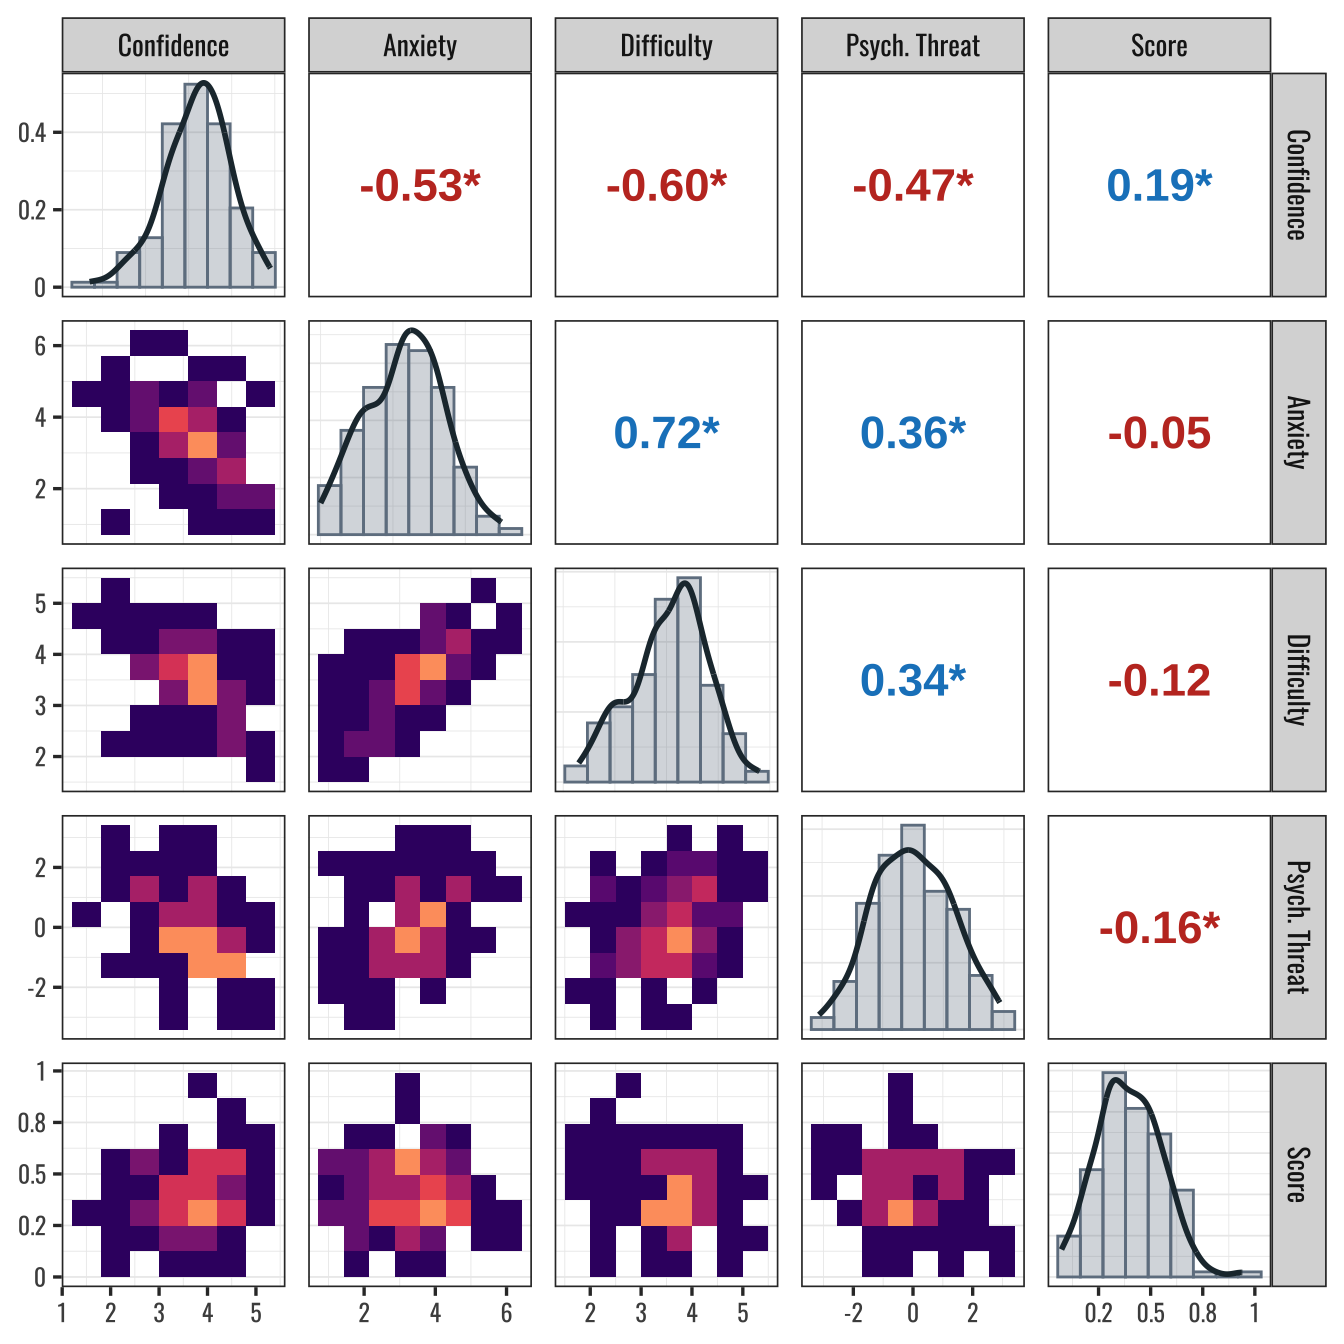
\includegraphics[keepaspectratio]{chapters/07-baseline-correlations_files/figure-pdf/fig-main-fig-3-1.pdf}}

}

\end{figure}%

\section{Association Between Item-Level Judgments by
Task}\label{association-between-item-level-judgments-by-task}

\begin{figure}[!hp]

\caption{\label{fig-judgment-by-task}Mean Judgments by Physics Task Type
at Baseline}

\centering{

\pandocbounded{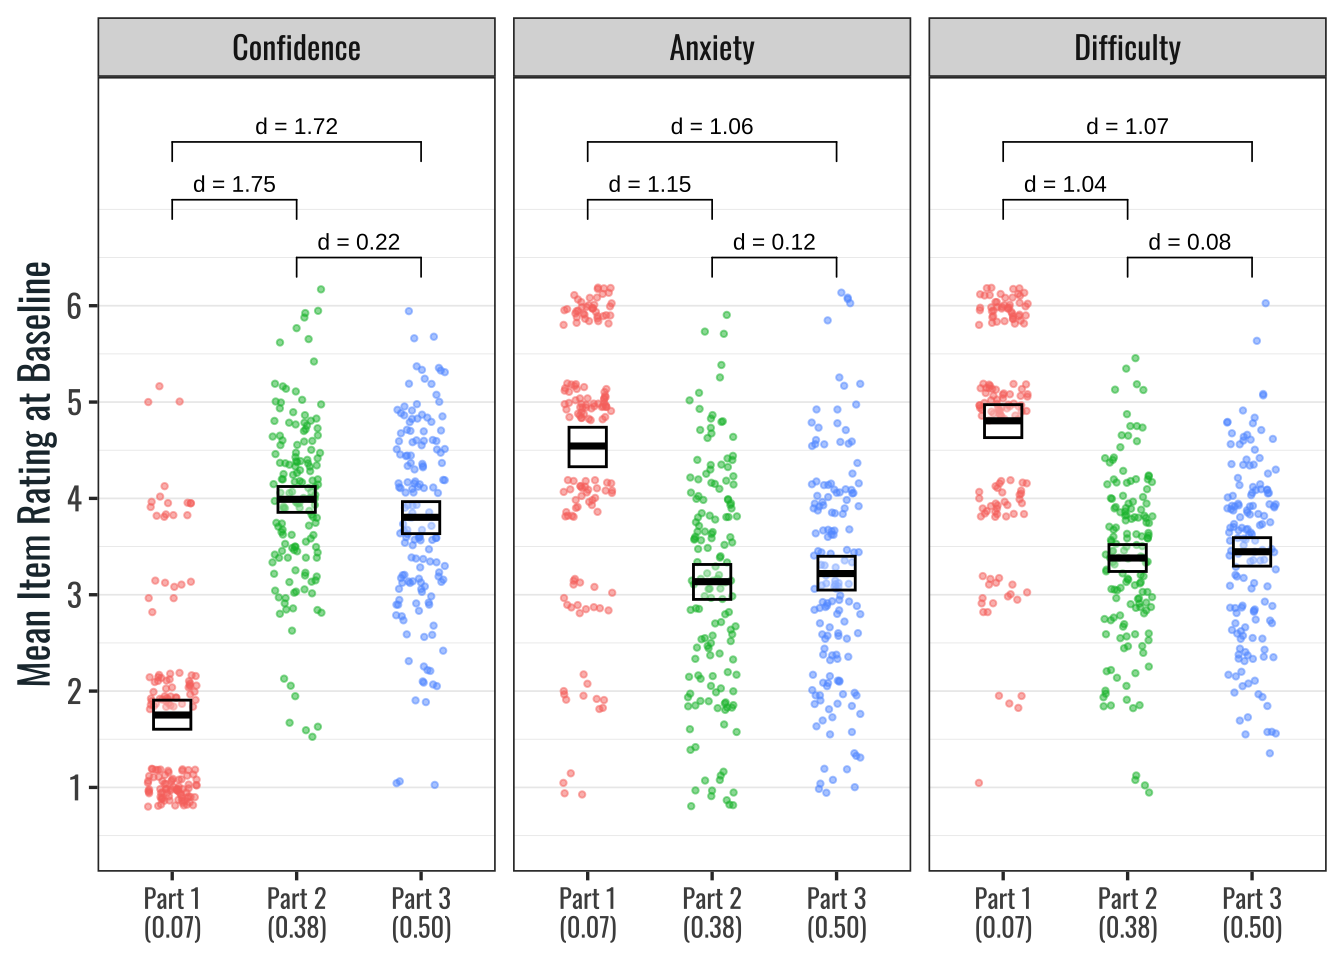
\includegraphics[keepaspectratio]{chapters/07-baseline-correlations_files/figure-pdf/fig-judgment-by-task-1.pdf}}

}

\end{figure}%

\begin{tcolorbox}[enhanced jigsaw, bottomrule=.15mm, breakable, coltitle=black, rightrule=.15mm, colbacktitle=quarto-callout-note-color!10!white, leftrule=.75mm, titlerule=0mm, colframe=quarto-callout-note-color-frame, toprule=.15mm, colback=white, left=2mm, bottomtitle=1mm, opacitybacktitle=0.6, opacityback=0, toptitle=1mm, arc=.35mm, title=\textcolor{quarto-callout-note-color}{\faInfo}\hspace{0.5em}{Note}]

Supplementary Figure~\ref{fig-judgment-by-task}: Cohen's \emph{d} values
for paired samples were obtained by calculating a mean perception rating
for each participant by task and perception type and then dividing the
mean difference by the standard deviation of the difference for each
comparison. Crossbars show means and bootstrapped 95\% confidence
intervals. Mean accuracy for each task is shown in parentheses along the
\emph{x} axis.

\end{tcolorbox}

Perception ratings were sensitive to fluctuations in performance between
the physics tasks, indicating construct validity (see Supplementary
Figure~\ref{fig-judgment-by-task}). For example, there was a large
effect size difference in perceptions of confidence, anxiety, and
difficulty between ratings on the quantitative problem solving item
compared to mean ratings on both the problem categorization items and
the qualitative problem solving items (Cohen's \emph{d} = 1.04 - 1.75).
These differences make sense given that students performed near floor on
the quantitative problem, and considerably better on the other two
tasks. There was a small effect size difference between confidence
ratings on the problem categorization items compared to the qualitative
items (Cohen's \emph{d} = 0.22), with greater confidence reported on the
problem categorization items. A likely explanation is that some of the
categorization items were designed to appear simpler than they are in
reality, so students may have been overconfident on those items. The
difference between anxiety and difficulty ratings on the problem
categorization items compared to the qualitative items was marginal
(Cohen's \emph{d} = 0.12, 0.08). Overall, students' perceptions varied
with mean accuracy on the different types of items.

\chapter{Research Question 1}\label{research-question-1}

\section{Model Specification}\label{model-specification}

Code for model specification not available in PDF format.

\section{Reproduction of Table 4}\label{reproduction-of-table-4}

See Supplementary Table~\ref{tbl-main-tbl-4}

\begin{table}

\caption{\label{tbl-main-tbl-4}Results from Mixed Effects Models Testing
Hypotheses 1-3: Effects of Mindfulness Training on Item-Level Judgments
While Answering Physics Questions}

\centering{

\centering\begingroup\fontsize{8}{10}\selectfont

\resizebox{\ifdim\width>\linewidth\linewidth\else\width\fi}{!}{
\begin{tabular}[t]{>{\raggedright\arraybackslash}p{4cm}>{\raggedright\arraybackslash}p{1cm}>{\raggedright\arraybackslash}p{1cm}>{\raggedright\arraybackslash}p{1cm}>{\raggedright\arraybackslash}p{1cm}>{\raggedright\arraybackslash}p{1cm}>{\raggedright\arraybackslash}p{1cm}>{\raggedright\arraybackslash}p{1cm}>{\raggedright\arraybackslash}p{1cm}>{\raggedright\arraybackslash}p{1cm}}
\toprule
\multicolumn{1}{c}{ } & \multicolumn{3}{c}{H1: Confidence} & \multicolumn{3}{c}{H2: Anxiety} & \multicolumn{3}{c}{H3: Difficulty} \\
\cmidrule(l{3pt}r{3pt}){2-4} \cmidrule(l{3pt}r{3pt}){5-7} \cmidrule(l{3pt}r{3pt}){8-10}
Predictor & Estimate & SE & p & Estimate & SE & p & Estimate & SE & p\\
\midrule
(Intercept) & 3.69 & 0.15 & \textbf{<0.001} & 3.33 & 0.12 & \textbf{<0.001} & 3.56 & 0.12 & \textbf{<0.001}\\
Cohort [Cohort 2] & 0.38 & 0.31 & 0.222 & -0.16 & 0.43 & 0.709 & -0.52 & 0.32 & 0.106\\
Cohort [Cohort 3] & 0.07 & 0.27 & 0.785 & 0.06 & 0.38 & 0.868 & -0.33 & 0.28 & 0.235\\
Semester Week & 0.10 & 0.05 & \textbf{0.036} & -0.04 & 0.07 & 0.537 & -0.12 & 0.05 & \textbf{0.019}\\
Test Version [B] & -0.13 & 0.12 & 0.268 & -0.08 & 0.10 & 0.385 & -0.07 & 0.10 & 0.518\\
\addlinespace
Item-Level Accuracy [Correct] & 0.13 & 0.04 & \textbf{0.005} & -0.08 & 0.04 & \textbf{0.026} & -0.03 & 0.04 & 0.426\\
Baseline Threat & -0.24 & 0.04 & \textbf{<0.001} & 0.22 & 0.06 & \textbf{<0.001} & 0.15 & 0.04 & \textbf{<0.001}\\
Timepoint [Posttest] & 0.19 & 0.04 & \textbf{<0.001} & -0.34 & 0.03 & \textbf{<0.001} & -0.12 & 0.04 & \textbf{<0.001}\\
Condition [Mindfulness] & 0.07 & 0.11 & 0.545 & -0.25 & 0.15 & 0.087 & -0.08 & 0.11 & 0.479\\
Gender [Women or Non-binary] & -0.35 & 0.12 & \textbf{0.003} & 0.49 & 0.16 & \textbf{0.002} & 0.22 & 0.11 & \textbf{0.048}\\
\addlinespace
Timepoint [Posttest] × Condition [Mindfulness] & 0.13 & 0.08 & 0.089 & -0.11 & 0.07 & 0.102 & -0.29 & 0.07 & \textbf{<0.001}\\
Timepoint [Posttest] × Gender [Women or Non-binary] & 0.06 & 0.08 & 0.451 & -0.12 & 0.07 & 0.071 &  &  & \\
Condition [Mindfulness] × Gender [Women or Non-binary] & -0.19 & 0.22 & 0.391 & -0.11 & 0.30 & 0.721 &  &  & \\
(Timepoint [Posttest] × Condition [Mindfulness]) × Gender [Women or Non-binary] & 0.32 & 0.15 & \textbf{0.034} & -0.31 & 0.13 & \textbf{0.018} &  &  & \\
\textbf{Random Effects} & \textbf{} & \textbf{} & \textbf{} & \textbf{} & \textbf{} & \textbf{} & \textbf{} & \textbf{} & \textbf{}\\
\addlinespace
$\sigma^2$ & 1.17 &  &  & 0.87 &  &  & 0.93 &  & \\
$\tau_{00}$ & $0.33_{Participant}$ &  &  & $0.72_{Participant}$ &  &  & $0.37_{Participant}$ &  & \\
 & $0.45_{Item}$ &  &  & $0.17_{Item}$ &  &  & $0.27_{Item}$ &  & \\
ICC & 0.40 &  &  & 0.51 &  &  & 0.41 &  & \\
$N$ & $149_{Participant}$ &  &  & $149_{Participant}$ &  &  & $149_{Participant}$ &  & \\
\addlinespace
 & $22_{Item}$ &  &  & $22_{Item}$ &  &  & $22_{Item}$ &  & \\
Observations & 3275 &  &  & 3275 &  &  & 3275 &  & \\
Marginal $R^2$ / Conditional $R^2$ & 0.099 / 0.461 &  &  & 0.123 / 0.567 &  &  & 0.068 / 0.448 &  & \\
\bottomrule
\end{tabular}}
\endgroup{}

}

\end{table}%

\section{Confidence Judgments: Model
Comparison}\label{confidence-judgments-model-comparison}

See Supplementary Table~\ref{tbl-confidence-models}

\begin{table}

\caption{\label{tbl-confidence-models}Comparison of Models Predicting
Confidence Judgments}

\centering{

\centering\begingroup\fontsize{8}{10}\selectfont

\resizebox{\ifdim\width>\linewidth\linewidth\else\width\fi}{!}{
\begin{tabular}[t]{>{\raggedright\arraybackslash}p{4cm}>{\raggedright\arraybackslash}p{1cm}>{\raggedright\arraybackslash}p{1cm}>{\raggedright\arraybackslash}p{1cm}>{\raggedright\arraybackslash}p{1cm}>{\raggedright\arraybackslash}p{1cm}>{\raggedright\arraybackslash}p{1cm}>{\raggedright\arraybackslash}p{1cm}>{\raggedright\arraybackslash}p{1cm}>{\raggedright\arraybackslash}p{1cm}}
\toprule
\multicolumn{1}{c}{ } & \multicolumn{3}{c}{Accuracy and Baseline Threat Removed} & \multicolumn{3}{c}{2-Way Interaction} & \multicolumn{3}{c}{3-Way Interaction} \\
\cmidrule(l{3pt}r{3pt}){2-4} \cmidrule(l{3pt}r{3pt}){5-7} \cmidrule(l{3pt}r{3pt}){8-10}
Predictor & Estimate & SE & p & Estimate & SE & p & Estimate & SE & p\\
\midrule
(Intercept) & 3.69 & 0.16 & \textbf{<0.001} & 3.69 & 0.15 & \textbf{<0.001} & 3.69 & 0.15 & \textbf{<0.001}\\
Cohort [Cohort 2] & 0.28 & 0.34 & 0.409 & 0.38 & 0.31 & 0.221 & 0.38 & 0.31 & 0.222\\
Cohort [Cohort 3] & 0.01 & 0.30 & 0.977 & 0.07 & 0.27 & 0.786 & 0.07 & 0.27 & 0.785\\
Semester Week & 0.09 & 0.05 & 0.082 & 0.10 & 0.05 & \textbf{0.035} & 0.10 & 0.05 & \textbf{0.036}\\
Test Version [B] & -0.14 & 0.12 & 0.235 & -0.14 & 0.12 & 0.253 & -0.13 & 0.12 & 0.268\\
\addlinespace
Gender [Women or Non-binary] & -0.51 & 0.12 & \textbf{<0.001} & -0.32 & 0.11 & \textbf{0.003} & -0.35 & 0.12 & \textbf{0.003}\\
Timepoint [Posttest] & 0.19 & 0.04 & \textbf{<0.001} & 0.19 & 0.04 & \textbf{<0.001} & 0.19 & 0.04 & \textbf{<0.001}\\
Condition [Mindfulness] & 0.10 & 0.12 & 0.394 & 0.07 & 0.11 & 0.543 & 0.07 & 0.11 & 0.545\\
Timepoint [Posttest] × Condition [Mindfulness] & 0.13 & 0.08 & 0.086 & 0.13 & 0.08 & 0.090 & 0.13 & 0.08 & 0.089\\
Item-Level Accuracy [Correct] &  &  &  & 0.12 & 0.04 & \textbf{0.005} & 0.13 & 0.04 & \textbf{0.005}\\
\addlinespace
Baseline Threat &  &  &  & -0.24 & 0.04 & \textbf{<0.001} & -0.24 & 0.04 & \textbf{<0.001}\\
Timepoint [Posttest] × Gender [Women or Non-binary] &  &  &  &  &  &  & 0.06 & 0.08 & 0.451\\
Condition [Mindfulness] × Gender [Women or Non-binary] &  &  &  &  &  &  & -0.19 & 0.22 & 0.391\\
(Timepoint [Posttest] × Condition [Mindfulness]) × Gender [Women or Non-binary] &  &  &  &  &  &  & 0.32 & 0.15 & \textbf{0.034}\\
\textbf{Random Effects} & \textbf{} & \textbf{} & \textbf{} & \textbf{} & \textbf{} & \textbf{} & \textbf{} & \textbf{} & \textbf{}\\
\addlinespace
$\sigma^2$ & 1.17 &  &  & 1.17 &  &  & 1.17 &  & \\
$\tau_{00}$ & $0.42_{Participant}$ &  &  & $0.33_{Participant}$ &  &  & $0.33_{Participant}$ &  & \\
 & $0.46_{Item}$ &  &  & $0.45_{Item}$ &  &  & $0.45_{Item}$ &  & \\
ICC & 0.43 &  &  & 0.40 &  &  & 0.40 &  & \\
$N$ & $149_{Participant}$ &  &  & $149_{Participant}$ &  &  & $149_{Participant}$ &  & \\
\addlinespace
 & $22_{Item}$ &  &  & $22_{Item}$ &  &  & $22_{Item}$ &  & \\
Observations & 3275 &  &  & 3275 &  &  & 3275 &  & \\
Marginal $R^2$ / Conditional $R^2$ & 0.057 / 0.463 &  &  & 0.099 / 0.460 &  &  & 0.099 / 0.461 &  & \\
\bottomrule
\end{tabular}}
\endgroup{}

}

\end{table}%

\section{Anxiety Judgments: Model
Comparison}\label{anxiety-judgments-model-comparison}

See Supplementary Table~\ref{tbl-anxiety-models}

\begin{table}

\caption{\label{tbl-anxiety-models}Comparison of Models Predicting
Anxiety Judgments}

\centering{

\centering\begingroup\fontsize{8}{10}\selectfont

\resizebox{\ifdim\width>\linewidth\linewidth\else\width\fi}{!}{
\begin{tabular}[t]{>{\raggedright\arraybackslash}p{4cm}>{\raggedright\arraybackslash}p{1cm}>{\raggedright\arraybackslash}p{1cm}>{\raggedright\arraybackslash}p{1cm}>{\raggedright\arraybackslash}p{1cm}>{\raggedright\arraybackslash}p{1cm}>{\raggedright\arraybackslash}p{1cm}>{\raggedright\arraybackslash}p{1cm}>{\raggedright\arraybackslash}p{1cm}>{\raggedright\arraybackslash}p{1cm}}
\toprule
\multicolumn{1}{c}{ } & \multicolumn{3}{c}{Accuracy and Baseline Threat Removed} & \multicolumn{3}{c}{2-Way Interaction} & \multicolumn{3}{c}{3-Way Interaction} \\
\cmidrule(l{3pt}r{3pt}){2-4} \cmidrule(l{3pt}r{3pt}){5-7} \cmidrule(l{3pt}r{3pt}){8-10}
Predictor & Estimate & SE & p & Estimate & SE & p & Estimate & SE & p\\
\midrule
(Intercept) & 3.33 & 0.12 & \textbf{<0.001} & 3.33 & 0.12 & \textbf{<0.001} & 3.33 & 0.12 & \textbf{<0.001}\\
Cohort [Cohort 2] & -0.08 & 0.45 & 0.867 & -0.16 & 0.43 & 0.703 & -0.16 & 0.43 & 0.709\\
Cohort [Cohort 3] & 0.12 & 0.40 & 0.764 & 0.06 & 0.38 & 0.879 & 0.06 & 0.38 & 0.868\\
Semester Week & -0.03 & 0.07 & 0.639 & -0.04 & 0.07 & 0.538 & -0.04 & 0.07 & 0.537\\
Test Version [B] & -0.08 & 0.10 & 0.408 & -0.08 & 0.10 & 0.399 & -0.08 & 0.10 & 0.385\\
\addlinespace
Gender [Women or Non-binary] & 0.60 & 0.16 & \textbf{<0.001} & 0.42 & 0.15 & \textbf{0.006} & 0.49 & 0.16 & \textbf{0.002}\\
Timepoint [Posttest] & -0.34 & 0.03 & \textbf{<0.001} & -0.34 & 0.03 & \textbf{<0.001} & -0.34 & 0.03 & \textbf{<0.001}\\
Condition [Mindfulness] & -0.29 & 0.15 & 0.063 & -0.25 & 0.15 & 0.087 & -0.25 & 0.15 & 0.087\\
Timepoint [Posttest] × Condition [Mindfulness] & -0.11 & 0.07 & 0.102 & -0.11 & 0.07 & 0.105 & -0.11 & 0.07 & 0.102\\
Item-Level Accuracy [Correct] &  &  &  & -0.08 & 0.04 & \textbf{0.028} & -0.08 & 0.04 & \textbf{0.026}\\
\addlinespace
Baseline Threat &  &  &  & 0.23 & 0.06 & \textbf{<0.001} & 0.22 & 0.06 & \textbf{<0.001}\\
Timepoint [Posttest] × Gender [Women or Non-binary] &  &  &  &  &  &  & -0.12 & 0.07 & 0.071\\
Condition [Mindfulness] × Gender [Women or Non-binary] &  &  &  &  &  &  & -0.11 & 0.30 & 0.721\\
(Timepoint [Posttest] × Condition [Mindfulness]) × Gender [Women or Non-binary] &  &  &  &  &  &  & -0.31 & 0.13 & \textbf{0.018}\\
\textbf{Random Effects} & \textbf{} & \textbf{} & \textbf{} & \textbf{} & \textbf{} & \textbf{} & \textbf{} & \textbf{} & \textbf{}\\
\addlinespace
$\sigma^2$ & 0.87 &  &  & 0.87 &  &  & 0.87 &  & \\
$\tau_{00}$ & $0.80_{Participant}$ &  &  & $0.72_{Participant}$ &  &  & $0.72_{Participant}$ &  & \\
 & $0.18_{Item}$ &  &  & $0.17_{Item}$ &  &  & $0.17_{Item}$ &  & \\
ICC & 0.53 &  &  & 0.51 &  &  & 0.51 &  & \\
$N$ & $149_{Participant}$ &  &  & $149_{Participant}$ &  &  & $149_{Participant}$ &  & \\
\addlinespace
 & $22_{Item}$ &  &  & $22_{Item}$ &  &  & $22_{Item}$ &  & \\
Observations & 3275 &  &  & 3275 &  &  & 3275 &  & \\
Marginal $R^2$ / Conditional $R^2$ & 0.078 / 0.565 &  &  & 0.120 / 0.565 &  &  & 0.123 / 0.567 &  & \\
\bottomrule
\end{tabular}}
\endgroup{}

}

\end{table}%

\section{Difficulty Judgments: Model
Comparison}\label{difficulty-judgments-model-comparison}

See Supplementary Table~\ref{tbl-difficulty-models}

\begin{table}

\caption{\label{tbl-difficulty-models}Comparison of Models Predicting
Difficulty Judgments}

\centering{

\centering\begingroup\fontsize{8}{10}\selectfont

\resizebox{\ifdim\width>\linewidth\linewidth\else\width\fi}{!}{
\begin{tabular}[t]{>{\raggedright\arraybackslash}p{4cm}>{\raggedright\arraybackslash}p{1cm}>{\raggedright\arraybackslash}p{1cm}>{\raggedright\arraybackslash}p{1cm}>{\raggedright\arraybackslash}p{1cm}>{\raggedright\arraybackslash}p{1cm}>{\raggedright\arraybackslash}p{1cm}>{\raggedright\arraybackslash}p{1cm}>{\raggedright\arraybackslash}p{1cm}>{\raggedright\arraybackslash}p{1cm}}
\toprule
\multicolumn{1}{c}{ } & \multicolumn{3}{c}{Accuracy and Baseline Threat Removed} & \multicolumn{3}{c}{2-Way Interaction} & \multicolumn{3}{c}{3-Way Interaction} \\
\cmidrule(l{3pt}r{3pt}){2-4} \cmidrule(l{3pt}r{3pt}){5-7} \cmidrule(l{3pt}r{3pt}){8-10}
Predictor & Estimate & SE & p & Estimate & SE & p & Estimate & SE & p\\
\midrule
(Intercept) & 3.56 & 0.13 & \textbf{<0.001} & 3.56 & 0.12 & \textbf{<0.001} & 3.56 & 0.12 & \textbf{<0.001}\\
Cohort [Cohort 2] & -0.46 & 0.33 & 0.166 & -0.52 & 0.32 & 0.106 & -0.52 & 0.32 & 0.107\\
Cohort [Cohort 3] & -0.29 & 0.29 & 0.315 & -0.33 & 0.28 & 0.235 & -0.33 & 0.28 & 0.234\\
Semester Week & -0.11 & 0.05 & \textbf{0.032} & -0.12 & 0.05 & \textbf{0.019} & -0.12 & 0.05 & \textbf{0.019}\\
Test Version [B] & -0.07 & 0.10 & 0.528 & -0.07 & 0.10 & 0.518 & -0.07 & 0.10 & 0.507\\
\addlinespace
Gender [Women or Non-binary] & 0.34 & 0.11 & \textbf{0.003} & 0.22 & 0.11 & \textbf{0.048} & 0.16 & 0.12 & 0.196\\
Timepoint [Posttest] & -0.12 & 0.04 & \textbf{<0.001} & -0.12 & 0.04 & \textbf{<0.001} & -0.12 & 0.04 & \textbf{<0.001}\\
Condition [Mindfulness] & -0.10 & 0.12 & 0.376 & -0.08 & 0.11 & 0.479 & -0.08 & 0.11 & 0.478\\
Timepoint [Posttest] × Condition [Mindfulness] & -0.29 & 0.07 & \textbf{<0.001} & -0.29 & 0.07 & \textbf{<0.001} & -0.29 & 0.07 & \textbf{<0.001}\\
Item-Level Accuracy [Correct] &  &  &  & -0.03 & 0.04 & 0.426 & -0.03 & 0.04 & 0.436\\
\addlinespace
Baseline Threat &  &  &  & 0.15 & 0.04 & \textbf{<0.001} & 0.15 & 0.04 & \textbf{<0.001}\\
Timepoint [Posttest] × Gender [Women or Non-binary] &  &  &  &  &  &  & 0.12 & 0.07 & 0.076\\
Condition [Mindfulness] × Gender [Women or Non-binary] &  &  &  &  &  &  & 0.03 & 0.23 & 0.910\\
(Timepoint [Posttest] × Condition [Mindfulness]) × Gender [Women or Non-binary] &  &  &  &  &  &  & 0.11 & 0.14 & 0.420\\
\textbf{Random Effects} & \textbf{} & \textbf{} & \textbf{} & \textbf{} & \textbf{} & \textbf{} & \textbf{} & \textbf{} & \textbf{}\\
\addlinespace
$\sigma^2$ & 0.93 &  &  & 0.93 &  &  & 0.93 &  & \\
$\tau_{00}$ & $0.41_{Participant}$ &  &  & $0.37_{Participant}$ &  &  & $0.38_{Participant}$ &  & \\
 & $0.27_{Item}$ &  &  & $0.27_{Item}$ &  &  & $0.27_{Item}$ &  & \\
ICC & 0.42 &  &  & 0.41 &  &  & 0.41 &  & \\
$N$ & $149_{Participant}$ &  &  & $149_{Participant}$ &  &  & $149_{Participant}$ &  & \\
\addlinespace
 & $22_{Item}$ &  &  & $22_{Item}$ &  &  & $22_{Item}$ &  & \\
Observations & 3275 &  &  & 3275 &  &  & 3275 &  & \\
Marginal $R^2$ / Conditional $R^2$ & 0.046 / 0.448 &  &  & 0.068 / 0.448 &  &  & 0.068 / 0.449 &  & \\
\bottomrule
\end{tabular}}
\endgroup{}

}

\end{table}%

\section{Reproduction of Figure 4}\label{reproduction-of-figure-4}

See Supplementary Figure~\ref{fig-main-fig-4}

\begin{figure}[!hp]

\caption{\label{fig-main-fig-4}Participants' Mean Judgment Ratings at
Baseline and Posttest by Experimental Condition and Gender}

\centering{

\pandocbounded{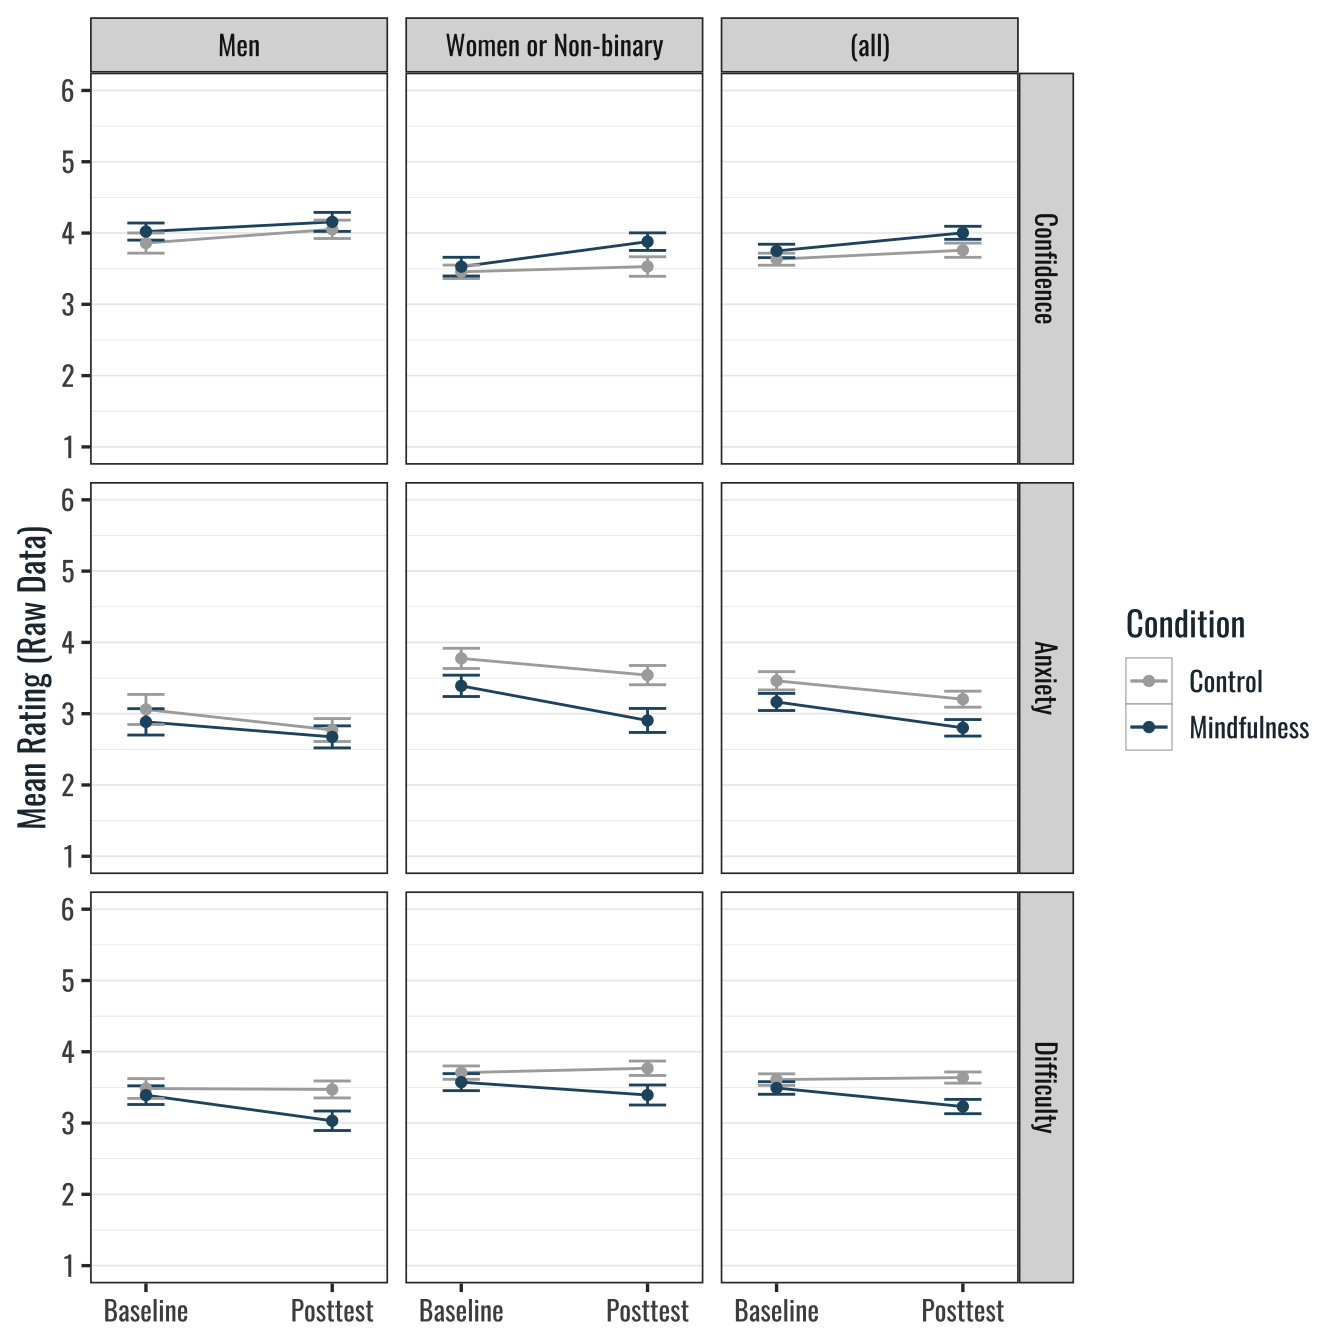
\includegraphics[keepaspectratio]{chapters/08-research-question-1_files/figure-pdf/fig-main-fig-4-1.pdf}}

}

\end{figure}%

\section{Reproduction of Figure 5}\label{reproduction-of-figure-5}

See Supplementary Figure~\ref{fig-main-fig-5}

\begin{figure}[!hp]

\caption{\label{fig-main-fig-5}Estimated Marginal Means for Effects of
Main Variables of Interest}

\centering{

\pandocbounded{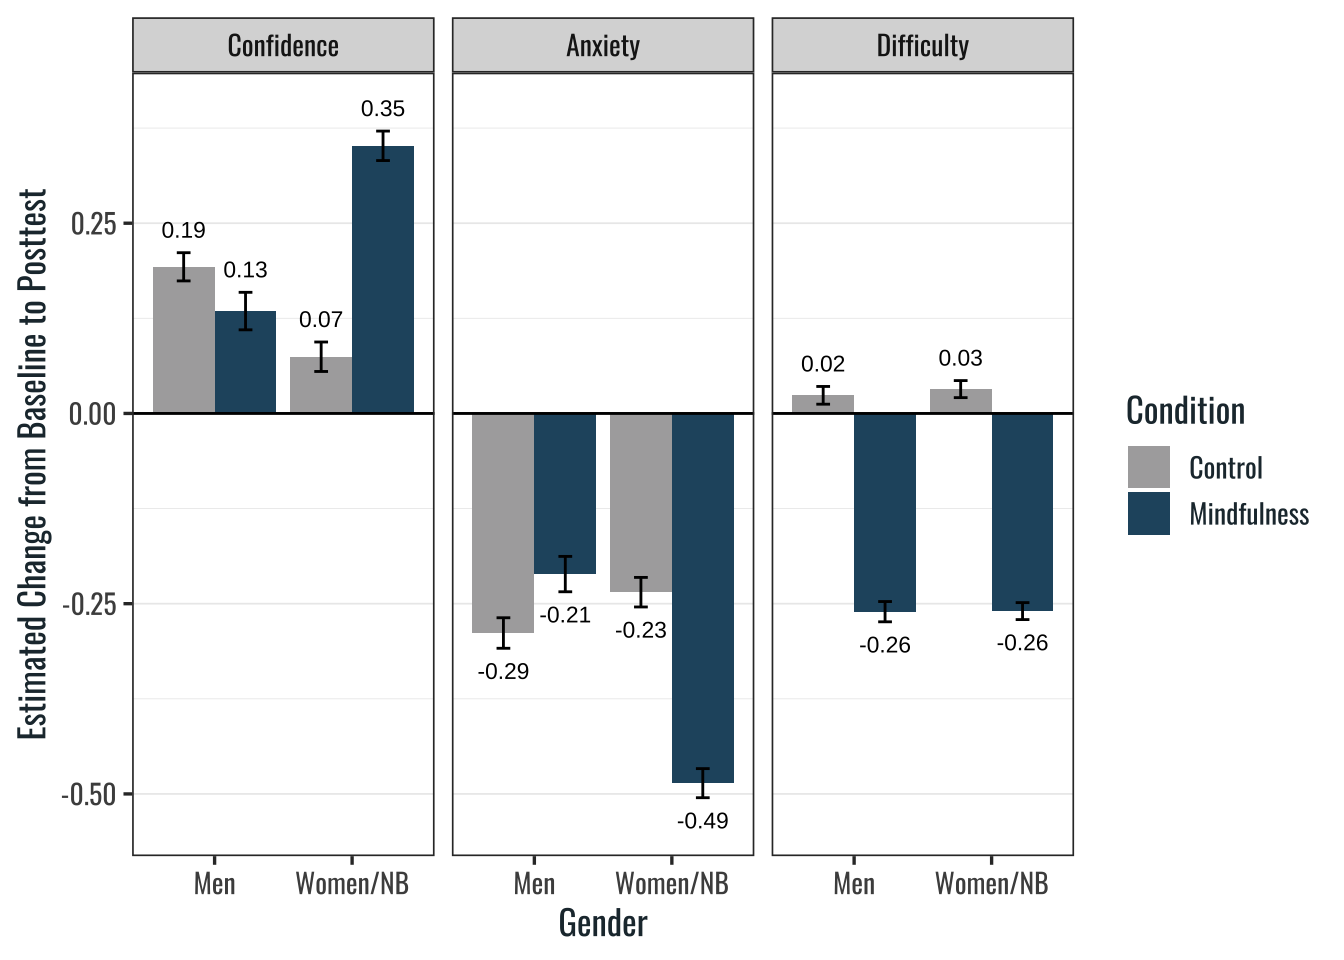
\includegraphics[keepaspectratio]{chapters/08-research-question-1_files/figure-pdf/fig-main-fig-5-1.pdf}}

}

\end{figure}%

\chapter{Research Question 2}\label{research-question-2}

\section{Model Specification}\label{model-specification-1}

Mediation tests were conducted using \texttt{mediation::mediate()} using
bias-corrected bootstrapped confidence intervals.

Code for model specification not available in PDF format.

\section{Confidence}\label{confidence-1}

\subsection{Men Results}\label{men-results}

\subsubsection{Linear Model Results}\label{linear-model-results}

See Supplementary Table~\ref{tbl-conf-men}

\begin{table}

\caption{\label{tbl-conf-men}Mediation Analysis for Confidence at
Posttest: Men}

\centering{

\centering\begingroup\fontsize{8}{10}\selectfont

\resizebox{\ifdim\width>\linewidth\linewidth\else\width\fi}{!}{
\begin{tabular}[t]{>{\raggedright\arraybackslash}p{4cm}>{\raggedright\arraybackslash}p{1cm}>{\raggedright\arraybackslash}p{1cm}>{\raggedright\arraybackslash}p{1cm}>{\raggedright\arraybackslash}p{1cm}>{\raggedright\arraybackslash}p{1cm}>{\raggedright\arraybackslash}p{1cm}>{\raggedright\arraybackslash}p{1cm}>{\raggedright\arraybackslash}p{1cm}>{\raggedright\arraybackslash}p{1cm}}
\toprule
\multicolumn{1}{c}{ } & \multicolumn{3}{c}{Model 1 DV: Posttest Confidence} & \multicolumn{3}{c}{Model 2 DV: EMA Threat} & \multicolumn{3}{c}{Model 3 DV: Posttest Confidence} \\
\cmidrule(l{3pt}r{3pt}){2-4} \cmidrule(l{3pt}r{3pt}){5-7} \cmidrule(l{3pt}r{3pt}){8-10}
Predictor & Estimate & SE & p & Estimate & SE & p & Estimate & SE & p\\
\midrule
(Intercept) & 0.07 & 0.13 & 0.586 & 0.11 & 0.13 & 0.388 & 0.08 & 0.13 & 0.545\\
Condition [Mindfulness] & -0.00 & 0.17 & 0.985 & -0.15 & 0.16 & 0.353 & -0.03 & 0.17 & 0.867\\
Gender [Women or Non-binary] & -0.23 & 0.17 & 0.175 & 0.02 & 0.17 & 0.886 & -0.25 & 0.17 & 0.151\\
Baseline Score & 0.09 & 0.06 & 0.110 & 0.04 & 0.06 & 0.443 & 0.10 & 0.06 & 0.087\\
Cohort 2 & 0.09 & 0.10 & 0.364 & -0.04 & 0.10 & 0.726 & 0.08 & 0.10 & 0.423\\
\addlinespace
Cohort 3 & -0.01 & 0.14 & 0.935 & -0.10 & 0.14 & 0.485 & -0.03 & 0.14 & 0.826\\
Semester Week & 0.03 & 0.15 & 0.838 & -0.02 & 0.14 & 0.895 & 0.01 & 0.15 & 0.919\\
Posttest Test Version [B] & -0.08 & 0.11 & 0.479 & 0.09 & 0.11 & 0.392 & -0.07 & 0.11 & 0.540\\
Baseline Threat & -0.05 & 0.07 & 0.479 & 0.65 & 0.06 & \textbf{<0.001} & 0.05 & 0.09 & 0.594\\
Baseline Confidence & 0.69 & 0.07 & \textbf{<0.001} & -0.17 & 0.07 & \textbf{0.015} & 0.67 & 0.07 & \textbf{<0.001}\\
\addlinespace
Condition [Mindfulness] × Gender [Women or Non-binary] & 0.35 & 0.22 & 0.115 & -0.35 & 0.22 & 0.123 & 0.35 & 0.23 & 0.128\\
EMA Threat &  &  &  &  &  &  & -0.18 & 0.11 & 0.115\\
Gender [Women or Non-binary] × EMA Threat &  &  &  &  &  &  & 0.10 & 0.12 & 0.420\\
Observations & 148 &  &  & 148 &  &  & 148 &  & \\
R2 / R2 adjusted & 0.589 / 0.559 &  &  & 0.590 / 0.561 &  &  & 0.597 / 0.561 &  & \\
\bottomrule
\end{tabular}}
\endgroup{}

}

\end{table}%

\subsubsection{Path Diagram}\label{path-diagram}

See Supplementary Figure~\ref{fig-conf-men}

\begin{figure}[!hp]

\caption{\label{fig-conf-men}Mediation Analysis for Confidence at
Posttest: Men}

\centering{

\pandocbounded{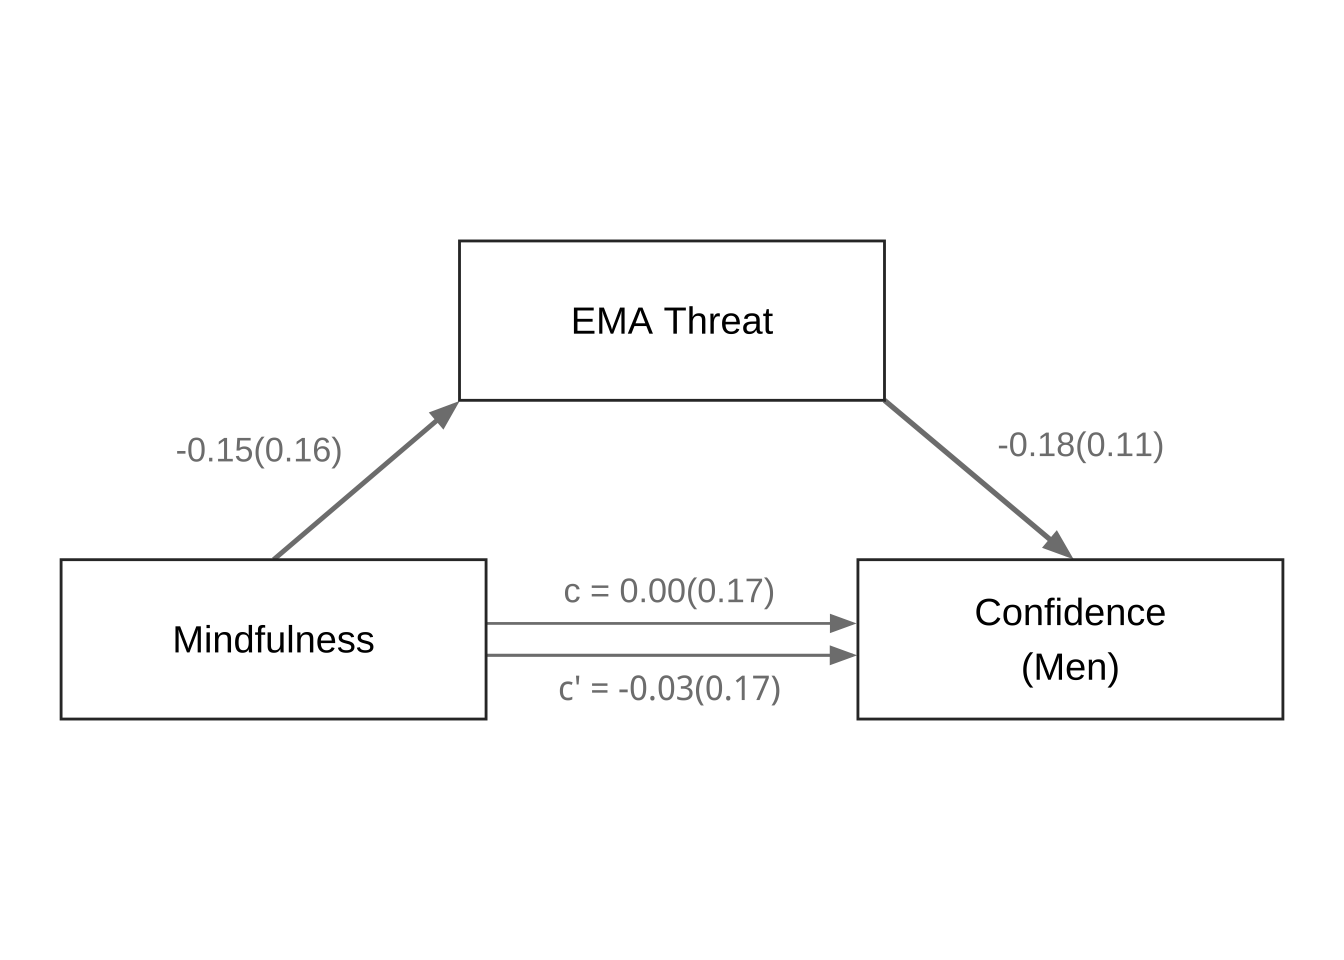
\includegraphics[keepaspectratio]{chapters/09-research-question-2_files/figure-pdf/fig-conf-men-1.pdf}}

}

\end{figure}%

\subsubsection{Mediation Test}\label{mediation-test}

See Supplementary Table~\ref{tbl-med-conf-men}

\begin{table}

\caption{\label{tbl-med-conf-men}Mediation Analysis for Confidence at
Posttest: Men}

\centering{

\centering
\begin{tabular}[t]{lrrrr}
\toprule
Statistic & Estimate & CI Lower & CI Upper & p\\
\midrule
Avg. Causal Mediation Effect & 0.03 & -0.02 & 0.10 & 0.3546\\
Avg. Direct Effect & -0.03 & -0.32 & 0.27 & 0.8776\\
Total Effect & 0.00 & -0.30 & 0.30 & 0.9940\\
Proportion Mediated & -77.28 & -0.29 & 47.14 & 0.8886\\
\bottomrule
\multicolumn{5}{l}{\rule{0pt}{1em}\textit{Note.} Sample Size Used: 148; Simulations: 10000}\\
\end{tabular}

}

\end{table}%

\subsection{Women or Non-binary
Results}\label{women-or-non-binary-results}

\paragraph{Linear Model Results}\label{linear-model-results-1}

See Supplementary Table~\ref{tbl-conf-wnb}

\begin{table}

\caption{\label{tbl-conf-wnb}Mediation Analysis for Confidence at
Posttest: Women}

\centering{

\centering\begingroup\fontsize{8}{10}\selectfont

\resizebox{\ifdim\width>\linewidth\linewidth\else\width\fi}{!}{
\begin{tabular}[t]{>{\raggedright\arraybackslash}p{4cm}>{\raggedright\arraybackslash}p{1cm}>{\raggedright\arraybackslash}p{1cm}>{\raggedright\arraybackslash}p{1cm}>{\raggedright\arraybackslash}p{1cm}>{\raggedright\arraybackslash}p{1cm}>{\raggedright\arraybackslash}p{1cm}>{\raggedright\arraybackslash}p{1cm}>{\raggedright\arraybackslash}p{1cm}>{\raggedright\arraybackslash}p{1cm}}
\toprule
\multicolumn{1}{c}{ } & \multicolumn{3}{c}{Model 1 DV: Posttest Confidence} & \multicolumn{3}{c}{Model 2 DV: EMA Threat} & \multicolumn{3}{c}{Model 3 DV: Posttest Confidence} \\
\cmidrule(l{3pt}r{3pt}){2-4} \cmidrule(l{3pt}r{3pt}){5-7} \cmidrule(l{3pt}r{3pt}){8-10}
Predictor & Estimate & SE & p & Estimate & SE & p & Estimate & SE & p\\
\midrule
(Intercept) & -0.16 & 0.12 & 0.203 & 0.14 & 0.12 & 0.275 & -0.17 & 0.13 & 0.196\\
Condition [Mindfulness] & 0.35 & 0.15 & \textbf{0.019} & -0.50 & 0.15 & \textbf{0.001} & 0.32 & 0.16 & \textbf{0.044}\\
Gender [Men] & 0.23 & 0.17 & 0.175 & -0.02 & 0.17 & 0.886 & 0.25 & 0.17 & 0.151\\
Baseline Score & 0.09 & 0.06 & 0.110 & 0.04 & 0.06 & 0.443 & 0.10 & 0.06 & 0.087\\
Cohort 2 & 0.09 & 0.10 & 0.364 & -0.04 & 0.10 & 0.726 & 0.08 & 0.10 & 0.423\\
\addlinespace
Cohort 3 & -0.01 & 0.14 & 0.935 & -0.10 & 0.14 & 0.485 & -0.03 & 0.14 & 0.826\\
Semester Week & 0.03 & 0.15 & 0.838 & -0.02 & 0.14 & 0.895 & 0.01 & 0.15 & 0.919\\
Posttest Test Version [B] & -0.08 & 0.11 & 0.479 & 0.09 & 0.11 & 0.392 & -0.07 & 0.11 & 0.540\\
Baseline Threat & -0.05 & 0.07 & 0.479 & 0.65 & 0.06 & \textbf{<0.001} & 0.05 & 0.09 & 0.594\\
Baseline Confidence & 0.69 & 0.07 & \textbf{<0.001} & -0.17 & 0.07 & \textbf{0.015} & 0.67 & 0.07 & \textbf{<0.001}\\
\addlinespace
Condition [Mindfulness] × Gender [Men] & -0.35 & 0.22 & 0.115 & 0.35 & 0.22 & 0.123 & -0.35 & 0.23 & 0.128\\
EMA Threat &  &  &  &  &  &  & -0.08 & 0.10 & 0.401\\
Gender [Men] × EMA Threat &  &  &  &  &  &  & -0.10 & 0.12 & 0.420\\
Observations & 148 &  &  & 148 &  &  & 148 &  & \\
R2 / R2 adjusted & 0.589 / 0.559 &  &  & 0.590 / 0.561 &  &  & 0.597 / 0.561 &  & \\
\bottomrule
\end{tabular}}
\endgroup{}

}

\end{table}%

\paragraph{Path Diagram}\label{path-diagram-1}

See Supplementary Figure~\ref{fig-conf-wnb}

\begin{figure}[!hp]

\caption{\label{fig-conf-wnb}Mediation Analysis for Confidence at
Posttest: Women}

\centering{

\pandocbounded{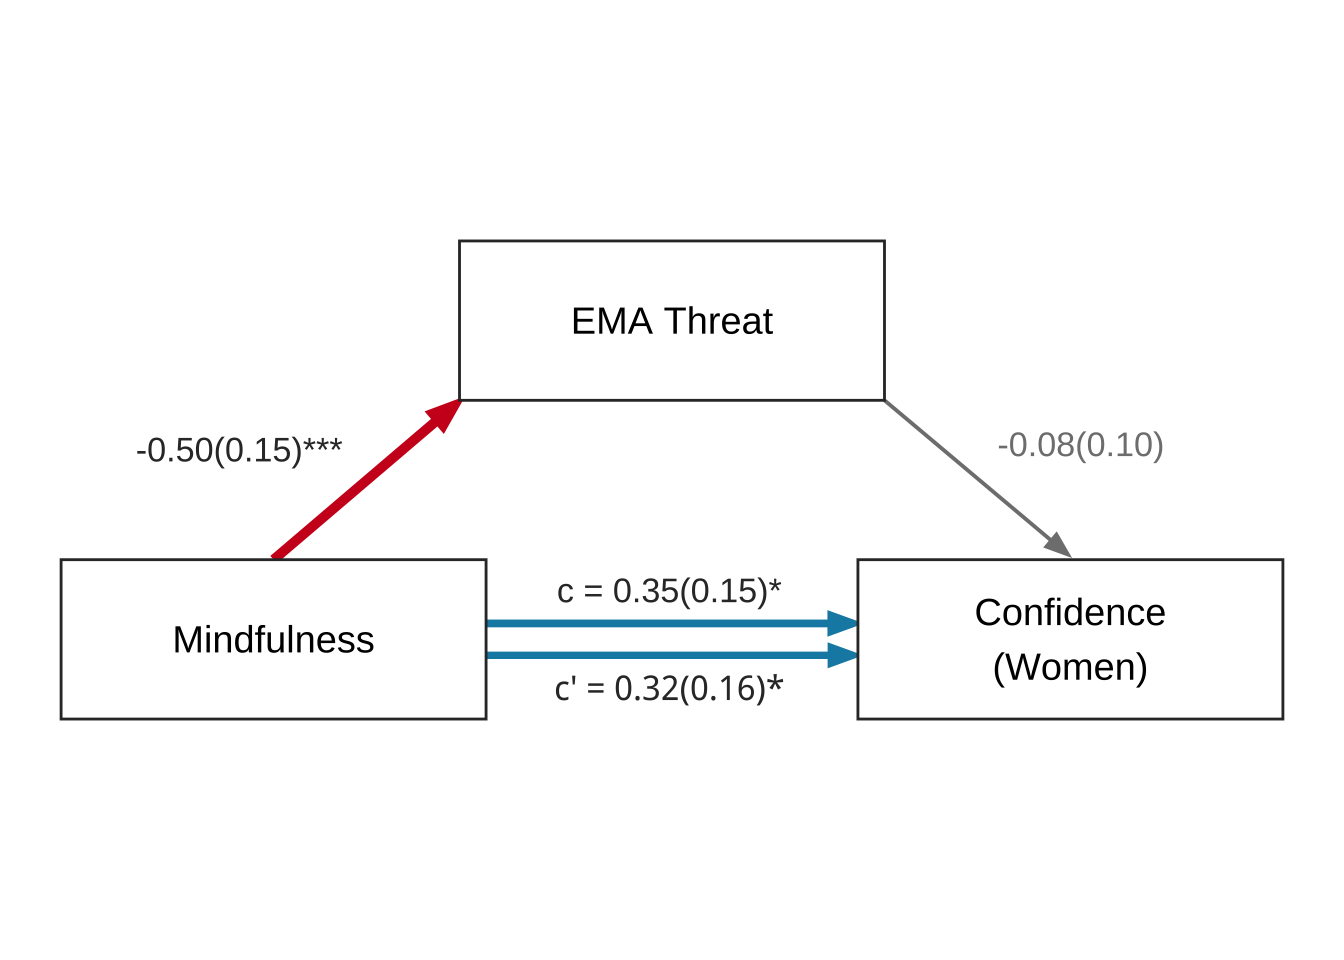
\includegraphics[keepaspectratio]{chapters/09-research-question-2_files/figure-pdf/fig-conf-wnb-1.pdf}}

}

\end{figure}%

\paragraph{Mediation Test}\label{mediation-test-1}

See Supplementary Table~\ref{tbl-med-conf-wnb}

\begin{table}

\caption{\label{tbl-med-conf-wnb}Mediation Analysis for Confidence at
Posttest: Women}

\centering{

\centering
\begin{tabular}[t]{lrrrr}
\toprule
Statistic & Estimate & CI Lower & CI Upper & p\\
\midrule
Avg. Causal Mediation Effect & 0.04 & -0.03 & 0.19 & 0.3432\\
Avg. Direct Effect & 0.32 & 0.01 & 0.63 & 0.0444\\
Total Effect & 0.36 & 0.07 & 0.67 & 0.0140\\
Proportion Mediated & 0.11 & -0.03 & 3.84 & 0.3500\\
\bottomrule
\multicolumn{5}{l}{\rule{0pt}{1em}\textit{Note.} Sample Size Used: 148; Simulations: 10000}\\
\end{tabular}

}

\end{table}%

\section{Anxiety}\label{anxiety-1}

\subsection{Men Results}\label{men-results-1}

\subsubsection{Linear Model Results}\label{linear-model-results-2}

See Supplementary Table~\ref{tbl-anx-men}

\begin{table}

\caption{\label{tbl-anx-men}Mediation Analysis for Anxiety at Posttest:
Men}

\centering{

\centering\begingroup\fontsize{8}{10}\selectfont

\resizebox{\ifdim\width>\linewidth\linewidth\else\width\fi}{!}{
\begin{tabular}[t]{>{\raggedright\arraybackslash}p{4cm}>{\raggedright\arraybackslash}p{1cm}>{\raggedright\arraybackslash}p{1cm}>{\raggedright\arraybackslash}p{1cm}>{\raggedright\arraybackslash}p{1cm}>{\raggedright\arraybackslash}p{1cm}>{\raggedright\arraybackslash}p{1cm}>{\raggedright\arraybackslash}p{1cm}>{\raggedright\arraybackslash}p{1cm}>{\raggedright\arraybackslash}p{1cm}}
\toprule
\multicolumn{1}{c}{ } & \multicolumn{3}{c}{Model 1 DV: Posttest Anxiety} & \multicolumn{3}{c}{Model 2 DV: EMA Threat} & \multicolumn{3}{c}{Model 3 DV: Posttest Anxiety} \\
\cmidrule(l{3pt}r{3pt}){2-4} \cmidrule(l{3pt}r{3pt}){5-7} \cmidrule(l{3pt}r{3pt}){8-10}
Predictor & Estimate & SE & p & Estimate & SE & p & Estimate & SE & p\\
\midrule
(Intercept) & -0.08 & 0.13 & 0.551 & 0.12 & 0.13 & 0.337 & -0.11 & 0.13 & 0.392\\
Condition [Mindfulness] & 0.00 & 0.16 & 0.991 & -0.16 & 0.16 & 0.334 & 0.03 & 0.16 & 0.872\\
Gender [Women or Non-binary] & 0.24 & 0.17 & 0.155 & -0.01 & 0.17 & 0.935 & 0.22 & 0.17 & 0.193\\
Baseline Score & -0.08 & 0.06 & 0.169 & 0.03 & 0.06 & 0.624 & -0.08 & 0.06 & 0.145\\
Cohort 2 & -0.03 & 0.10 & 0.751 & -0.05 & 0.10 & 0.631 & -0.03 & 0.10 & 0.756\\
\addlinespace
Cohort 3 & -0.04 & 0.14 & 0.773 & -0.12 & 0.14 & 0.390 & -0.03 & 0.14 & 0.849\\
Semester Week & -0.10 & 0.14 & 0.465 & -0.07 & 0.14 & 0.611 & -0.11 & 0.14 & 0.455\\
Posttest Test Version [B] & 0.09 & 0.11 & 0.439 & 0.09 & 0.11 & 0.427 & 0.07 & 0.11 & 0.538\\
Baseline Threat & 0.07 & 0.06 & 0.263 & 0.67 & 0.06 & \textbf{<0.001} & -0.05 & 0.08 & 0.558\\
Baseline Anxiety & 0.68 & 0.06 & \textbf{<0.001} & 0.18 & 0.06 & \textbf{0.004} & 0.65 & 0.06 & \textbf{<0.001}\\
\addlinespace
Condition [Mindfulness] × Gender [Women or Non-binary] & -0.37 & 0.22 & 0.100 & -0.29 & 0.22 & 0.190 & -0.26 & 0.22 & 0.254\\
EMA Threat &  &  &  &  &  &  & 0.12 & 0.11 & 0.268\\
Gender [Women or Non-binary] × EMA Threat &  &  &  &  &  &  & 0.13 & 0.12 & 0.261\\
Observations & 148 &  &  & 148 &  &  & 148 &  & \\
R2 / R2 adjusted & 0.589 / 0.559 &  &  & 0.597 / 0.568 &  &  & 0.610 / 0.575 &  & \\
\bottomrule
\end{tabular}}
\endgroup{}

}

\end{table}%

\subsubsection{Path Diagram}\label{path-diagram-2}

See Supplementary Figure~\ref{fig-anx-men}

\begin{figure}[!hp]

\caption{\label{fig-anx-men}Mediation Analysis for Anxiety at Posttest:
Men}

\centering{

\pandocbounded{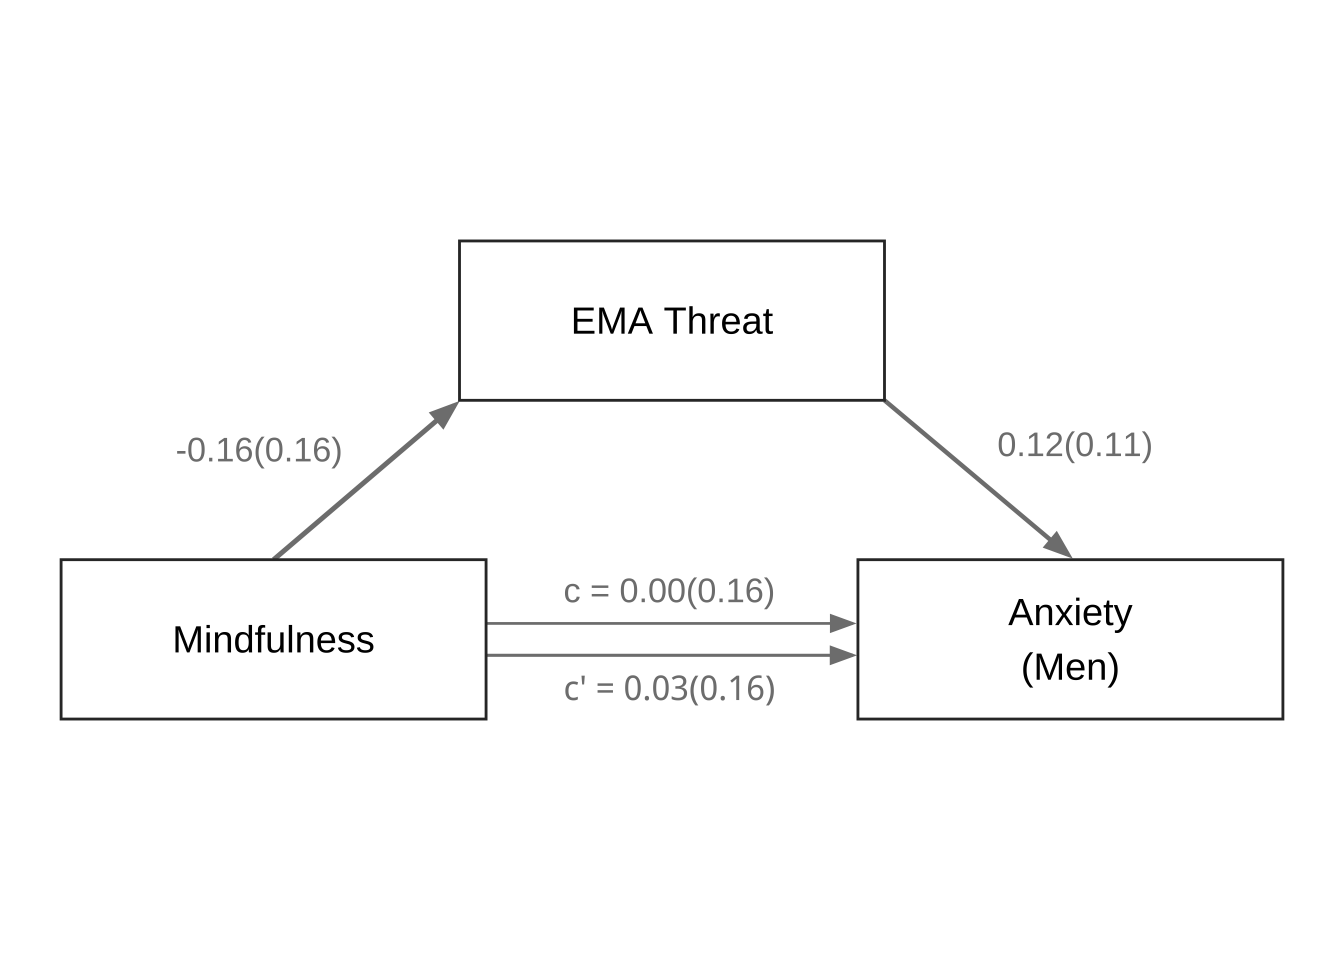
\includegraphics[keepaspectratio]{chapters/09-research-question-2_files/figure-pdf/fig-anx-men-1.pdf}}

}

\end{figure}%

\subsubsection{Mediation Test}\label{mediation-test-2}

See Supplementary Table~\ref{tbl-med-anx-men}

\begin{table}

\caption{\label{tbl-med-anx-men}Mediation Analysis for Anxiety at
Posttest: Men}

\centering{

\centering
\begin{tabular}[t]{lrrrr}
\toprule
Statistic & Estimate & CI Lower & CI Upper & p\\
\midrule
Avg. Causal Mediation Effect & -0.02 & -0.13 & 0.01 & 0.4680\\
Avg. Direct Effect & 0.03 & -0.29 & 0.33 & 0.8690\\
Total Effect & 0.01 & -0.31 & 0.31 & 0.9702\\
Proportion Mediated & -2.98 & 0.09 & 2292.06 & 0.9298\\
\bottomrule
\multicolumn{5}{l}{\rule{0pt}{1em}\textit{Note.} Sample Size Used: 148; Simulations: 10000}\\
\end{tabular}

}

\end{table}%

\subsection{Women or Non-binary
Results}\label{women-or-non-binary-results-1}

\paragraph{Linear Model Results}\label{linear-model-results-3}

See Supplementary Table~\ref{tbl-anx-wnb}

\begin{table}

\caption{\label{tbl-anx-wnb}Mediation Analysis for Anxiety at Posttest:
Women}

\centering{

\centering\begingroup\fontsize{8}{10}\selectfont

\resizebox{\ifdim\width>\linewidth\linewidth\else\width\fi}{!}{
\begin{tabular}[t]{>{\raggedright\arraybackslash}p{4cm}>{\raggedright\arraybackslash}p{1cm}>{\raggedright\arraybackslash}p{1cm}>{\raggedright\arraybackslash}p{1cm}>{\raggedright\arraybackslash}p{1cm}>{\raggedright\arraybackslash}p{1cm}>{\raggedright\arraybackslash}p{1cm}>{\raggedright\arraybackslash}p{1cm}>{\raggedright\arraybackslash}p{1cm}>{\raggedright\arraybackslash}p{1cm}}
\toprule
\multicolumn{1}{c}{ } & \multicolumn{3}{c}{Model 1 DV: Posttest Anxiety} & \multicolumn{3}{c}{Model 2 DV: EMA Threat} & \multicolumn{3}{c}{Model 3 DV: Posttest Anxiety} \\
\cmidrule(l{3pt}r{3pt}){2-4} \cmidrule(l{3pt}r{3pt}){5-7} \cmidrule(l{3pt}r{3pt}){8-10}
Predictor & Estimate & SE & p & Estimate & SE & p & Estimate & SE & p\\
\midrule
(Intercept) & 0.17 & 0.13 & 0.188 & 0.11 & 0.12 & 0.377 & 0.11 & 0.13 & 0.384\\
Condition [Mindfulness] & -0.37 & 0.15 & \textbf{0.015} & -0.45 & 0.15 & \textbf{0.003} & -0.23 & 0.16 & 0.140\\
Gender [Men] & -0.24 & 0.17 & 0.155 & 0.01 & 0.17 & 0.935 & -0.22 & 0.17 & 0.193\\
Baseline Score & -0.08 & 0.06 & 0.169 & 0.03 & 0.06 & 0.624 & -0.08 & 0.06 & 0.145\\
Cohort 2 & -0.03 & 0.10 & 0.751 & -0.05 & 0.10 & 0.631 & -0.03 & 0.10 & 0.756\\
\addlinespace
Cohort 3 & -0.04 & 0.14 & 0.773 & -0.12 & 0.14 & 0.390 & -0.03 & 0.14 & 0.849\\
Semester Week & -0.10 & 0.14 & 0.465 & -0.07 & 0.14 & 0.611 & -0.11 & 0.14 & 0.455\\
Posttest Test Version [B] & 0.09 & 0.11 & 0.439 & 0.09 & 0.11 & 0.427 & 0.07 & 0.11 & 0.538\\
Baseline Threat & 0.07 & 0.06 & 0.263 & 0.67 & 0.06 & \textbf{<0.001} & -0.05 & 0.08 & 0.558\\
Baseline Anxiety & 0.68 & 0.06 & \textbf{<0.001} & 0.18 & 0.06 & \textbf{0.004} & 0.65 & 0.06 & \textbf{<0.001}\\
\addlinespace
Condition [Mindfulness] × Gender [Men] & 0.37 & 0.22 & 0.100 & 0.29 & 0.22 & 0.190 & 0.26 & 0.22 & 0.254\\
EMA Threat &  &  &  &  &  &  & 0.26 & 0.10 & \textbf{0.009}\\
Gender [Men] × EMA Threat &  &  &  &  &  &  & -0.13 & 0.12 & 0.261\\
Observations & 148 &  &  & 148 &  &  & 148 &  & \\
R2 / R2 adjusted & 0.589 / 0.559 &  &  & 0.597 / 0.568 &  &  & 0.610 / 0.575 &  & \\
\bottomrule
\end{tabular}}
\endgroup{}

}

\end{table}%

\paragraph{Path Diagram}\label{path-diagram-3}

See Supplementary Figure~\ref{fig-anx-wnb}

\begin{figure}[!hp]

\caption{\label{fig-anx-wnb}Mediation Analysis for Confidence at
Posttest: Women}

\centering{

\pandocbounded{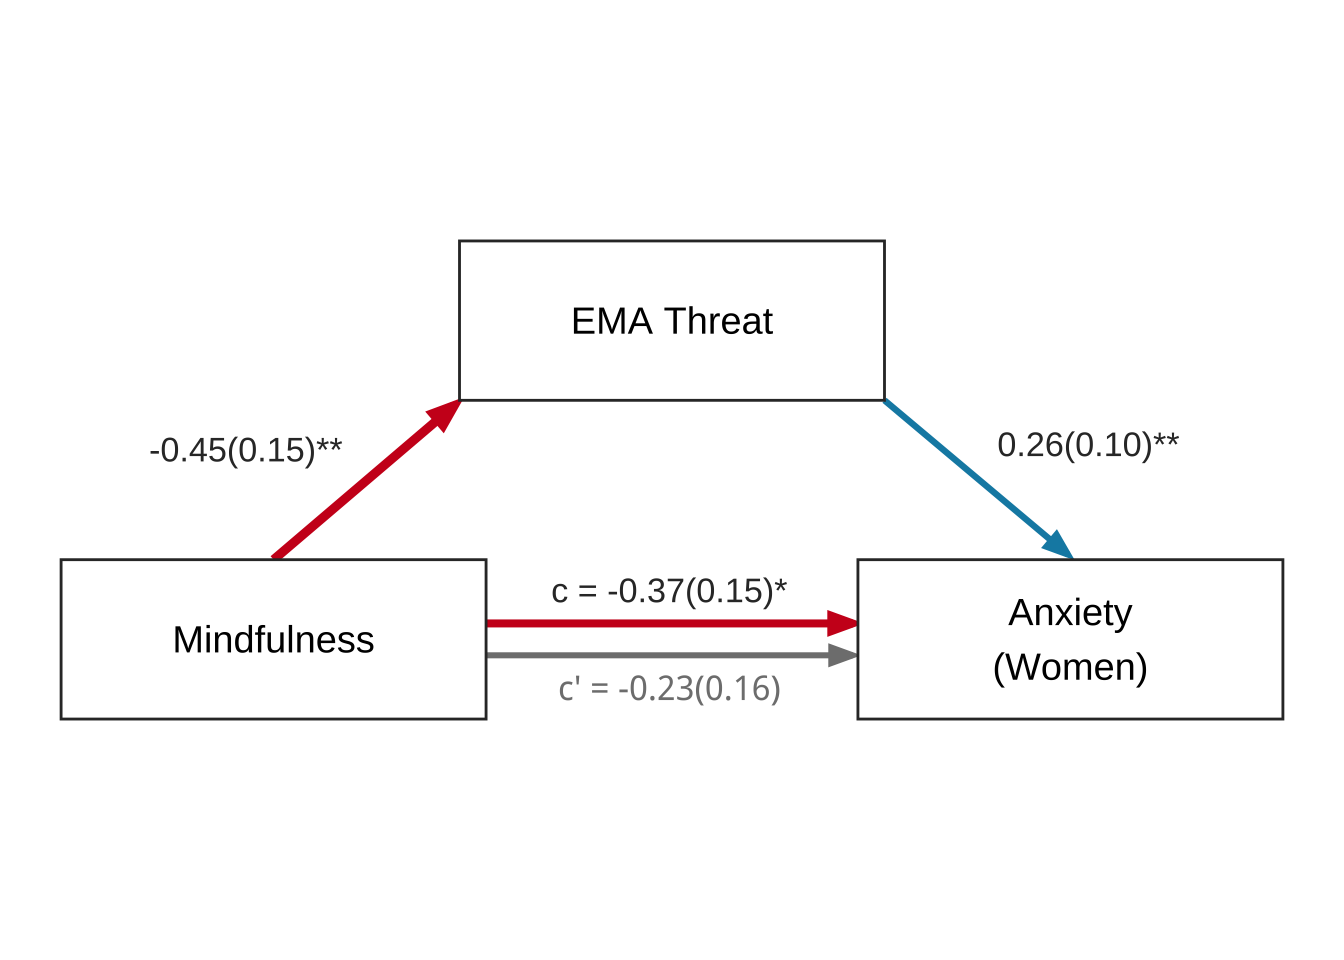
\includegraphics[keepaspectratio]{chapters/09-research-question-2_files/figure-pdf/fig-anx-wnb-1.pdf}}

}

\end{figure}%

\paragraph{Mediation Test}\label{mediation-test-3}

See Supplementary Table~\ref{tbl-med-anx-wnb}

\begin{table}

\caption{\label{tbl-med-anx-wnb}Mediation Analysis for Confidence at
Posttest: Women}

\centering{

\centering
\begin{tabular}[t]{lrrrr}
\toprule
Statistic & Estimate & CI Lower & CI Upper & p\\
\midrule
Avg. Causal Mediation Effect & -0.11 & -0.32 & -0.02 & 0.0176\\
Avg. Direct Effect & -0.23 & -0.55 & 0.11 & 0.1858\\
Total Effect & -0.35 & -0.66 & -0.04 & 0.0284\\
Proportion Mediated & 0.33 & 0.02 & 2.11 & 0.0436\\
\bottomrule
\multicolumn{5}{l}{\rule{0pt}{1em}\textit{Note.} Sample Size Used: 148; Simulations: 10000}\\
\end{tabular}

}

\end{table}%

\section{Difficulty}\label{difficulty-1}

\subsection{Men Results}\label{men-results-2}

\subsubsection{Linear Model Results}\label{linear-model-results-4}

See Supplementary Table~\ref{tbl-diff-men}

\begin{table}

\caption{\label{tbl-diff-men}Mediation Analysis for Difficulty at
Posttest: Men}

\centering{

\centering\begingroup\fontsize{8}{10}\selectfont

\resizebox{\ifdim\width>\linewidth\linewidth\else\width\fi}{!}{
\begin{tabular}[t]{>{\raggedright\arraybackslash}p{4cm}>{\raggedright\arraybackslash}p{1cm}>{\raggedright\arraybackslash}p{1cm}>{\raggedright\arraybackslash}p{1cm}>{\raggedright\arraybackslash}p{1cm}>{\raggedright\arraybackslash}p{1cm}>{\raggedright\arraybackslash}p{1cm}>{\raggedright\arraybackslash}p{1cm}>{\raggedright\arraybackslash}p{1cm}>{\raggedright\arraybackslash}p{1cm}}
\toprule
\multicolumn{1}{c}{ } & \multicolumn{3}{c}{Model 1 DV: Posttest Difficulty} & \multicolumn{3}{c}{Model 2 DV: EMA Threat} & \multicolumn{3}{c}{Model 3 DV: Posttest Difficulty} \\
\cmidrule(l{3pt}r{3pt}){2-4} \cmidrule(l{3pt}r{3pt}){5-7} \cmidrule(l{3pt}r{3pt}){8-10}
Predictor & Estimate & SE & p & Estimate & SE & p & Estimate & SE & p\\
\midrule
(Intercept) & 0.09 & 0.14 & 0.519 & 0.10 & 0.13 & 0.440 & 0.09 & 0.14 & 0.516\\
Condition [Mindfulness] & -0.47 & 0.18 & \textbf{0.009} & -0.17 & 0.16 & 0.298 & -0.47 & 0.18 & \textbf{0.009}\\
Gender [Women or Non-binary] & 0.16 & 0.18 & 0.377 & 0.05 & 0.17 & 0.763 & 0.16 & 0.18 & 0.380\\
Baseline Score & -0.04 & 0.06 & 0.465 & 0.04 & 0.06 & 0.496 & -0.04 & 0.06 & 0.474\\
Cohort 2 & -0.15 & 0.11 & 0.166 & -0.03 & 0.10 & 0.747 & -0.15 & 0.11 & 0.170\\
\addlinespace
Cohort 3 & -0.18 & 0.15 & 0.243 & -0.09 & 0.14 & 0.527 & -0.18 & 0.16 & 0.246\\
Semester Week & -0.12 & 0.15 & 0.446 & -0.02 & 0.15 & 0.880 & -0.12 & 0.16 & 0.454\\
Posttest Test Version [B] & 0.05 & 0.12 & 0.669 & 0.09 & 0.11 & 0.426 & 0.05 & 0.12 & 0.664\\
Baseline Threat & -0.01 & 0.07 & 0.891 & 0.68 & 0.06 & \textbf{<0.001} & 0.00 & 0.09 & 0.995\\
Baseline Difficulty & 0.66 & 0.07 & \textbf{<0.001} & 0.15 & 0.06 & \textbf{0.018} & 0.67 & 0.07 & \textbf{<0.001}\\
\addlinespace
Condition [Mindfulness] × Gender [Women or Non-binary] & 0.12 & 0.24 & 0.609 & -0.31 & 0.22 & 0.165 & 0.12 & 0.25 & 0.639\\
EMA Threat &  &  &  &  &  &  & -0.01 & 0.12 & 0.916\\
Gender [Women or Non-binary] × EMA Threat &  &  &  &  &  &  & -0.00 & 0.13 & 0.976\\
Observations & 148 &  &  & 148 &  &  & 148 &  & \\
R2 / R2 adjusted & 0.535 / 0.501 &  &  & 0.590 / 0.560 &  &  & 0.535 / 0.493 &  & \\
\bottomrule
\end{tabular}}
\endgroup{}

}

\end{table}%

\subsubsection{Path Diagram}\label{path-diagram-4}

See Supplementary Figure~\ref{fig-diff-men}

\begin{figure}[!hp]

\caption{\label{fig-diff-men}Mediation Analysis for Difficulty at
Posttest: Men}

\centering{

\pandocbounded{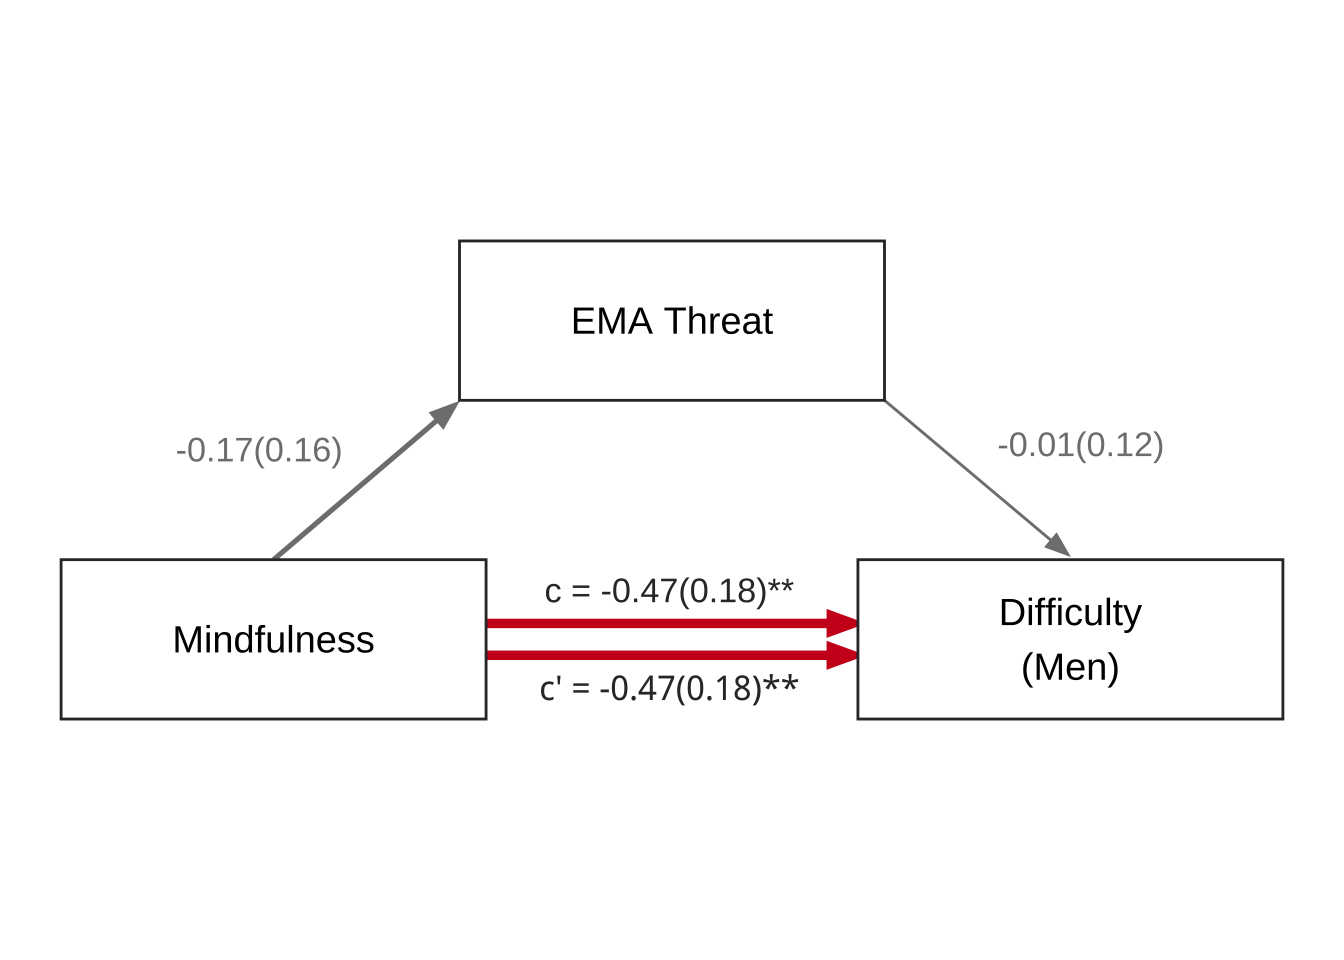
\includegraphics[keepaspectratio]{chapters/09-research-question-2_files/figure-pdf/fig-diff-men-1.pdf}}

}

\end{figure}%

\subsubsection{Mediation Test}\label{mediation-test-4}

See Supplementary Table~\ref{tbl-med-diff-men}

\begin{table}

\caption{\label{tbl-med-diff-men}Mediation Analysis for Difficulty at
Posttest: Men}

\centering{

\centering
\begin{tabular}[t]{lrrrr}
\toprule
Statistic & Estimate & CI Lower & CI Upper & p\\
\midrule
Avg. Causal Mediation Effect & 0.00 & -0.03 & 0.09 & 0.8944\\
Avg. Direct Effect & -0.47 & -0.80 & -0.13 & 0.0070\\
Total Effect & -0.47 & -0.79 & -0.13 & 0.0064\\
Proportion Mediated & 0.00 & -0.31 & 0.06 & 0.8940\\
\bottomrule
\multicolumn{5}{l}{\rule{0pt}{1em}\textit{Note.} Sample Size Used: 148; Simulations: 10000}\\
\end{tabular}

}

\end{table}%

\subsection{Women or Non-binary
Results}\label{women-or-non-binary-results-2}

\subsubsection{Linear Model Results}\label{linear-model-results-5}

See Supplementary Table~\ref{tbl-diff-wnb}

\begin{table}

\caption{\label{tbl-diff-wnb}Mediation Analysis for Difficulty at
Posttest: Women}

\centering{

\centering\begingroup\fontsize{8}{10}\selectfont

\resizebox{\ifdim\width>\linewidth\linewidth\else\width\fi}{!}{
\begin{tabular}[t]{>{\raggedright\arraybackslash}p{4cm}>{\raggedright\arraybackslash}p{1cm}>{\raggedright\arraybackslash}p{1cm}>{\raggedright\arraybackslash}p{1cm}>{\raggedright\arraybackslash}p{1cm}>{\raggedright\arraybackslash}p{1cm}>{\raggedright\arraybackslash}p{1cm}>{\raggedright\arraybackslash}p{1cm}>{\raggedright\arraybackslash}p{1cm}>{\raggedright\arraybackslash}p{1cm}}
\toprule
\multicolumn{1}{c}{ } & \multicolumn{3}{c}{Model 1 DV: Posttest Difficulty} & \multicolumn{3}{c}{Model 2 DV: EMA Threat} & \multicolumn{3}{c}{Model 3 DV: Posttest Difficulty} \\
\cmidrule(l{3pt}r{3pt}){2-4} \cmidrule(l{3pt}r{3pt}){5-7} \cmidrule(l{3pt}r{3pt}){8-10}
Predictor & Estimate & SE & p & Estimate & SE & p & Estimate & SE & p\\
\midrule
(Intercept) & 0.25 & 0.13 & 0.063 & 0.15 & 0.12 & 0.225 & 0.25 & 0.14 & 0.070\\
Condition [Mindfulness] & -0.34 & 0.16 & \textbf{0.031} & -0.48 & 0.15 & \textbf{0.001} & -0.35 & 0.17 & \textbf{0.040}\\
Gender [Men] & -0.16 & 0.18 & 0.377 & -0.05 & 0.17 & 0.763 & -0.16 & 0.18 & 0.380\\
Baseline Score & -0.04 & 0.06 & 0.465 & 0.04 & 0.06 & 0.496 & -0.04 & 0.06 & 0.474\\
Cohort 2 & -0.15 & 0.11 & 0.166 & -0.03 & 0.10 & 0.747 & -0.15 & 0.11 & 0.170\\
\addlinespace
Cohort 3 & -0.18 & 0.15 & 0.243 & -0.09 & 0.14 & 0.527 & -0.18 & 0.16 & 0.246\\
Semester Week & -0.12 & 0.15 & 0.446 & -0.02 & 0.15 & 0.880 & -0.12 & 0.16 & 0.454\\
Posttest Test Version [B] & 0.05 & 0.12 & 0.669 & 0.09 & 0.11 & 0.426 & 0.05 & 0.12 & 0.664\\
Baseline Threat & -0.01 & 0.07 & 0.891 & 0.68 & 0.06 & \textbf{<0.001} & 0.00 & 0.09 & 0.995\\
Baseline Difficulty & 0.66 & 0.07 & \textbf{<0.001} & 0.15 & 0.06 & \textbf{0.018} & 0.67 & 0.07 & \textbf{<0.001}\\
\addlinespace
Condition [Mindfulness] × Gender [Men] & -0.12 & 0.24 & 0.609 & 0.31 & 0.22 & 0.165 & -0.12 & 0.25 & 0.639\\
EMA Threat &  &  &  &  &  &  & -0.02 & 0.10 & 0.875\\
Gender [Men] × EMA Threat &  &  &  &  &  &  & 0.00 & 0.13 & 0.976\\
Observations & 148 &  &  & 148 &  &  & 148 &  & \\
R2 / R2 adjusted & 0.535 / 0.501 &  &  & 0.590 / 0.560 &  &  & 0.535 / 0.493 &  & \\
\bottomrule
\end{tabular}}
\endgroup{}

}

\end{table}%

\subsubsection{Path Diagram}\label{path-diagram-5}

See Supplementary Figure~\ref{fig-diff-wnb}

\begin{figure}[!hp]

\caption{\label{fig-diff-wnb}Mediation Analysis for Difficulty at
Posttest: Women}

\centering{

\pandocbounded{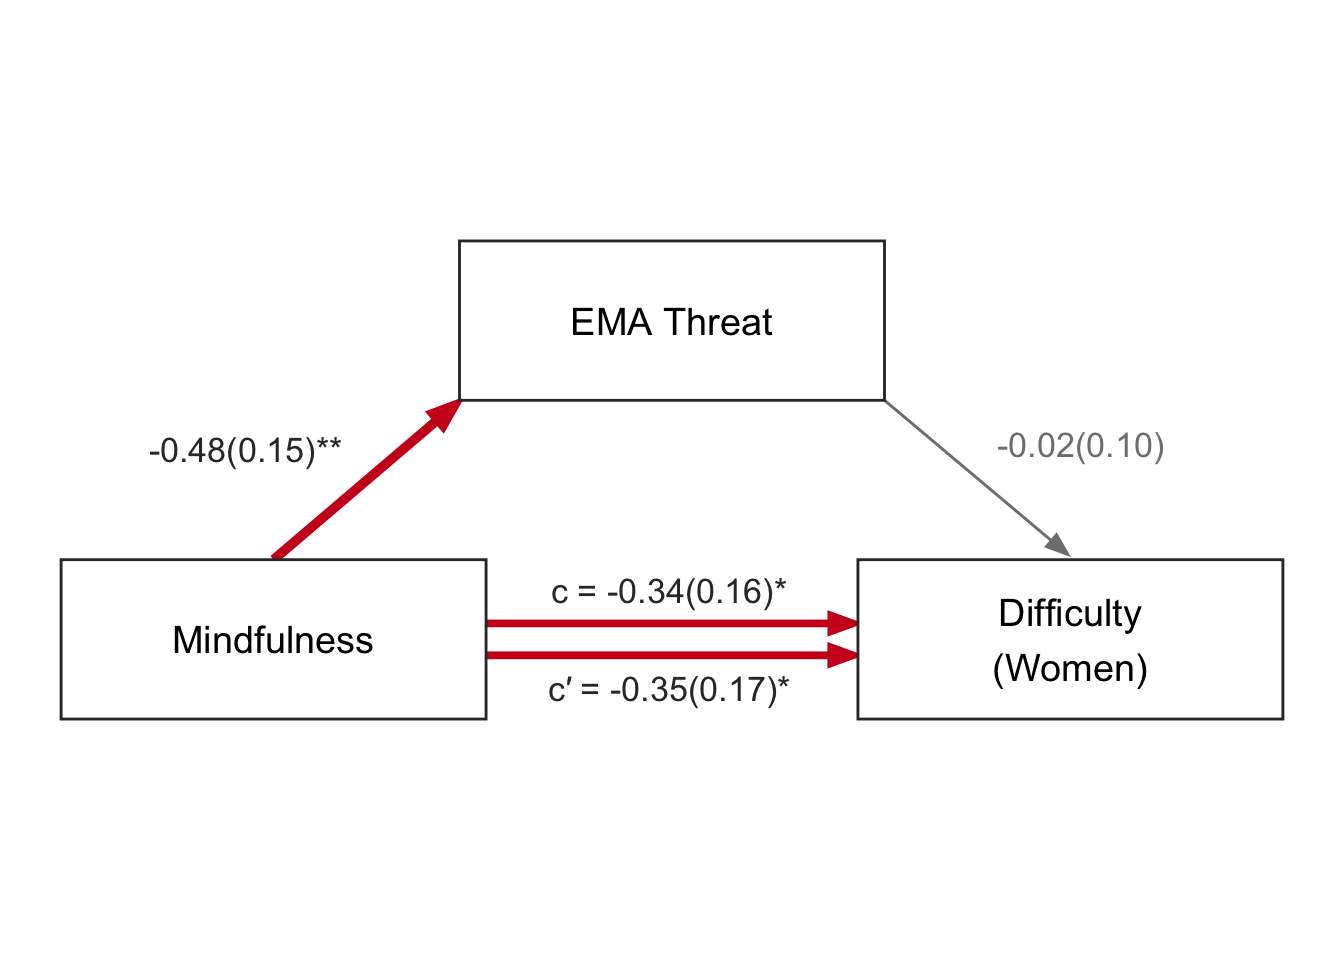
\includegraphics[keepaspectratio]{chapters/09-research-question-2_files/figure-pdf/fig-diff-wnb-1.pdf}}

}

\end{figure}%

\subsubsection{Mediation Test}\label{mediation-test-5}

See Supplementary Table~\ref{tbl-med-diff-wnb}

\begin{table}

\caption{\label{tbl-med-diff-wnb}Mediation Analysis for Difficulty at
Posttest: Women}

\centering{

\centering
\begin{tabular}[t]{lrrrr}
\toprule
Statistic & Estimate & CI Lower & CI Upper & p\\
\midrule
Avg. Causal Mediation Effect & 0.01 & -0.13 & 0.13 & 0.9034\\
Avg. Direct Effect & -0.35 & -0.70 & -0.03 & 0.0320\\
Total Effect & -0.34 & -0.66 & -0.05 & 0.0254\\
Proportion Mediated & -0.02 & -0.66 & 0.55 & 0.9068\\
\bottomrule
\multicolumn{5}{l}{\rule{0pt}{1em}\textit{Note.} Sample Size Used: 148; Simulations: 10000}\\
\end{tabular}

}

\end{table}%

\section{Unmoderated Mediation Results (preregistered
analyses)}\label{sec-preregistered}

\subsection{Confidence}\label{confidence-2}

\subsubsection{Linear Models}\label{linear-models}

\begin{table}

\caption{\label{tbl-rq2-prereg-1}Mediation Analysis for Confidence at
Posttest without Gender Moderation}

\centering{

\centering\begingroup\fontsize{8}{10}\selectfont

\resizebox{\ifdim\width>\linewidth\linewidth\else\width\fi}{!}{
\begin{tabular}[t]{>{\raggedright\arraybackslash}p{4cm}>{\raggedright\arraybackslash}p{1cm}>{\raggedright\arraybackslash}p{1cm}>{\raggedright\arraybackslash}p{1cm}>{\raggedright\arraybackslash}p{1cm}>{\raggedright\arraybackslash}p{1cm}>{\raggedright\arraybackslash}p{1cm}>{\raggedright\arraybackslash}p{1cm}>{\raggedright\arraybackslash}p{1cm}>{\raggedright\arraybackslash}p{1cm}}
\toprule
\multicolumn{1}{c}{ } & \multicolumn{3}{c}{Model 1 DV: Posttest Confidence} & \multicolumn{3}{c}{Model 2 DV: EMA Threat} & \multicolumn{3}{c}{Model 3 DV: Posttest Confidence} \\
\cmidrule(l{3pt}r{3pt}){2-4} \cmidrule(l{3pt}r{3pt}){5-7} \cmidrule(l{3pt}r{3pt}){8-10}
Predictor & Estimate & SE & p & Estimate & SE & p & Estimate & SE & p\\
\midrule
(Intercept) & -0.03 & 0.12 & 0.828 & 0.21 & 0.12 & 0.076 & 0.00 & 0.12 & 0.982\\
Condition [Mindfulness] & 0.19 & 0.11 & 0.083 & -0.35 & 0.11 & \textbf{0.002} & 0.15 & 0.11 & 0.200\\
Gender [Women or Non-binary] & -0.05 & 0.12 & 0.708 & -0.16 & 0.12 & 0.210 & -0.07 & 0.12 & 0.587\\
Baseline Score & 0.09 & 0.06 & 0.116 & 0.04 & 0.06 & 0.435 & 0.10 & 0.06 & 0.093\\
Cohort 2 & 0.10 & 0.10 & 0.351 & -0.04 & 0.10 & 0.705 & 0.09 & 0.10 & 0.375\\
\addlinespace
Cohort 3 & -0.01 & 0.15 & 0.966 & -0.11 & 0.14 & 0.464 & -0.02 & 0.14 & 0.887\\
Semester Week & 0.03 & 0.15 & 0.812 & -0.02 & 0.15 & 0.868 & 0.03 & 0.15 & 0.828\\
Posttest Test Version [B] & -0.09 & 0.11 & 0.406 & 0.11 & 0.11 & 0.329 & -0.08 & 0.11 & 0.483\\
Baseline Threat & -0.06 & 0.06 & 0.349 & 0.67 & 0.06 & \textbf{<0.001} & 0.03 & 0.09 & 0.734\\
Baseline Confidence & 0.68 & 0.07 & \textbf{<0.001} & -0.16 & 0.07 & \textbf{0.021} & 0.66 & 0.07 & \textbf{<0.001}\\
\addlinespace
EMA Threat &  &  &  &  &  &  & -0.13 & 0.08 & 0.114\\
Observations & 148 &  &  & 148 &  &  & 148 &  & \\
R2 / R2 adjusted & 0.581 / 0.554 &  &  & 0.583 / 0.556 &  &  & 0.589 / 0.559 &  & \\
\bottomrule
\end{tabular}}
\endgroup{}

}

\end{table}%

\subsubsection{Path Diagram}\label{path-diagram-6}

\begin{figure}[!hp]

\caption{\label{fig-rq2-prereg-2}Mediation Analysis for Confidence at
Posttest without Gender Moderation}

\centering{

\pandocbounded{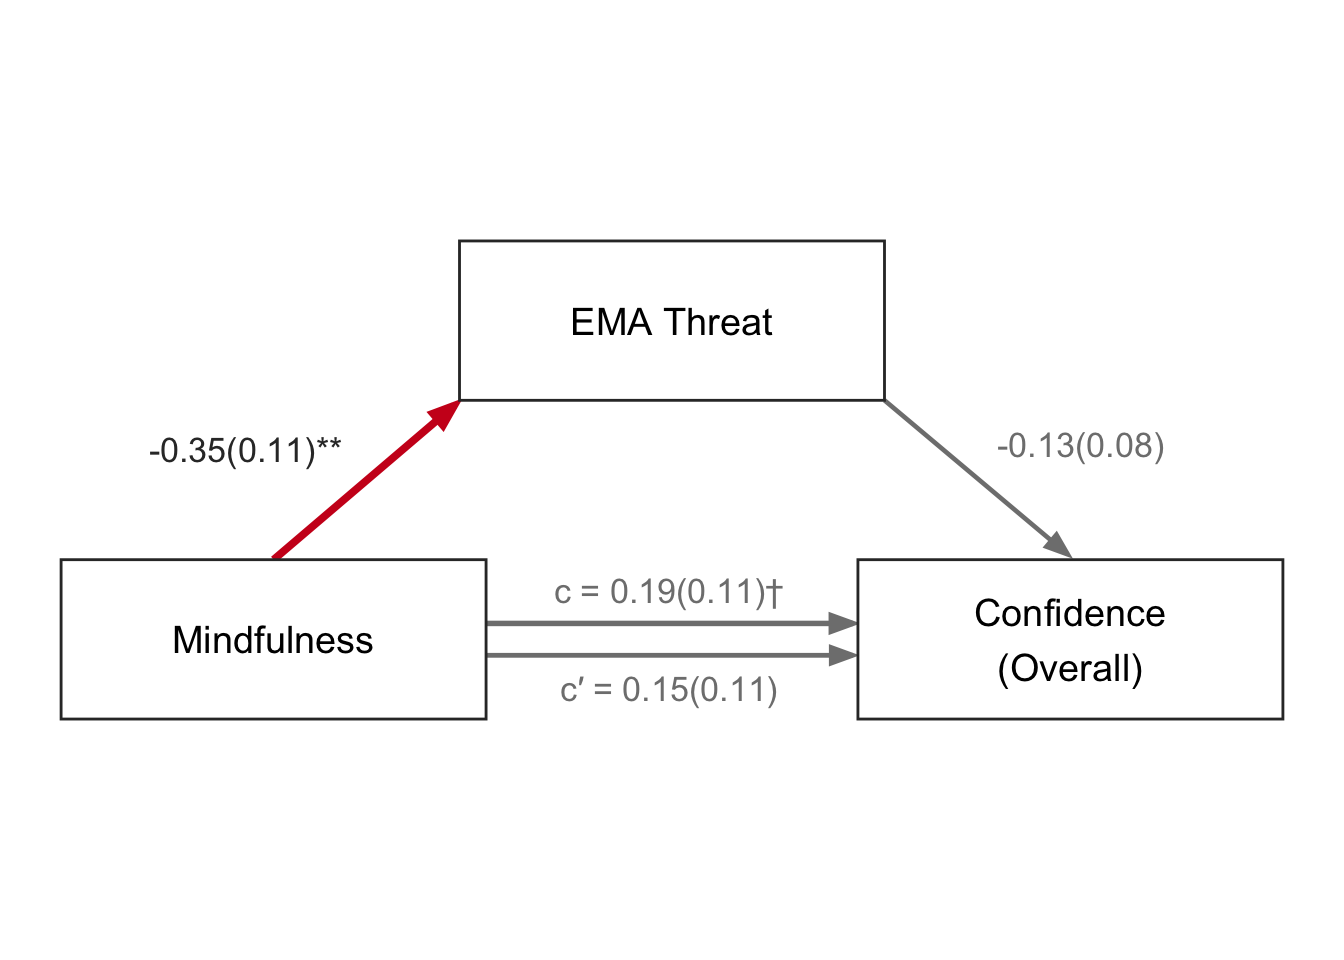
\includegraphics[keepaspectratio]{chapters/09-research-question-2_files/figure-pdf/fig-rq2-prereg-2-1.pdf}}

}

\end{figure}%

\subsubsection{Mediation Test}\label{mediation-test-6}

\begin{table}

\caption{\label{tbl-med-rq2-prereg-3}Mediation Analysis for Confidence
at Posttest without Gender Moderation}

\centering{

\centering
\begin{tabular}[t]{lrrrr}
\toprule
Statistic & Estimate & CI Lower & CI Upper & p\\
\midrule
Avg. Causal Mediation Effect & 0.05 & 0.00 & 0.13 & 0.0610\\
Avg. Direct Effect & 0.15 & -0.07 & 0.37 & 0.1890\\
Total Effect & 0.19 & -0.02 & 0.42 & 0.0816\\
Proportion Mediated & 0.24 & 0.16 & 25.32 & 0.1370\\
\bottomrule
\multicolumn{5}{l}{\rule{0pt}{1em}\textit{Note.} Sample Size Used: 148; Simulations: 10000}\\
\end{tabular}

}

\end{table}%

\subsection{Anxiety}\label{anxiety-2}

\subsubsection{Linear Models}\label{linear-models-1}

\begin{table}

\caption{\label{tbl-rq2-prereg-4}Mediation Analysis for Anxiety at
Posttest without Gender Moderation}

\centering{

\centering\begingroup\fontsize{8}{10}\selectfont

\resizebox{\ifdim\width>\linewidth\linewidth\else\width\fi}{!}{
\begin{tabular}[t]{>{\raggedright\arraybackslash}p{4cm}>{\raggedright\arraybackslash}p{1cm}>{\raggedright\arraybackslash}p{1cm}>{\raggedright\arraybackslash}p{1cm}>{\raggedright\arraybackslash}p{1cm}>{\raggedright\arraybackslash}p{1cm}>{\raggedright\arraybackslash}p{1cm}>{\raggedright\arraybackslash}p{1cm}>{\raggedright\arraybackslash}p{1cm}>{\raggedright\arraybackslash}p{1cm}}
\toprule
\multicolumn{1}{c}{ } & \multicolumn{3}{c}{Model 1 DV: Posttest Anxiety} & \multicolumn{3}{c}{Model 2 DV: EMA Threat} & \multicolumn{3}{c}{Model 3 DV: Posttest Anxiety} \\
\cmidrule(l{3pt}r{3pt}){2-4} \cmidrule(l{3pt}r{3pt}){5-7} \cmidrule(l{3pt}r{3pt}){8-10}
Predictor & Estimate & SE & p & Estimate & SE & p & Estimate & SE & p\\
\midrule
(Intercept) & 0.02 & 0.12 & 0.836 & 0.20 & 0.11 & 0.075 & -0.02 & 0.11 & 0.857\\
Condition [Mindfulness] & -0.20 & 0.11 & 0.073 & -0.32 & 0.11 & \textbf{0.004} & -0.13 & 0.11 & 0.244\\
Gender [Women or Non-binary] & 0.05 & 0.12 & 0.697 & -0.17 & 0.12 & 0.169 & 0.08 & 0.12 & 0.487\\
Baseline Score & -0.08 & 0.06 & 0.179 & 0.03 & 0.06 & 0.611 & -0.08 & 0.06 & 0.139\\
Cohort 2 & -0.03 & 0.10 & 0.738 & -0.05 & 0.10 & 0.621 & -0.02 & 0.10 & 0.816\\
\addlinespace
Cohort 3 & -0.05 & 0.15 & 0.748 & -0.13 & 0.14 & 0.376 & -0.02 & 0.14 & 0.894\\
Semester Week & -0.11 & 0.14 & 0.462 & -0.07 & 0.14 & 0.606 & -0.09 & 0.14 & 0.524\\
Posttest Test Version [B] & 0.10 & 0.11 & 0.363 & 0.10 & 0.11 & 0.365 & 0.08 & 0.11 & 0.467\\
Baseline Threat & 0.08 & 0.06 & 0.195 & 0.68 & 0.06 & \textbf{<0.001} & -0.07 & 0.08 & 0.405\\
Baseline Anxiety & 0.68 & 0.06 & \textbf{<0.001} & 0.18 & 0.06 & \textbf{0.004} & 0.65 & 0.06 & \textbf{<0.001}\\
\addlinespace
EMA Threat &  &  &  &  &  &  & 0.22 & 0.08 & \textbf{0.011}\\
Observations & 148 &  &  & 148 &  &  & 148 &  & \\
R2 / R2 adjusted & 0.581 / 0.554 &  &  & 0.592 / 0.566 &  &  & 0.601 / 0.571 &  & \\
\bottomrule
\end{tabular}}
\endgroup{}

}

\end{table}%

\subsubsection{Path Diagram}\label{path-diagram-7}

\begin{figure}[!hp]

\caption{\label{fig-rq2-prereg-5}Mediation Analysis for Anxiety at
Posttest without Gender Moderation}

\centering{

\pandocbounded{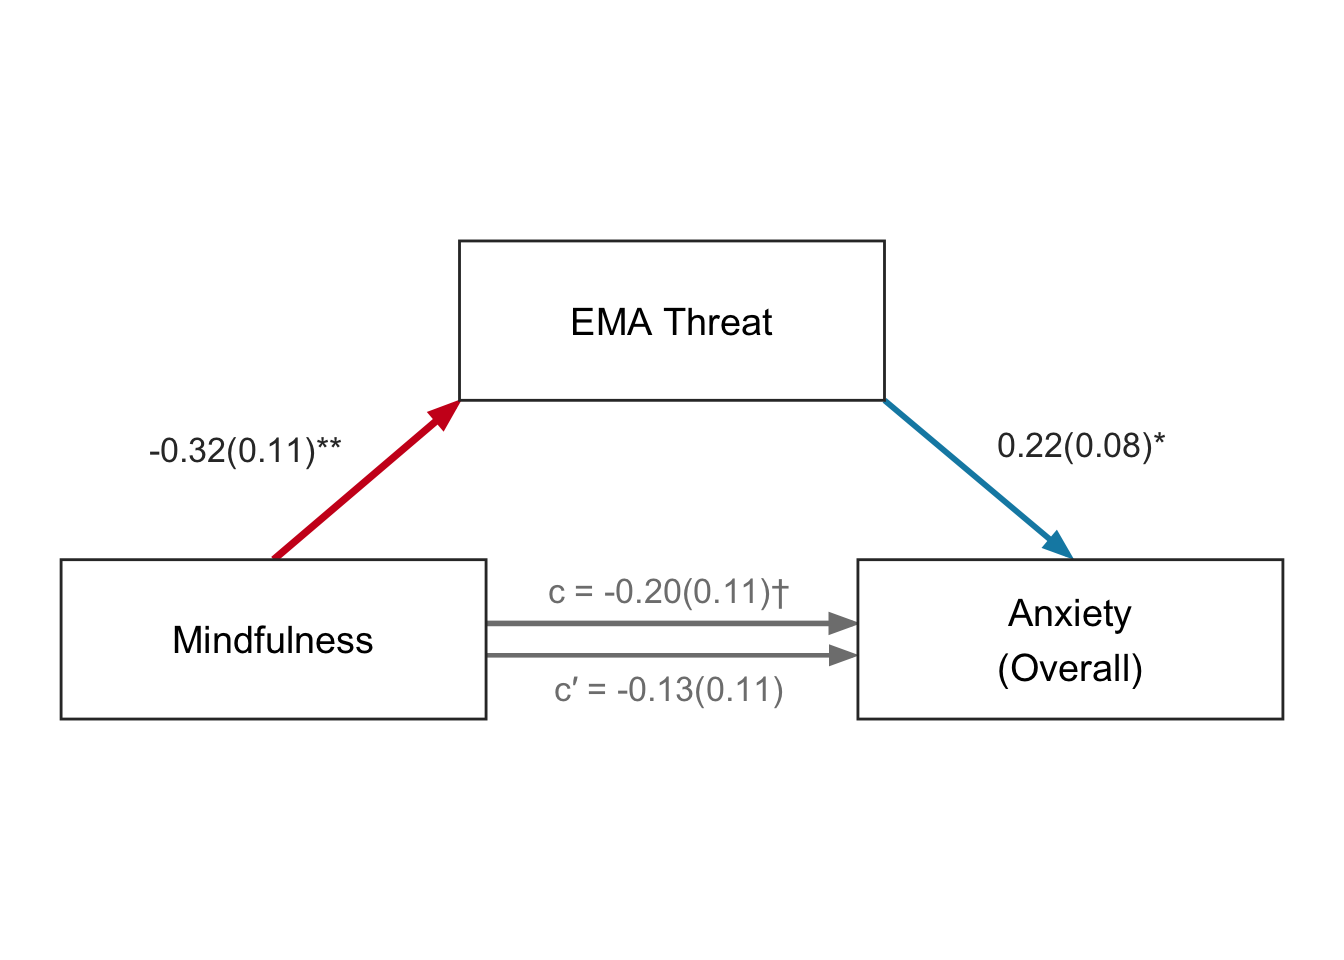
\includegraphics[keepaspectratio]{chapters/09-research-question-2_files/figure-pdf/fig-rq2-prereg-5-1.pdf}}

}

\end{figure}%

\subsubsection{Mediation Test}\label{mediation-test-7}

\begin{table}

\caption{\label{tbl-med-rq2-prereg-6}Mediation Analysis for Anxiety at
Posttest without Gender Moderation}

\centering{

\centering
\begin{tabular}[t]{lrrrr}
\toprule
Statistic & Estimate & CI Lower & CI Upper & p\\
\midrule
Avg. Causal Mediation Effect & -0.07 & -0.18 & -0.01 & 0.0202\\
Avg. Direct Effect & -0.13 & -0.36 & 0.10 & 0.2546\\
Total Effect & -0.20 & -0.42 & 0.02 & 0.0784\\
Proportion Mediated & 0.35 & -0.44 & 3.16 & 0.0930\\
\bottomrule
\multicolumn{5}{l}{\rule{0pt}{1em}\textit{Note.} Sample Size Used: 148; Simulations: 10000}\\
\end{tabular}

}

\end{table}%

\subsection{Difficulty}\label{difficulty-2}

\subsubsection{Linear Models}\label{linear-models-2}

\begin{table}

\caption{\label{tbl-rq2-prereg-7}Mediation Analysis for Difficulty at
Posttest without Gender Moderation}

\centering{

\centering\begingroup\fontsize{8}{10}\selectfont

\resizebox{\ifdim\width>\linewidth\linewidth\else\width\fi}{!}{
\begin{tabular}[t]{>{\raggedright\arraybackslash}p{4cm}>{\raggedright\arraybackslash}p{1cm}>{\raggedright\arraybackslash}p{1cm}>{\raggedright\arraybackslash}p{1cm}>{\raggedright\arraybackslash}p{1cm}>{\raggedright\arraybackslash}p{1cm}>{\raggedright\arraybackslash}p{1cm}>{\raggedright\arraybackslash}p{1cm}>{\raggedright\arraybackslash}p{1cm}>{\raggedright\arraybackslash}p{1cm}}
\toprule
\multicolumn{1}{c}{ } & \multicolumn{3}{c}{Model 1 DV: Posttest Difficulty} & \multicolumn{3}{c}{Model 2 DV: EMA Threat} & \multicolumn{3}{c}{Model 3 DV: Posttest Difficulty} \\
\cmidrule(l{3pt}r{3pt}){2-4} \cmidrule(l{3pt}r{3pt}){5-7} \cmidrule(l{3pt}r{3pt}){8-10}
Predictor & Estimate & SE & p & Estimate & SE & p & Estimate & SE & p\\
\midrule
(Intercept) & 0.06 & 0.12 & 0.647 & 0.19 & 0.11 & 0.108 & 0.06 & 0.12 & 0.629\\
Condition [Mindfulness] & -0.40 & 0.12 & \textbf{0.001} & -0.34 & 0.11 & \textbf{0.002} & -0.41 & 0.12 & \textbf{0.001}\\
Gender [Women or Non-binary] & 0.22 & 0.13 & 0.082 & -0.11 & 0.12 & 0.346 & 0.22 & 0.13 & 0.087\\
Baseline Score & -0.04 & 0.06 & 0.459 & 0.04 & 0.06 & 0.484 & -0.04 & 0.06 & 0.469\\
Cohort 2 & -0.15 & 0.11 & 0.167 & -0.04 & 0.10 & 0.733 & -0.15 & 0.11 & 0.167\\
\addlinespace
Cohort 3 & -0.18 & 0.15 & 0.246 & -0.10 & 0.15 & 0.508 & -0.18 & 0.15 & 0.243\\
Semester Week & -0.12 & 0.15 & 0.448 & -0.02 & 0.15 & 0.869 & -0.12 & 0.15 & 0.448\\
Posttest Test Version [B] & 0.05 & 0.12 & 0.699 & 0.10 & 0.11 & 0.362 & 0.05 & 0.12 & 0.688\\
Baseline Threat & -0.01 & 0.06 & 0.842 & 0.69 & 0.06 & \textbf{<0.001} & 0.00 & 0.09 & 0.991\\
Baseline Difficulty & 0.67 & 0.07 & \textbf{<0.001} & 0.15 & 0.06 & \textbf{0.020} & 0.67 & 0.07 & \textbf{<0.001}\\
\addlinespace
EMA Threat &  &  &  &  &  &  & -0.02 & 0.09 & 0.823\\
Observations & 148 &  &  & 148 &  &  & 148 &  & \\
R2 / R2 adjusted & 0.534 / 0.503 &  &  & 0.584 / 0.557 &  &  & 0.534 / 0.500 &  & \\
\bottomrule
\end{tabular}}
\endgroup{}

}

\end{table}%

\subsubsection{Path Diagram}\label{path-diagram-8}

\begin{figure}[!hp]

\caption{\label{fig-rq2-prereg-8}Mediation Analysis for Difficulty at
Posttest without Gender Moderation}

\centering{

\pandocbounded{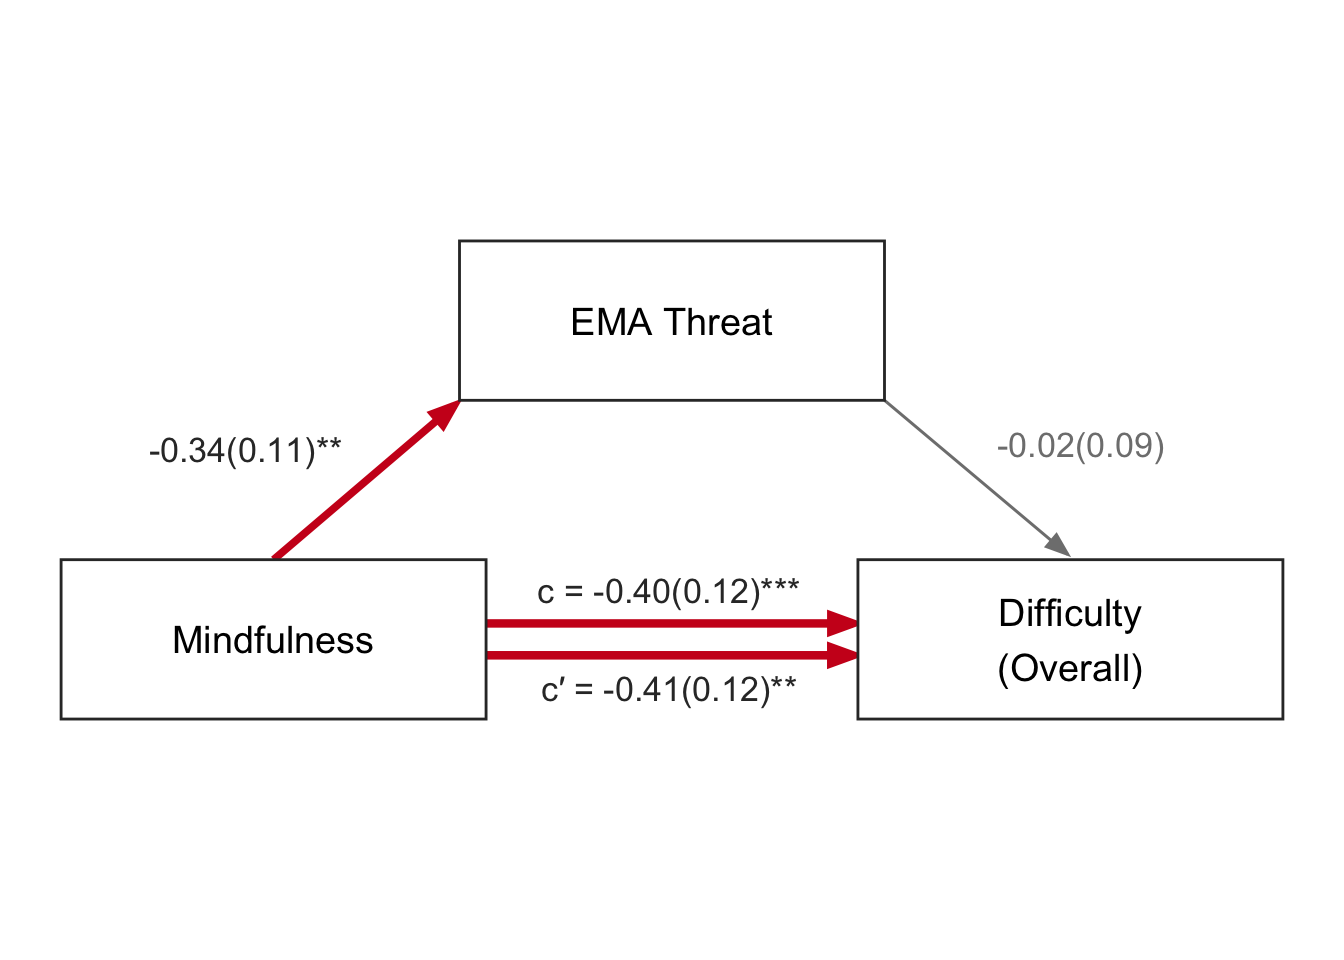
\includegraphics[keepaspectratio]{chapters/09-research-question-2_files/figure-pdf/fig-rq2-prereg-8-1.pdf}}

}

\end{figure}%

\subsubsection{Mediation Test}\label{mediation-test-8}

\begin{table}

\caption{\label{tbl-med-rq2-prereg-9}Mediation Analysis for Difficulty
at Posttest without Gender Moderation}

\centering{

\centering
\begin{tabular}[t]{lrrrr}
\toprule
Statistic & Estimate & CI Lower & CI Upper & p\\
\midrule
Avg. Causal Mediation Effect & 0.01 & -0.06 & 0.08 & 0.8550\\
Avg. Direct Effect & -0.41 & -0.65 & -0.17 & 0.0012\\
Total Effect & -0.40 & -0.63 & -0.18 & 0.0004\\
Proportion Mediated & -0.02 & -0.26 & 0.17 & 0.8550\\
\bottomrule
\multicolumn{5}{l}{\rule{0pt}{1em}\textit{Note.} Sample Size Used: 148; Simulations: 10000}\\
\end{tabular}

}

\end{table}%

\chapter{Physics Task Accuracy}\label{physics-task-accuracy}

The tables below show that there was no effect of mindfulness training
on physics task accuracy (Supplementary
Table~\ref{tbl-accuracy-results}) or learning on the PFL (Supplementary
Table~\ref{tbl-pfl-results}).

\section{Model Specification}\label{model-specification-2}

\section{Preregistered Hypotheses 1 and
4}\label{preregistered-hypotheses-1-and-4}

\begin{table}

\caption{\label{tbl-accuracy-results}Results from Mixed Effects Models
Testing Preregistered Hypotheses 1 and 4: Effects of Mindfulness
Training on Problem Solving Accuracy}

\centering{

\centering\begingroup\fontsize{8}{10}\selectfont

\resizebox{\ifdim\width>\linewidth\linewidth\else\width\fi}{!}{
\begin{tabular}[t]{>{\raggedright\arraybackslash}p{4cm}>{\raggedright\arraybackslash}p{1cm}>{\raggedright\arraybackslash}p{1cm}>{\raggedright\arraybackslash}p{1cm}>{\raggedright\arraybackslash}p{1cm}>{\raggedright\arraybackslash}p{1cm}>{\raggedright\arraybackslash}p{1cm}>{\raggedright\arraybackslash}p{1cm}>{\raggedright\arraybackslash}p{1cm}>{\raggedright\arraybackslash}p{1cm}}
\toprule
\multicolumn{1}{c}{ } & \multicolumn{3}{c}{Part1: Quantitative} & \multicolumn{3}{c}{Part2: Categorization} & \multicolumn{3}{c}{Part3: Qualitative} \\
\cmidrule(l{3pt}r{3pt}){2-4} \cmidrule(l{3pt}r{3pt}){5-7} \cmidrule(l{3pt}r{3pt}){8-10}
Predictor & Estimate & SE & p & Estimate & SE & p & Estimate & SE & p\\
\midrule
(Intercept) & 0.07 & 0.01 & \textbf{<0.001} & 0.38 & 0.02 & \textbf{<0.001} & 0.50 & 0.02 & \textbf{<0.001}\\
Cohort [Cohort 2] & 0.01 & 0.06 & 0.902 & -0.11 & 0.08 & 0.178 & -0.10 & 0.08 & 0.222\\
Cohort [Cohort 3] & 0.07 & 0.05 & 0.213 & -0.03 & 0.07 & 0.630 & -0.08 & 0.07 & 0.288\\
Semester Week & 0.01 & 0.01 & 0.339 & -0.00 & 0.01 & 0.750 & 0.01 & 0.01 & 0.675\\
Test Version [B] & 0.03 & 0.02 & 0.092 & -0.10 & 0.02 & \textbf{<0.001} & 0.21 & 0.02 & \textbf{<0.001}\\
\addlinespace
Baseline Threat & -0.04 & 0.01 & \textbf{<0.001} & -0.00 & 0.01 & 0.766 & -0.03 & 0.01 & \textbf{0.008}\\
Gender [Women or Non-binary] & 0.02 & 0.02 & 0.344 & -0.01 & 0.03 & 0.774 & -0.06 & 0.03 & \textbf{0.033}\\
Timepoint [Posttest] & 0.01 & 0.02 & 0.545 & -0.03 & 0.02 & 0.205 & 0.07 & 0.02 & \textbf{0.003}\\
Condition [Mindfulness] & 0.02 & 0.03 & 0.385 & 0.04 & 0.04 & 0.292 & -0.06 & 0.04 & 0.083\\
Timepoint [Posttest] × Condition [Mindfulness] & -0.02 & 0.04 & 0.558 & -0.05 & 0.04 & 0.277 & 0.04 & 0.05 & 0.369\\
\addlinespace
\textbf{Random Effects} & \textbf{} & \textbf{} & \textbf{} & \textbf{} & \textbf{} & \textbf{} & \textbf{} & \textbf{} & \textbf{}\\
$\sigma^2$ & 0.03 &  &  & 0.04 &  &  & 0.04 &  & \\
$\tau_{00}$ & $0.00_{Participant}$ &  &  & $0.01_{Participant}$ &  &  & $0.01_{Participant}$ &  & \\
ICC & 0.04 &  &  & 0.20 &  &  & 0.15 &  & \\
$N$ & $149_{Participant}$ &  &  & $149_{Participant}$ &  &  & $149_{Participant}$ &  & \\
\addlinespace
Observations & 295 &  &  & 298 &  &  & 298 &  & \\
Marginal $R^2$ / Conditional $R^2$ & 0.095 / 0.135 &  &  & 0.072 / 0.259 &  &  & 0.274 / 0.380 &  & \\
\bottomrule
\end{tabular}}
\endgroup{}

}

\end{table}%

\begin{tcolorbox}[enhanced jigsaw, bottomrule=.15mm, breakable, coltitle=black, rightrule=.15mm, colbacktitle=quarto-callout-note-color!10!white, leftrule=.75mm, titlerule=0mm, colframe=quarto-callout-note-color-frame, toprule=.15mm, colback=white, left=2mm, bottomtitle=1mm, opacitybacktitle=0.6, opacityback=0, toptitle=1mm, arc=.35mm, title=\textcolor{quarto-callout-note-color}{\faInfo}\hspace{0.5em}{Note}]

Supplementary Table~\ref{tbl-accuracy-results}: The estimates for the
intercept represent the overall mean score (percent correct) and
standard errors for each of the problem solving performance outcomes at
baseline. The estimate for timepoint represents the change in the
dependent variable from baseline to posttest across

\end{tcolorbox}

\section{Preregistered Hypothesis 5}\label{preregistered-hypothesis-5}

\begin{table}

\caption{\label{tbl-pfl-results}Results from Logistic Mixed Effects
Model Testing Preregistered Hypothesis 5: Effects of Mindfulness
Training on Learning During the Preparation for Future Learning Task}

\centering{

\centering\begingroup\fontsize{8}{10}\selectfont

\resizebox{\ifdim\width>\linewidth\linewidth\else\width\fi}{!}{
\begin{tabular}[t]{>{\raggedright\arraybackslash}p{4cm}>{\raggedright\arraybackslash}p{1cm}>{\raggedright\arraybackslash}p{1cm}>{\raggedright\arraybackslash}p{1cm}>{}p{1cm}>{}p{1cm}>{}p{1cm}>{}p{1cm}>{}p{1cm}>{}p{1cm}}
\toprule
\multicolumn{1}{c}{ } & \multicolumn{3}{c}{PFL Correctness} \\
\cmidrule(l{3pt}r{3pt}){2-4}
Predictor & Odds Ratios & SE & p\\
\midrule
(Intercept) & 0.23 & 0.06 & \textbf{<0.001}\\
Cohort [Cohort 2] & 1.13 & 1.04 & 0.894\\
Cohort [Cohort 3] & 0.51 & 0.41 & 0.403\\
Semester Week & 1.10 & 0.16 & 0.521\\
Baseline Threat & 0.86 & 0.11 & 0.234\\
\addlinespace
Gender [Women or Non-binary] & 0.37 & 0.13 & \textbf{0.005}\\
Question [2] & 4.87 & 1.59 & \textbf{<0.001}\\
Condition [Mindfulness] & 1.42 & 0.64 & 0.433\\
Question [2] × Condition [Mindfulness] & 0.91 & 0.52 & 0.873\\
\textbf{Random Effects} & \textbf{} & \textbf{} & \textbf{}\\
\addlinespace
$\sigma^2$ & 3.29 &  & \\
$\tau_{00}$Participant & 0.62 &  & \\
ICC & 0.16 &  & \\
$N$Participant & 149 &  & \\
Observations & 298 &  & \\
\addlinespace
Marginal $R^2$ / Conditional $R^2$ & 0.235 / 0.356 &  & \\
\bottomrule
\end{tabular}}
\endgroup{}

}

\end{table}%

\begin{tcolorbox}[enhanced jigsaw, bottomrule=.15mm, breakable, coltitle=black, rightrule=.15mm, colbacktitle=quarto-callout-note-color!10!white, leftrule=.75mm, titlerule=0mm, colframe=quarto-callout-note-color-frame, toprule=.15mm, colback=white, left=2mm, bottomtitle=1mm, opacitybacktitle=0.6, opacityback=0, toptitle=1mm, arc=.35mm, title=\textcolor{quarto-callout-note-color}{\faInfo}\hspace{0.5em}{Note}]

Supplementary Table~\ref{tbl-pfl-results}: The odds ratio for the
intercept term represents the odds of getting question 1 correct
compared to incorrect. The odds ratio for the question × condition
interaction term represents the difference in odds of getting question 2
correct between conditions, above and beyond any condition differences
on question 1 and overall differences on question 2, compared to
question 1. P-values below .05 are indicated by bold font.

\end{tcolorbox}

\bookmarksetup{startatroot}

\chapter*{References}\label{references}
\addcontentsline{toc}{chapter}{References}

\markboth{References}{References}

\phantomsection\label{refs}
\begin{CSLReferences}{1}{0}
\bibitem[\citeproctext]{ref-belenky2012}
Belenky, Daniel M, and Timothy J Nokes-Malach. 2012. {``Motivation and
Transfer: The Role of Mastery-Approach Goals in Preparation for Future
Learning.''} \emph{The Journal of the Learning Sciences} 21 (3):
399--432. \url{https://doi.org/10.1080/10508406.2011.651232}.

\bibitem[\citeproctext]{ref-hardiman1989}
Hardiman, Pamela Thibodeau, Robert Dufresne, and Jose P Mestre. 1989.
{``The Relation Between Problem Categorization and Problem Solving Among
Experts and Novices.''} \emph{Memory \& Cognition} 17 (5): 627--38.

\bibitem[\citeproctext]{ref-schwartz2004inventing}
Schwartz, Daniel L, and Taylor Martin. 2004. {``Inventing to Prepare for
Future Learning: The Hidden Efficiency of Encouraging Original Student
Production in Statistics Instruction.''} \emph{Cognition and
Instruction} 22 (2): 129--84.

\bibitem[\citeproctext]{ref-weinlader2019}
Weinlader, Nolan K., Eric Kuo, Benjamin M. Rottman, and Timothy J.
Nokes-Malach. 2019. {``A New Approach for Uncovering Student Resources
with Multiple-Choice Questions.''} In, 621--26. American Association of
Physics Teachers. \url{https://doi.org/10.1119/perc.2019.pr.Weinlader}.

\end{CSLReferences}




\end{document}
